\documentclass{article}
\usepackage{iclr2025_conference,times}


\usepackage[utf8]{inputenc} % allow utf-8 input
\usepackage[T1]{fontenc}    % use 8-bit T1 fonts
% \usepackage{hyperref}       % hyperlinks
\usepackage{url}            % simple URL typesetting
\usepackage{booktabs}       % professional-quality tables
\usepackage{amsfonts}       % blackboard math symbols
\usepackage{amssymb}
\usepackage{nicefrac}       % compact symbols for 1/2, etc.
\usepackage{microtype}      % microtypography
\usepackage{xcolor}         % colors

% \hypersetup{
% colorlinks=blue,
% linkcolor=blue,
% citecolor=blue,
% breaklinks=true
% urlcolor=cyan,
% pdftitle={Overleaf Example},
% pdfpagemode=FullScreen,
% }

\usepackage[hidelinks,colorlinks=true,citecolor=blue,linkcolor=blue]{hyperref}
% \usepackage{natbib}
% \usepackage{color}
% \usepackage{amsfonts}      
% \usepackage{url}
% \usepackage{amsmath}
% \usepackage{amsthm}
% \usepackage{wrapfig}
\usepackage{mathtools}
\usepackage{amsthm}
\usepackage{tikz}
% \usepackage{subfig}
\usepackage{algorithmic}
\usepackage{footmisc}
\usepackage{bibentry}
\nobibliography*
\DeclarePairedDelimiter{\ceil}{\lceil}{\rceil}
\usepackage{physics}
\usepackage{mathrsfs}
\mathtoolsset{showonlyrefs}
\usepackage{etoolbox}
\usepackage{makecell}
\usepackage[ruled]{algorithm2e}
\DontPrintSemicolon
\usepackage{enumerate}
\usepackage{lastpage}
\usepackage{float}
\usepackage{verbatim}
\usepackage{graphicx}
\usepackage{subcaption}
\usepackage{setspace}
\usepackage{enumitem}
% \usepackage{cite} 
\usepackage{thmtools, thm-restate}
% \declaretheorem{theorem}
% \newtheorem*{assumption*}{Assumption}

\newcommand{\explain}[1]{\tag*{(#1)}}
\newcommand{\explaind}[2]{\makebox[0.85\textwidth]{$\displaystyle#1$\hfill(#2)}}
% \newcommand{\explaind}[2]{\hspace{#1\textwidth}  \text{(#2)}}
% \newcommand{\explain}[1]{&& \mbox{(#1)}}
% \newcommand{\test}[1]{\ifmeasuring@\text{#1}\else\omit\hfill$\displaystyle#1$\fi\ignorespaces}
\newcommand{\explainnl}[1]{\intertext{\hfill (#1)}}


\newcommand{\normlp}[1]{\norm{{#1}}_{\E,p}}
\newcommand{\normlpn}[1]{\norm{\norm{#1}}_{\E,p}}
\newcommand{\blue}[1]{{\color{blue} {#1}}}
\newcommand{\lsz}[1]{({\color{magenta} {Shuze: #1}})}
\newcommand{\jw}[1]{({\color{magenta} {Jiuqi: #1}})}
\newcommand{\ehb}[1]{({\color{violet} {Ethan: #1}})}
\newcommand{\sz}[1]{({\color{red} {Shangtong: #1}})}
% \newcommand{\newtext}[1]{{\color{teal}#1}}
\newcommand{\newtext}[1]{{#1}}

\newcommand{\fS}{\mathcal{S}}
\newcommand{\fA}{\mathcal{A}}
\newcommand{\fY}{\mathcal{Y}}
\newcommand{\fB}{\mathcal{B}}
\newcommand{\fZ}{\mathcal{Z}}
\newcommand{\fW}{\mathcal{W}}
\newcommand{\fF}{\mathcal{F}}
\newcommand{\fO}{\mathcal{O}}
\newcommand{\fH}{\mathcal{H}}
\newcommand{\fN}{\mathcal{N}}
\newcommand{\fX}{\mathcal{X}}
\newcommand{\fL}{\mathcal{L}}
\newcommand{\vw}{w}
\newcommand{\R}{\mathbb{R}}
\newcommand{\N}{\mathbb{N}}
\newcommand{\E}{\mathbb{E}}
\newcommand{\V}{\mathbb{V}}
\newcommand{\one}{\mathbf{1}}
\newcommand{\nsa}{{|\fS \times \fA|}}
\newcommand{\ns}{{|\fS|}}
\newcommand{\na}{{|\fA|}}
\newcommand{\ny}{{|\fY|}}
\newcommand{\bop}{\mathcal{T}}
\newcommand{\pdisg}{G^{\text{PDIS}}}
\newcommand{\isg}{G^{\text{IS}}}
\newcommand{\ig}{{\text{IG}}}
\newcommand{\nexp}[1]{\exp\left(-\frac{1}{2}\left({#1}\right)\right)}
\newcommand{\tb}[1]{{\textbf{#1}}}
\newcommand{\pbop}[2]{\omega_{f_{n, #1, #2}}\bop_{#2}}
\newcommand{\indot}[2]{{\left<#1, #2\right>}}
\newcommand{\cred}[1]{{\color{red}#1}}
\newcommand*\diff{\mathop{}\!\mathrm{d}}
% \DeclarePairedDelimiter\floor{\lfloor}{\rfloor}
\def\argmin{\qopname\relax n{argmin}}
\newcommand{\dsf}{\delimitershortfall=-1pt }
\newcommand{\attn}{\text{LinAttn}}
\newcommand{\nattn}{\text{Attn}}
\newcommand{\twohead}{\text{TwoHead}}
\newcommand{\tf}{\text{TF}}
\newcommand{\ntf}{\widetilde{\tf}}
\newcommand{\softmax}[1]{\text{softmax}\qty(#1)}
\newcommand{\paren}[1]{{\left(#1\right)}}
\renewcommand{\contentsname}{Table of Contents}
\newcommand{\td}{\text{TD}}
\newcommand{\mdp}{\text{MDP}}
\newcommand{\bartd}{\overline{\text{TD}}}
\newcommand{\rg}{\text{RG}}
\newcommand{\tdlambda}{\text{TD($\lambda$)}}
\newcommand{\uniform}[1]{{\text{Uniform}\left[#1\right]}}
\newcommand{\diag}{\text{diag}}

\newtheorem{theorem}{Theorem}
\newtheorem{xtheorem}{Theorem}[section]
\newtheorem{proposition}{Proposition}%[section]
\newtheorem{lemma}{Lemma}[subsection]%[Lemma]
\newtheorem{corollary}{Corollary}
\newtheorem{assumption}{Assumption}[section]
\newtheorem{xassumption}{Assumption}[section]
\newtheorem{definition}{Definition}
\newtheorem{remark}{Remark}

\newtheorem{manualassumptioninner}{Assumption}
\newenvironment{manualassumption}[1]{%
  \renewcommand\themanualassumptioninner{#1}%
  \manualassumptioninner
}{\endmanualassumptioninner}
%\renewcommand{\baselinestretch}{0.97}

\allowdisplaybreaks





\title{Transformers Can Learn \\ Temporal Difference Methods for \\ In-Context  Reinforcement Learning}
% The \author macro works with any number of authors. There are two commands
% used to separate the names and addresses of multiple authors: \And and \AND.
%
% Using \And between authors leaves it to LaTeX to determine where to break the
% lines. Using \AND forces a line break at that point. So, if LaTeX puts 3 of 4
% authors names on the first line, and the last on the second line, try using
% \AND instead of \And before the third author name.


% \author{
    % Jiuqi Wang , Ethan Blaser$^*$, Hadi Daneshmand, Shangtong Zhang
% }

\author{Jiuqi Wang\thanks{Equal contribution. The order is determined by tossing a fair coin.} \\
University of Virginia\\
\texttt{jiuqi@email.virginia.edu} \\
\And
Ethan Blaser\footnotemark[1] \\
University of Virginia \\
\texttt{blaser@email.virginia.edu} \\
\AND
Hadi Daneshmand\footnotemark[2]\thanks{Work performed while affiliated with MIT LIDS/Boston University.} \\
 University of Virginia\\
\texttt{dhadi@virginia.edu} \\
\And
Shangtong Zhang \\
University of Virginia \\
\texttt{shangtong@virginia.edu}}

\iclrfinalcopy
\begin{document}

\maketitle


\begin{abstract}

Traditionally, reinforcement learning (RL) agents learn to solve new tasks by updating their neural network parameters through interactions with the task environment. However, recent works demonstrate that some RL agents, after certain pretraining procedures, can learn to solve unseen new tasks without parameter updates, a phenomenon known as in-context reinforcement learning (ICRL). The empirical success of ICRL is widely attributed to the hypothesis that the forward pass of the pretrained agent neural network implements an RL algorithm. 
In this paper,
we support this hypothesis by showing, both empirically and theoretically,
that when a transformer is trained for policy evaluation tasks,
it can discover and learn to implement temporal difference learning in its forward pass. %by itself.
% However, no prior works have demonstrated a precise equivalence between a forward pass and any specific RL algorithm, even in simplified settings like transformers with linear attention. 
% In this paper, we support this hypothesis by presenting the first proof by construction demonstrating that transformers with linear attention can implement temporal difference (TD) learning in the forward pass --- referred to as in-context TD. We also provide theoretical analysis and empirical evidence demonstrating the emergence of in-context TD after training the transformer with a multi-task TD algorithm, offering the first constructive explanation for transformers' ability to perform in-context reinforcement learning.
    
    % Furthermore, we also prove that transformers are expressive enough to implement many other policy evaluation algorithms in the forward pass, including residual gradient, TD with eligibility trace, and average-reward TD.

    

% In-context learning refers to the learning ability of a model during inference time without adapting its parameters. The input (i.e., prompt) to the model (e.g., transformers) consists of both a context (i.e., instance-label pairs) and a query instance. The model is then able to output a label for the query instance according to the context during inference. A possible explanation for in-context learning is that the forward pass of (linear) transformers implements iterations of gradient descent on the instance-label pairs in the context. In this paper, 
\end{abstract}

\section{Introduction}
In reinforcement learning (RL, \citet{sutton2018reinforcement}), an agent typically learns to solve new tasks by updating its neural network parameters based on interactions with the task environment.
For example,
the DQN agent \citep{mnih2015human} incrementally updates the parameters of its $Q$-network while playing the Atari games \citep{bellemare13arcade}.
However,
recent works (e.g., \citet{duan2016rl,wang2016learning,laskin2022context}) 
demonstrate that RL can also occur without any parameter updates.
% Specifically,
% after certain pretraining procedures (on some task distribution),
% some RL agents
% typically based on transformers \citep{vaswani2017},
% can learn to solve new out-of-distribution tasks without updating their network parameters.
These works demonstrate that an RL agent with \emph{fixed pretrained parameters} can take as input its observation history in the new task (referred to as context) and output good actions for that task. 
Specifically, let $\tau_t \doteq (S_0, A_0, R_1, \dots, S_{t-1}, A_{t-1}, R_t)$ be a sequence of state-action-reward triples that an agent obtains until time $t$ in some new task.
This $\tau_t$ is referred to as the \emph{context}. The agent then outputs an action $A_t$ based on the context $\tau_t$ and the current state $S_t$ without updating its parameters.
Notably, the context can span multiple episodes.
As the context length increases, action quality improves, suggesting that this improvement is not due to memorized policies encoded in the fixed parameters. Instead, it indicates that a reinforcement learning process occurs during the forward pass as the agent processes the context, a phenomenon termed in-context reinforcement learning (ICRL), where RL occurs at inference time within the forward pass.
See \citet{moeini2025survey} for a comprehensive survey of ICRL.

Previous works (e.g., \citet{lin2023transformers}) understand the ICRL phenomenon from the supervised pretraining perspective,
where during the pretraining stage,
the RL agent is explicitly tasked to imitate the behavior of some existing RL algorithms.
It is therefore not surprising that the pretrained agent neural network implements the corresponding RL algorithm in its forward pass.
This paper
instead provides the first theoretical analysis of the emergence of ICRL from reinforcement pretraining,
where in the pretraining stage,
the RL agent is only asked to complete some task, but there is no constraint on how it should complete it.
ICRL emerges in the sense that the agent neural network itself discovers and implements a certain RL algorithm in the forward pass.

% Previous works \citep{lin2023transformers} support this claim by demonstrating behavioral similarities (i.e., input-output matching) between the pretrained fixed-weight transformers and known RL algorithms (e.g. UCB-VI~\citep{azar2017minimax}). 
% However, \textbf{there has been no proof identifying an exact equivalence between any known RL algorithm and the forward pass of a neural network, even in simplified cases such as transformers with linear attention}.
% This work provides the first such proof.

%Most existing works in ICRL are concerned with ICRL for control. Let $\tau_t \doteq (S_0, A_0, R_1, \dots, S_{t-1}, A_{t-1}, R_t)$ be a sequence of state-action-reward triples that an agent obtains by executing some fixed policy $\pi$ until time $t$ in some new task, i.e., this $\tau_t$ is the \emph{context}. ICRL for control expects the agent to output a good action $A_{t}$ taking the context $\tau_t$ and the current state $S_{t}$ as inputs, without parameter updates.
% \citep{laskin2022context,raparthy2023generalization,sinii2023context,zisman2023emergence,krishnamurthy2024can,lee2024supervised,park2024llm,brooks2024large}.
Although most existing ICRL studies focus on control tasks (i.e., outputting actions given a state and context), 
to better understand ICRL,
in this work, we investigate ICRL for policy evaluation, as it is widely known in the RL community that understanding policy evaluation is often the first step toward understanding control \citep{sutton2018reinforcement}. 
Specifically, 
suppose an agent with fixed pretrained parameters follows some fixed policy $\pi$ in a new task.
We explore how the agent can estimate the value function $v_\pi(s)$ for a given state $s$ based on its context $\tau_t$\footnote{We, of course, also need to provide the discount factor to the agent. We ignore it for now to simplify the presentations.} without parameter updates.
We call this \emph{in-context policy evaluation}
and believe that understanding it will pave the way for a comprehensive understanding of ICRL.
We demonstrate that ICRL can emerge even with simplified neural network architectures, 
e.g.,
transformer \citep{vaswani2017} with linear attention\footnote{Linear attention is a widely used transformer variant for simplifying both computation and analysis \citep{katharopoulos2020transformers,wang2020linformer,schlag2021linear,choromanski2020rethinking, mahankali2023one,ahn2023linear, vonoswald2023transformers, von2023uncovering, wu2023many, ahn2024transformers, gatmiry2024can, zhang2024trained,zheng2024mesa, sander2024transformers}.}.

\begin{figure}[h]
\begin{minipage}{0.4\textwidth}
    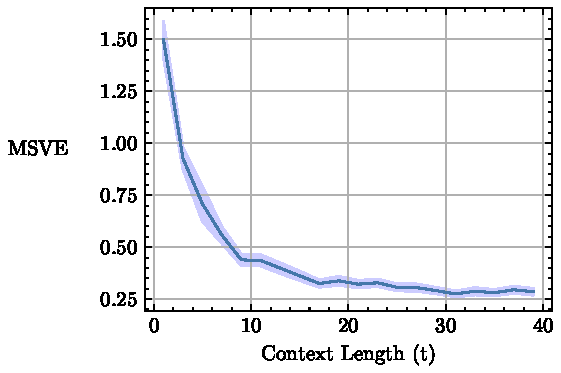
\includegraphics[width=\textwidth]{img/msve_vs_context_length.pdf}
\end{minipage}
\begin{minipage}{0.6\textwidth}
    \begin{align}
        \underbrace{S_0, A_0, R_1, \dots, S_{t-1}, A_{t-1}, R_t, s}_{\text{input: context $\tau_t$ + query $s$}} \overset{\text{$\tf_{\theta_*}$}}{ \xrightarrow{\hspace*{0.5cm}} } \underbrace{v(s)}_{\text{output}}\approx v_\pi(s)
    \end{align}
\end{minipage}
    \captionof{figure}{\label{fig: icrl demo} A transformer capable of in-context policy evaluation.
    This 15-layer transformer $\tf_{\theta_*}$ takes the context $\tau_t$ and a state of interest $s$ as input and outputs $\tf_{\theta_*}(\tau_t, s)$ as the estimation of the state value $v_\pi(s)$.
    The $y$-axis is the mean square value error (MSVE) $ \sum_s d_\pi(s) \qty(\tf_{\theta_*}(\tau_t, s)- v_\pi(s))^2$, with $d_\pi(s)$ being the stationary state distribution.
    The curves are averaged over 300 randomly generated policy evaluation tasks, with shaded regions being standard errors.
    The tasks vary in state space, transition function, reward function, and policy.
    Yet a single $\theta_*$ is used for all tasks.
    See Appendix~\ref{appendix: demo} for more details.
    }
\end{figure}
% \begin{figure}[h]
%     \centering
%     \includegraphics[width=0.5\linewidth]{img/avg_msve_vs_context_length.pdf}
%     \caption{A transformer that is capable of in-context policy evaluation.
%     This 6-layer transformer $\tf_{\theta_*}$ takes the context $\tau_t$ and a state of interest $s$ as input and output $\tf_{\theta_*}(\tau_t, s)$ as the estimation of the value funciton $v_\pi(s)$.
%     The $y$-axis is the expected value estimation error $\text{MSVE}(s) \doteq \sum_s d_\pi(s) \qty(\tf_{\theta_*}(\tau_t, s)- v_\pi(s))^2$ with $d_\pi(s)$ being the stationary state distribution.
%     The curves are averaged over 250 randomly generated policy evaluation tasks with shaded regions being standard errors.
%     Those tasks vary in state space, transition function, reward function, and policy.
%     Yet a single $\theta_*$ is used for all those tasks.
%     See \ref{} for more details. 
%     }
%     \label{fig: icrl demo}
% \end{figure}

Figure~\ref{fig: icrl demo} provides a concrete example of a transformer capable of in-context policy evaluation.
To our knowledge, this is the first empirical demonstration of in-context policy evaluation. 
Let $\tf_{\theta_*}$ denote the transformer used in Figure~\ref{fig: icrl demo} with parameters $\theta_*$.
% Then there exists some transformer parameter $\theta_*$ such that $\tf_{\theta_*}(\tau_t, s)$ approximates the value function $v_\pi(s)$ well for any $s$ \ehb{Is there necessarily this $\theta_*$?} \sz{We only claim existence, not uniqueness.} \ehb{but even with claiming existence, doesn't that require that the value function is realizable?}.
Figure~\ref{fig: icrl demo} demonstrates that the value approximation error of this transformer drops when the context length $t$ increases even though $\theta_*$ remains fixed. 
Notably, this improvement cannot be attributed to $\theta_*$ hard-coding the true value function. 
The approximation error in Figure~\ref{fig: icrl demo} is averaged over a wide range of tasks and policies, each with distinct value functions, while only a single $\theta_*$ is used. 
% We observe that $\tf_{\theta_*}(\tau_t, s)$ can approximate $v_\pi(s)$ well for any tested task and any policy,
% with a single fixed $\theta_*$.
The only plausible explanation seems to be that the transformer $\tf_{\theta_*}$ is able to perform some policy evaluation algorithm in the forward pass to process the context and thus predict the value of $s$.
% \ehb{I moved this paragraph to here. Not sure if you agree with its placement}. 
This immediately raises two key questions:
\begin{enumerate}[topsep=0pt,itemsep=-1ex,partopsep=1ex,parsep=1ex, start=1, label={ (Q\arabic*)}]
    \item What is the specific policy evaluation algorithm that $\tf_{\theta_*}$ is implementing? \label{Q1}
    \item What kind of pretraining can generate such a powerful transformer? \label{Q2}
\end{enumerate}
This work aims to answer these questions to better understand in-context RL for policy evaluation.
To this end, this work makes three contributions.

First, we confirm the existence of such a $\theta_*$ by construction.
We prove that this $\theta_*$ enables in-context policy evaluation because the layer-by-layer forward pass of $\tf_{\theta_*}$ is precisely equivalent to the iteration-by-iteration updates of a batch version of temporal difference learning (TD, \citet{sutton1988learning}). 
To summarize, a short answer to \ref{Q1} is ``TD.''
\tb{This is the first time that a pretrained agent neural network for ICRL is fully white-boxed}.
Furthermore,
we also prove by construction that transformers are capable of implementing many other policy evaluation algorithms, including TD($\lambda$) \citep{sutton1988learning}, residual gradient \citep{baird1995residual}, and average reward TD \citep{tsitsiklis1999average}.

Second, we empirically demonstrate that this $\theta_*$ naturally emerges after we regard $\tf_\theta$ as a standard nonlinear function approximator and train it using nonlinear TD on multiple randomly generated policy evaluation tasks (similar to training a single DQN agent on multiple Atari games).
This empirical finding is surprising because the pretraining only drives $\tf_\theta$ to output good value estimates.
%(cf. DQN's $Q$-network is trained to output approximations of the optimal action value function). 
There is no explicit mechanism that forces the transformer's weights to
implement TD in its forward pass (cf. that the forward pass of DQN's $Q$-network can be anything as long as it outputs good action value approximations). 
Despite having the capacity to implement other algorithms like residual gradient, the pretraining process consistently leads the transformer weights to converge to those that implement TD.
This observation parallels the historical development of the RL community itself, where TD became the favored method for policy evaluation after extensive trial-and-error with alternative approaches.
%\ehb{There is not any process that forces the transformer weights to converge to $\theta_*$ which implement TD in its forward pass. Despite having the capacity to implement other algorithms like residual gradient, the pretraining process lea to the transformer weights to converge to those that implement TD, which mirrors the historical development of the RL community—where TD became the preferred method for policy evaluation after extensive trial-and-error with alternatives.}
%But there is not any process that forces the forward pass to be equivalent to TD (cf. the forward pass of DQN's $Q$-network can be anything as long as it outputs good action value approximation). 
%The pretraining procedure itself decides that implementing TD in the forward pass is a reasonably good solution compared with others, 
%e.g., it does not end up with implementing the residual gradient despite that it has the capability to do so.
%This is very similar to the development of the RL community in the past forty years.
%No one forces the community to do policy evaluation with TD but the community seems to gradually converge to an agreement that TD is a good solution for policy evaluation,
%after numerous manual trial-and-errors of many other possible policy evaluation methods (e.g., residual gradient).
Thus, a short answer to Question \ref{Q2} is also ``TD.''
Naturally, this leads to our third and final question.
\begin{enumerate}[topsep=0pt,itemsep=-1ex,partopsep=1ex,parsep=1ex, start=3, label={ (Q\arabic*)}]
    \item Why does TD pretraining give rise to in-context TD? \label{Q3}
\end{enumerate}
Our third contribution addresses this question by proving that the parameters $\theta_*$ that implement TD in the forward pass lie in an invariant set of the TD pretraining algorithm.
% \textcolor{red}{hadi: I think that we should say our analysis is for a single layer network similar to \cite{zhang2023trained} and \cite{wu2023many}}
It is, of course, not a complete answer. 
Similar to \citet{wu2023many,zhang2024trained}, we only prove the single-layer case, and we do not prove that the parameters will surely converge to this invariant set.
However, we argue that our invariant set analysis and the techniques developed to prove it are a significant step toward future work that can fully characterize how in-context reinforcement learning emerges from reinforcement pretraining.



\section{Related Works}

Our first question \ref{Q1} is closely related to the expressivity of neural networks \citep{siegelmann1992computational,graves2014neural,jastrzkebski2017residual,hochreiter2001meta, lu2017expressive}.
Per the universal approximation theorem~\citep{hornik1989universal, cybenko1989approximation,leshno1993multilayer,bengio2017deep},
sufficiently wide neural networks can approximate any function arbitrarily well.
However, this theorem focuses only on input-output behavior, meaning that given the same input, the network will produce similar outputs as the target function.
It does not say anything about how the forward pass is able to produce the desired outputs, nor how the number of layers affects the approximation error.
% \textcolor{red}{hadi:I think that main problem with universal approximation is that the parameters may change with the task and data. The parameters are not fixed for different tasks. It can not explain fig1 as it may need to change the parameter for more inputs.}. 
% \sz{Can we use UA to argue that it can actually approximate an algorithm? If the network approximates an algoirthm well (using UA), then it doesn't need to change parameters when data and task change.} \textcolor{purple}{hadi: Then the approximation error grows with the number of layers. But, maybe we can use the universal approximator to prove that they can implement algorithms. I do not know. } \ehb{My undestanding is that the RL algorithm is just some kind of special/complicated map between the context space to some number corresponding to the value function. So it is a "function" (otherwise we wouldn't be able to demonstrate transformers can implement this algorithm in context.) }
In the supervised learning community, there are a few works that are able to white-box the forward pass of neural networks to some extent \citep{frosst2017distilling, alvarez2018towards,chan2022redunet,yu2023white,vonoswald2023transformers,ahn2024transformers}. 
But in the RL community, this work is, to our knowledge, the first to white-box how the forward pass of a pretrained transformer can implement RL algorithms.
Notably, \citet{lin2023transformers} also construct some weights of transformer such that the forward pass of the transformer can implement some RL algorithm.
However,
their constructed transformer is overly complicated and there is no evidence that their weight construction can emerge through any kind of pretraining in practice.
% Although this study primarily focuses on ICRL for policy evaluation and leaves the exploration of ICRL for control to future work, it represents the first step toward understanding how pretrained neural networks can implement RL algorithms in context.
% Notably,
% \citet{lin2023transformers} also also investigate how different RL algorithms

Our second question \ref{Q2} is closely related to the pretraining in ICRL,
which can be divided into supervised pretraining and reinforcement pretraining.
In supervised pretraining,
the agent is explicitly tasked with imitating the behavior of some existing RL algorithms demonstrated in an offline dataset \citep{xu2022prompting,laskin2022context,raparthy2023generalization,sinii2023context,zisman2023emergence,shi2024cross,dai2024context,huang2024context,huang2024decision,kirsch2023towards,wang2024hierarchical,lee2024supervised}.
It is thus less surprising \citep{krishnamurthy2024can} that the pretrained agent network does implement some RL algorithm in the forward pass.
Supervised pretraining can be understood through the lens of behavior cloning,
see \citet{lin2023transformers} for a theoretical analysis of supervised pretraining.
In reinforcement pretraining,
the agent is only tasked with maximizing the return, and there is no constraint on how the agent network should achieve this in the forward pass \citep{duan2016rl,wang2016learning,kirsch2022symmetry,bauer2023human,grigsby2023amago,lus42023,park2024llm,xu2024meta,grigsby2024amago,cook2024artificial}.
Reinforcement pretraining also is closely related to algorithm discovery in meta RL.
The difference is that the reinforcement pretraining in ICRL discovers and implements novel RL algorithm in the forward pass without parameter updates,
while a large body of prior works of algorithm discovery in meta RL \citep{kirsch2019improving,oh2020discovering,lu2022discovered} require parameter updates when executing the discovered algorithm. 
See \citet{beck2023survey} for a comprehensive survey of meta RL
and see \citet{moeini2025survey} for a comprehensive survey of different pretraining methods for ICRL.
The reinforcement pretraining method we use is a very simple version of multi-task RL and is very standard in the meta RL community.
We do not claim any novelty in our pretraining method.
Instead,
the novelty lies in the empirical and theoretical analysis of this simple yet standard pretraining method.

% In general,
% the pretraining methods in ICRL are quite diverse,
% including, e.g.,
% behavior cloning based pretraining \citep{laskin2022context,raparthy2023generalization,sinii2023context,zisman2023emergence,krishnamurthy2024can} and regret minimization based pretraining \citep{park2024llm}.
% Since ICRL can also be viewed as a special case of meta RL \citep{}, 
% in particular, offline meta RL \citep{mitchell2021offline,dorfman2021offline,pong2022offline},
% the diverse pretraining schemes in meta RL are also related here.

% Roughly speaking, the pretraining of ICRL is to learn an RL algorithm from data using transformers.
% It is closely related to offline policy distillation,
% the goal of which is to learn a policy from offline data using transformers 
% \citep{chen2021decision,janner2021offline,lee2022multi,reed2022generalist}.

Our third question \ref{Q3} is closely related to the dynamics of RL algorithms \citep{borkar2000ode,bhandari2018finite,cai2019neural,qian2024almost,liu2024ode},
which is an active research area.
In the context of ICRL,
the dynamics of supervised pretraining is previously studied in \citet{lin2023transformers} following the behavior cloning framework.
This work is to our knowledge the first theoretical analysis of reinforcement pretraining for ICRL.

% In particular,
% a few works \citep{lin2023transformers,lee2024supervised} have studied the pretraining of ICRL,
% i.e.,
% how the pretraining algorithm yields ICRL capability.
% However,
% these works focus on behavioral similarity through input-output matching.
% In other words,
% they analyze how the pretraining algorithm ends up with a neural network that can output similar actions to an RL algorithm
% in terms of various behavioral metrics, e.g., regret and policy probability similarity.
% This work is the first in the ICRL area to white-box the internal mechanism within the forward pass.

ICRL is broadly related to the general in-context learning (ICL) community in machine learning~\citep{garg2022can,muller2022transformers,akyurek2023learning,vonoswald2023transformers,zhao2023transformers,allen2023physics,mahankali2023one,ahn2024transformers,zhang2024trained}.
While ICL is widely studied in the context of large language models (LLMs) \citep{brown2020incontext}, ICRL and LLM-based ICL represent distinct areas of research.
ICRL typically needs RL-based pretraining while LLM's pretraining is usually unsupervised.
Additionally, ICRL focuses on RL capabilities during inference, while LLM-based ICL typically examines supervised learning behavior during inference. 
RL and supervised learning are fundamentally different problems, and similarly, ICRL and in-context supervised learning (ICSL) require different approaches.
For example, \citet{ahn2024transformers} prove that ICSL can be viewed as gradient descent in the forward pass. While our work draws inspiration from \citet{ahn2024transformers}, the scenario in ICRL is more complex. 
TD, which we analyze in this paper, is not equivalent to gradient descent. 
Our proof that transformers can implement TD in the forward pass is, therefore, more intricate, especially when extending it to TD($\lambda$) and average reward TD.
Moreover,
\citet{ahn2024transformers} consider a gradient descent-based pretraining paradigm where the transformer is trained to minimize an in-context regression loss.
As a result, they analyze the critical points of the regression loss to understand their pretraining.
By contrast, we consider TD-based pretraining, which is not gradient descent.
To address this, we introduce a novel invariant set perspective to analyze the behavior of transformers under TD-based pretraining.



% In-context learning
% has emerged as one of the most remarkable abilities of large language models \citep{brown2020incontext,lieber2021jurassic,rae2021scaling,black2022gpt}.
% In in-context learning,
% the input (i.e., prompt) to the model consists of both a context (i.e., instance-label pairs) and a query instance.
% The model then outputs a label for the query instance during inference (i.e., the forward pass).
% An example of the model input and output could be 
% \begin{align}
%     \label{eq sl example}
%     \underbrace{5 \to \text{number} ; a \to \text{letter} ; 6 \to}_{\text{input}} \underbrace{\text{number}}_{\text{output}},
%     % \qty{5 \to \text{number} ; a \to \text{letter} ; 6 \to}^{\texttt{// input}} \qty{\text{number}}^{// \text{output}},
% \end{align}
% where ``$5 \to \text{number} ; a \to \text{letter}$'' is the context consisting of two instance-label pairs and ``$6$'' is the query instance.
% Based on the context,
% the model (e.g., \citet{team2023gemini,touvron2023llama,achiam2023gpt}) infers the label ``number'' for the query ``6''.
% Remarkably,
% this entire process occurs during the model's inference time without any adjustment to the model's parameters.
% Understanding the mechanism behind in-context learning has recently garnered significant attention \citep{garg2022can,akyurek2023learning,vonoswald2023transformers,ahn2024transformers}.

% The example in~\eqref{eq sl example} illustrates a supervised learning problem.
% In the canonical machine learning framework \citep{bishop2006pattern},
% this supervised learning problem is typically solved by first training a classifier based on the instance-label pairs in the context using methods such as gradient descent, and then asking the classifier to predict the label for the query instance.
% Remarkably, 
% \citet{akyurek2023learning,vonoswald2023transformers,ahn2024transformers}
% show that transformers are able to implement this gradient descent training process in their forward pass without adapting any of their parameters,
% providing a possible explanation for in-context learning.

% Beyond supervised learning, 
% intelligence involves sequential decision-making,
% where Reinforcement Learning (RL, \citet{sutton2018reinforcement}) has emerged as a successful paradigm.
% % But, are transformers good reinforcement learners?
% Can transformers preform in-context RL during inference, and how? 
% To address these questions,
% %  we propose in-context learning of standard evaluation problem. ...
% % We now shift from supervised learning to reinforcement learning (RL, ) to address sequential decision-making problems.
% we start with a simple evaluation problem in a Markov Reward Process (MRP, \citet{puterman2014markov}).
% %  \ehb{Do we even want to introduce this notion of a policy since we don't have this notion of an action?}. 
% In an MRP,
% an agent transitions from state to state at every time step.
% We denote the sequence of states that the agent visits by $(S_0, S_1, S_2, \dots)$.
% At each state,
% the agent receives a reward.
% We denote the sequence of rewards that the agent receives along the way as $(r(S_0), r(S_1), r(S_2), \dots)$.
% The evaluation problem is to estimate the value function $v$,
% which computes for each state the expected total (discounted) rewards the agent will receive in the future.
% An example of the desired input-output could be
% \begin{align}
%     \label{eq rl example}
%     \underbrace{S_0 \to r(S_0); S_1 \to r(S_1); S_2 \to r(S_2); s \to}_\text{input} \underbrace{v(s)}_\text{output}.
% \end{align}
% Remarkably, 
% the above task is fundamentally different from supervised learning as the goal is to predict the value $v(s)$ and not the immediate reward $r(s)$. 
% % Notably,
% Moreover, the query state $s$ is arbitrary and does not have to be $S_3$.
% % The desired output is the state value $v(s)$, \emph{not} the immediate reward $r(s)$. If the goal were to predict $r(s)$, the problem would reduce to a supervised learning task.
% % If the desired output was $r(s)$,
% %otherwise this would degenerate into a supervised learning problem.
% %Nevertheless,
% Temporal Difference learning (TD, \citet{sutton1988learning}) is the 
% %most received 
% most widely used RL algorithm for solving such evaluation problems in~\eqref{eq rl example}.
% And it is well known that TD is \emph{not} gradient descent \citep{sutton2018reinforcement}. 

% In this work,
% we make three main contributions.
% \tb{First}, we prove by construction that transformers are expressive enough to implement TD in the forward pass,
% a phenomenon we refer to as \emph{in-context TD}. 
% In other words,
% transformers can solve problem~\eqref{eq rl example} during inference time via in-context TD.
% Beyond the most straightforward TD,
% transformers can also implement many other policy evaluation algorithms,
% including
% residual gradient \citep{baird1995residual},
% TD with eligibility trace \citep{sutton1988learning},
% and average-reward TD \citep{tsitsiklis1999average}.
% In particular,
% to implement average-reward TD,
% transformers require the use of multi-head attention and over-parameterized prompts, e.g.,
% % In other words,
% % the prompt needs to contain some dummy placeholders that the transformers will use as memory during inference.
% \begin{align}
%     \label{eq rl example memory}
%     \underbrace{S_0 \to r(S_0) \, \square; S_1 \to r(S_1)\, \square; S_2 \to r(S_2)\, \square; s \to}_\text{input} \underbrace{v(s)}_\text{output}.
% \end{align}
% Here, ``$\square$'' acts as a dummy placeholder that the transformers will use as ``memory'' during inference.
% \tb{Second},
% we empirically demonstrate that by training transformers with TD on multiple randomly generated evaluation problems,
% in-context TD emerges.
% In other words, the learned transformer parameters closely match our construction in proofs.
% We call this training scheme \emph{multi-task TD}.
% \tb{Third},
% we bridge the gap between our theories and empirical results
% by showing that for a single layer transformer,
% the transformer parameters required in the proof to implement in-context TD is in a subset of the invariant set of the training algorithm multi-task TD.

% We also demonstrate empirically that \textbf{transformers learn to implement TD in the forward pass by training on random evaluation problem instances},
% accompanied by a theoretical analysis of the training algorithm.
%TD is arguably one of the simplest policy evaluation algorithms.
% We further prove that transformers are expressive enough to implement many other policy evaluation algorithms in the forward pass,
% including,
% Additionally,
% while existing works explaining in-context learning with gradient descent only exploit single-head (linear) attentions, we further require the multi-head (linear) attention mechanism to implement average-reward TD

\section{Background}
\label{sec bkg}
\textbf{Transformers and Linear Self-Attention.}
All vectors are column vectors.
We denote the identity matrix in $\R^n$ by $I_n$ and an $m \times n$ all-zero matrix by $0_{m\times n}$.
We use $Z^\top$ to denote the transpose of $Z$ and use both $\indot{x}{y}$ and $x^\top y$ to denote the inner product.
Given a prompt $Z \in \R^{d \times n}$, standard single-head self-attention \citep{vaswani2017} processes the prompt by
$
% \begin{align}
    \text{Attn}_{W_k, W_q, W_v}(Z) \doteq W_v Z\,  \softmax{Z^\top W_k^\top W_q Z},
% \end{align}
$
where $W_v \in \R^{d \times d}, W_k \in \R^{m \times d}$, and  $W_q \in \R^{m \times d}$ represent the value, key and query weight matrices.
The softmax function is applied to each row. 
Linear attention is a widely used architecture in transformers \citep{mahankali2023one,ahn2023linear, vonoswald2023transformers, von2023uncovering, wu2023many, ahn2024transformers, gatmiry2024can, zhang2024trained,zheng2024mesa, sander2024transformers}, 
where the softmax function is replaced by an identity function.
% By removing the non-linear softmax activation, we arrive at the linear self-attention adopted by \cite{} and \cite{.
% Following \citet{ahn2024transformers},
% we define the linear self-attention head below.
Given a prompt $Z\in\R^{(2d+1) \times (n+1)}$,
linear self-attention is defined as
\begin{align}
    \label{eq linear attention}
    \attn(Z; P, Q) \doteq PZM(Z^\top Q Z),
\end{align}
where $P \in \R^{(2d+1) \times (2d+1)}$ and $Q \in \R^{(2d+1) \times (2d+1)}$ are parameters and $M \in \R^{(n+1) \times (n+1)}$ is a \emph{fixed} mask of the input matrix $Z$, defined as
\begin{align}
    \label{eq td0 mask}
    \textstyle M \doteq \mqty[I_{n} & 0_{n \times 1} \\ 
    0_{1 \times n} & 0].
\end{align}
Note that we can view $P$ and $Q$ as reparameterizations of the original weight matrices for simplifying presentation.
%The mask $M$ is introduced for in-context learning following \citet{ahn2024transformers} to highlight that the last column of $Z$ will represent the query and the first $n$ columns of $Z$ will represent the context. 
The mask $M$ is introduced for in-context learning \citep{vonoswald2023transformers}
% , following \citet{ahn2024transformers}, 
to designate the last column of $Z$ as the query and the first $n$ columns as the context.
We use this fixed mask in most of this work. 
%We, however, do use $\attn(Z; P, Q, M') = PZM'(Z^\top QZ)$ when we need a different mask $M'$. 
However, the linear self-attention mechanism can be altered using a different mask $M'$, when necessary, by defining $\attn(Z; P, Q, M') = PZM'(Z^\top QZ)$.
%  such that $P\in\R^{(2d+1)\times(2d+1)} \equiv W_v$ and $Q\in\R^{(2d+1)\times(2d+1)} \equiv W_k^\top W_q$.
%Consider an $L$-layer transformer with parameters $\qty{(P_l, Q_l)}_{l=0,\dots, L-1}$.
%Let $Z_l \in \R^{(2d+1) \times (n+1)}$ denote the input to the $l$-th layer.
%Its output is then computed as 
In an $L$-layer transformer with parameters $\qty{(P_l, Q_l)}_{l=0,\dots, L-1}$, the input $Z_0$ evolves layer by layer as
%  to the $(l+1)$-th layer, denoted as $Z_l \in \R^{(2d+1) \times (n+1)}$, is processed as follows:
\begin{align}
    \textstyle Z_{l+1} \doteq Z_l + \frac{1}{n} \attn_{P_l, Q_l}(Z_l) = Z_l + \frac{1}{n} P_l Z_l M(Z_l^\top Q_l Z_l). \label{eq: Z_l update}
\end{align}
% which becomes the input to the $(l+2)$-th layer.
Here, $\frac{1}{n}$ is a normalization factor simplifying presentation.
We follow the convention in \citet{vonoswald2023transformers,ahn2024transformers} and use
\begin{align}
    \textstyle \tf_L(Z_0; \qty{P_l, Q_l}_{l=0,1,\dots L-1} ) \doteq -Z_L[2d+1, n+1] \label{eq: tf output convention}
\end{align}
to denote the output of the $L$-layer transformer,
given an input $Z_0$. Note that $Z_l[2d+1, n+1]$ is the bottom-right element of $Z_l$. \newtext{Equation \eqref{eq: tf output convention} establishes the notation convention that we adopt to define the output of a $L$-layer transformer. Specifically, linear attention produces a matrix, but for policy evaluation, we require a scalar output. Following prior works, we define the bottom-right element of the output matrix as this scalar.}

% \tb{In-Context Supervised Learning as Gradient Descent.}
% A linear regression task can be represented by an instance distribution $d_\fX$ and a ground truth weight $w_*$.
% A training set
% $\{(x^{(i)} \in \R^{2d}, y^{(i)} \in \R)\}_{i=1,\dots, n}$
% is usually constructed by sampling $n$ instances $\{x^{(i)}\}$ from $d_\fX$ in an i.i.d. manner and constructing the targets as $y^{(i)} \doteq w_*^\top x^{(i)}$.
% For a new instance $x^{(n+1)}$ sampled from $d_\fX$, the goal is to predict the correct target $y^{(n+1)}$.
% %When a new instance $x^{(n+1)}$ is sampled from $d_\fX$,
% %we would like to predict the correct target $w_*^\top x^{(n+1)}$.
% % be $n$ demonstrations of a regression task where 
% % \begin{align}
%     % $y^{(i)} \doteq \indot{x^{(i)}}{w_*}$ for some $w_*$.
% % \end{align}
% % We would like to make a prediction for a new instance $x^{(n+1)}$.
% % Here we assume all $\qty{x^{(i)}}_{i=1,\dots, n+1}$ are drawn from the same distribution, say $d_{\fX}$, independently.
% To demonstrate in-context learning,
% one constructs a prompt matrix as 
% % \begin{align}
%     $
%     Z_0 \doteq \mqty[x^{(1)} & \dots & x^{(n)} & x^{(n+1)} \\ y^{(1)} & \dots & y^{(n)} & 0],
%     $
% where the bottom right zero reflects that the target for $x^{(n+1)}$ is unknown.
% % \end{align}
% % Since the target of $x^{(n+1)}$ is unknown, we set $y^{(n+1)}=0$.
% The $L$-layer transformer is trained via gradient descent to minimize the following in-context loss
% \begin{align}
%     % \fL (\qty{P_l, Q_l}_{l=0,1\,\dots,L-1})
%     % \doteq
%     % $
%     \label{eq ic regression loss}
%     % \textstyle \E_{Z_0, w_*}\qty[\qty(\tf_L(Z_0; \qty{P_l, Q_l}_{l=0,1,\dots,L-1}) + \indot{w_*}{x^{(n+1)}})^2],
%     \textstyle \E_{(d_\fX, w_*) \sim d_\text{task}, Z_0 \sim d_\fX}[(\tf_L(Z_0; \qty{P_l, Q_l}_{l=0,1,\dots,L-1}) - w_*^\top x^{(n+1)})^2],
%     % $
% \end{align}
% where we have assumed that there is a distribution $d_\text{task}$ over such regression tasks.
% %  i.e., a distribution on $(d_\fX, w_*)$. 
% % \end{align}
% When a new regression task $(d_\fX^\text{test}, w_*^\text{test})$ is sampled from $d_\text{task}$ and a new input $Z_0^\text{test}$ is constructed, the trained transformer, using $Z_0^\text{test}$ as input, approximates the target $\indot{x^{(n+1), \text{test}}}{w_*^\text{test}}$.
% %from this new regression task, it is not surprising that 
% %the trained transformer's output, using $Z_0^\text{test}$ as input,
% %is close to the desired target $\indot{x^{(n+1), \text{test}}}%{w_*^\text{test}}$.
% This is a form of meta-learning \citep{vilalta2002perspective}.
% %How the trained transformer arrives at this ability is, however, surprising.
% Surprisingly, the transformer's ability to achieve this stems from its implementation of gradient descent \textit{within} its forward pass.
% % What is surprising is that transformers  learn to achieve this implementing gradient descent in its forward pass.
% As proved by \cite{ahn2024transformers},
% by minimizing the in-context loss in~\eqref{eq ic regression loss},
% we may end up with a transformer parameterized by, say $\{(P_l^*, Q_l^*)\}_{l=0,\dots,L-1}$,
% that has the following remarkable effect.
% Feeding the prompt $Z_0$ into this $L$-layer transformer,
% % Feeding this prompt matrix into the $L$-layer transformer,
% we get $Z_1, \dots, Z_L$ following~\eqref{eq: Z_l update}.
% % For any $l = 0, 1, \dots, L$,
% We denote the right bottom element of $Z_l$ as $y^{(n+1)}_l$.
% % we denote $Z_l$ by
% % \begin{align}
%     % Z_l = \mqty[x^{(1)}_l & \dots & x^{(n)}_l & x^{(n+1)}_l \\ y^{(1)}_l & \dots & y^{(n)}_l & y^{(n+1)}_l].
% % \end{align}
% % In particular,
% % we have
% % \begin{align}
%     % x_0^{(i)} = x^{(i)}, y_0^{(i)} = y^{(i)}, y_0^{(n+1)} = 0.
% % \end{align}
% % Sometimes it is also helpful to denote $Z_l$ in a more compact form as  
% % \begin{align}
% %     Z_l = \mqty[X_l & x^{(n+1)} \\ Y_l & y_l^{(n+1)}].
% % \end{align}
% % \sz{Add more to show how they train the transformers.}
% \cite{ahn2024transformers} then prove that for $l=0,1,\dots, L$,
% % that with some specific parameters $\qty{(P_l^*, Q_l^*)}_{l=0,\dots,L-1}$,
% we have
% % \begin{align}
%     $
%     y_l^{(n+1)} = - w_l^\top x^{(n+1)},
%     $
% % \end{align}
% where
% % \begin{align}
% $
%     w_{l+1} \doteq  w_l + \frac{1}{n} \sum_{i=1}^n (y^{(i)} - w_l^\top x^{(i)}) x^{(i)}
%     $
% with $w_0 = 0$.
% This sequence $\qty{w_l}$ mirrors that produced by running gradient descent on the demonstrations $\{(x^{(i)}, y^{(i)})\}$ to minimize the squared loss $\frac{1}{n} \sum_{i=1}^n (y^{(i)} - w^\top x^{(i)})^2$.
% %Notably the sequence $\qty{w_l}$ is exactly the sequence that one would get by running gradient descent on the demonstrations $\{(x^{(i)}, y^{(i)})\}$ to minimize the squared loss $\frac{1}{n} \sum_{i=1}^n (y^{(i)} - w^\top x^{(i)})^2$.
% In other words,
% % \end{align}
% % for $l= 0, \dots, L-1$.
% % In other words,
% unrolling this transformer layer by layer is equivalent to performing gradient descent iteration by iteration.

\tb{Reinforcement Learning.}
We consider an infinite horizon Markov Decision Process (MDP, \citet{puterman2014markov}) with a finite state space $\fS$,
a finite action space $\fA$,
a reward function $r_\mdp: \fS \times \fA \to \R$,
a transition function $p_\mdp: \fS \times \fS \times \fA \to [0, 1]$,
a discount factor $\gamma \in [0, 1)$,
and an initial distribution $p_0: \fS \to [0, 1]$.
An initial state $S_0$ is sampled from $p_0$.
At a time $t$,
an agent at a state $S_t$
 takes an action $A_t \sim \pi(\cdot | S_t)$,
where $\pi: \fA \times \fS \to [0, 1]$ is the policy being followed by the agent,
receives a reward $R_{t+1} \doteq r_\mdp(S_t, A_t)$,
and transitions to a successor state $S_{t+1} \sim p_\mdp(\cdot | S_t, A_t)$.
If the policy $\pi$ is fixed, the MDP can be simplified to a Markov Reward Process (MRP) where transitions and rewards are determined solely by the current state:$S_{t+1} \sim p(\cdot | S_t)$ with $R_{t+1} \doteq r(S_t)$.
Here, $p(s' | s) \doteq \sum_a \pi(a | s) p_\mdp(s'|s, a)$ and $r(s) \doteq \sum_a \pi(a|s) r_\mdp(s, a)$.
In this work,
we consider the policy evaluation problem where the policy $\pi$ is fixed.
So, it suffices to consider only
an MRP represented by the tuple $(p_0, p, r)$,
and trajectories $(S_0, R_1, S_1, R_2, \dots)$ sampled from it.
The value function of this MRP is defined as
% The return of the policy $\pi$ from time $t$ is defined as
% \begin{align}
    % G_t \doteq \sum_{i = t+1}^\infty \gamma^{i - t -1} R_i,
% \end{align}
% which helps define the state value function as
% \begin{align}
    $
    v(s) \doteq \E\left[\sum_{i = t+1}^\infty \gamma^{i - t -1} R_i | S_t = s\right]
    $.
Estimating the value function $v$ is one of the fundamental tasks in RL.
% \end{align}
% Policy evaluation refers to the task of estimating $v$
% and is one fundamental task in RL.\footnote{An MRP is usually induced by an Markov Decision Process and a policy. We use MRP directly to simplify presentation but still refer to estimating $v$ as policy evaluation.}
% One fundamental task in RL is policy evaluation,
% the goal of which is to estimate the value for each state.  
To this end, one can consider a linear architecture.
Let $\phi: \fS \to \R^d$ be the feature function.
The goal is then to find a weight vector $w \in \R^d$ such that for each $s$, the estimated value $\hat{v}(s; w) \doteq w^\top \phi(s)$
% \begin{align}
    %  \approx v_\pi(s).
% \end{align}
approximates $v(s)$.
% Temporal Difference (TD) learning \citep{sutton1988learning} 
TD is a prevalent method for learning this weight vector,
which updates $w$ iteratively as
% The weight vector $\qty{w_t}$ is updated iteratively as
% \begin{align}
    % w_{t+1} = w_t + \alpha_t \left(R_{t+1} + \gamma \hat{v}\left(S_{t+1},w_t\right) - \hat{v}\left(S_{t},w_t\right)\right) \nabla \hat{v}\left(S_{t},w_t\right).
% \end{align}
% which simplifies to 
\begin{align}
    w_{t+1} =& w_t + \alpha_t \left(R_{t+1} + \gamma \hat{v}\left(S_{t+1};w_t\right) - \hat{v}\left(S_{t};w_t\right)\right) \nabla \hat{v}\left(S_{t};w_t\right) \\
    =& w_t + \alpha_t \left(R_{t+1} + \gamma w_t^\top \phi(S_{t+1}) - w_t^\top \phi(S_t)\right) \phi(S_t), \label{eq: linear td(0)}
\end{align}
where $\qty{\alpha_t}$ is a sequence of learning rates.  
% in the linear case.
Notably, TD is not a gradient descent algorithm.
It is instead considered as a \emph{semi-gradient} algorithm because the gradient is only taken with respect to $\hat{v}\left(S_{t};w_t\right)$ and does not include the dependence on $\hat{v}\left(S_{t+1};w_t\right)$ \citep{sutton2018reinforcement}. 
Including this dependency modifies the update to 
\begin{align}
    w_{t+1} = w_t + \alpha_t \left(R_{t+1} + \gamma w_t^\top \phi(S_{t+1}) - w_t^\top \phi(S_t)\right) \left(\phi(S_t)- \gamma\phi(S_{t+1}) \right), \label{eq: residual grad td(0)}
\end{align}
known as the (naïve version of) residual gradient method \citep{baird1995residual}.\footnote{This is a naïve version because the update does not account for the double sampling issue. We refer the reader to Chapter 11 of \citet{sutton2018reinforcement} for detailed discussion.}
The update in~\eqref{eq: linear td(0)} is also called TD(0) --- a special case of the TD($\lambda$) algorithm \citep{sutton1988learning}.
TD($\lambda$) employs an eligibility trace that accumulates the gradients as
% \begin{align}
    $e_{-1} \doteq 0, \ e_{t} \doteq \gamma\lambda e_{t-1} + \phi(S_t)$ and updates $w$ iteratively as
% \end{align}
% It updates the weight using the trace instead of the gradient at the current time step
% \begin{align}
    $w_{t+1} = w_t + \alpha_t (R_{t+1} + \gamma w_t^\top \phi(S_{t+1}) - w_t^\top \phi(S_t)) e_t$.
% \end{align}
% By using the eligibility trace
% to assign credits to the past states.
The hyperparameter $\lambda$ controls the decay rate of the trace.
If $\lambda=0$, we recover~\eqref{eq: linear td(0)}.
%  which only utilizes the gradient at time step $t$ to update the weight.
On the other end with $\lambda = 1$, 
it is known that TD($\lambda$) recovers Monte Carlo \citep{sutton1988learning}.
% On the other end, if $\lambda=1$, 
% we recover
% we do not decay the trace and the algorithm behaves like Monte Carlo.
% Intermediate values of $\lambda$ result in a blend of single-step bootstrapping and Monte Carlo.
% \paragraph*{Average-reward RL}
Another important setting in RL is the average-reward setting \citep{puterman2014markov,sutton2018reinforcement}, focusing on the rate of receiving rewards, without using a discount factor $\gamma$. 
The average reward $\bar{r}$ is defined as $\bar{r} \doteq \lim_{T \to \infty} \frac{1}{T} \sum_{t=1}^T \E[R_t]$.
Similar to the value function in the discounted setting,
a differential value function $\bar v(s)$ is defined for the average-reward setting as $\bar v(s) \doteq \E\left[\sum_{i=t+1}^\infty (R_i - \bar{r}) | S_t = s\right]$.
One can similarly estimate $\bar v(s)$ using a linear architecture with a vector $w$ as $w^\top \phi(s)$.
Average-reward TD \citep{tsitsiklis1999average} updates $w$ iteratively as
% \begin{align}
    $w_{t+1} = w_t + \alpha_t \qty(R_{t+1} - \bar{r}_{t+1} + w_t^\top \phi(S_{t+1}) - w_t^\top \phi(S_t)) \phi(S_t)$,
% \end{align}
where $\bar r_t \doteq \frac{1}{t}\sum_{i=1}^t R_i$ is the empirical average of the received reward.

\section{Transformers Can Implement In-Context TD(0)} \label{sec: td0}
In this section,
we reveal the parameters of the transformer used to generate Figure~\ref{fig: icrl demo}
and answer \ref{Q1}.
Namely,
we construct that transformer below and prove that it implements TD(0) in its forward pass. 
% In this section,
% we prove that transformers are expressive enough to implement TD(0) in its forward pass.
Given a trajectory $(S_0, R_1, S_1, R_2, S_3, R_4, \dots, S_n)$ sampled from an MRP,
using as shorthand $\phi_i \doteq \phi(S_i)$, 
we define for $l = 0, 1, \dots, L-1$
\begin{align}
    \!\!\!\!\!\! Z_0 = \mqty[\phi_0 & \dots & \phi_{n-1} & \phi_n \\ \gamma \phi_1 & \dots & \gamma \phi_n & 0 \\ R_1 & \dots & R_n & 0], \, P_l^{\td} \doteq& \mqty[0_{2d \times 2d} & 0_{2d \times 1} \\ 0_{1 \times 2d} & 1], \,    Q_l^{\td} \doteq \mqty[-C_l^\top & C_l^\top & 0_{d \times 1} \\ 0_{d \times d} & 0_{d \times d} & 0_{d \times 1} \\ 0_{1 \times d} & 0_{1 \times d} & 0].
     \label{eq: Z_0 P Q TD define}
\end{align}
Here, $Z_0 \in \R^{(2d+1) \times (n+1)}$ is the prompt matrix, 
$C_l \in \R^{d \times d}$ is an arbitrary matrix, 
and $\qty{(P_l^\td, Q_l^\td)}_{l=0,1,\dots, L-1}$ are the parameters of the $L$-layer transformer. 
We then have
\begin{theorem}[Forward pass as TD(0)]
\label{thm: TD(0)}
    Consider the L-layer linear transformer following \eqref{eq: Z_l update}, using the mask~\eqref{eq td0 mask}, parameterized by $\qty{P_l^{\td}, Q_l^{\td}}_{l=0,\dots, L-1}$ in \eqref{eq: Z_0 P Q TD define}. 
    Let $y_l^{(n+1)}$ be the bottom right element of the $l$-th layer's output, i.e.,  $y_l^{(n+1)} \doteq Z_l[2d+1, n+1]$.
    %  for $l=1, \dots, L.$ 
    Then, it holds that $y_l^{(n+1)} =  - \indot{\phi_n}{w_l}$,
    where $\qty{w_l}$ is defined as $w_0 = 0$ and
    %  for $l=1,\dots, L-1$
    \begin{align}
     w_{l+1} &\textstyle = w_l + \frac{1}{n} C_l \sum_{j=0}^{n-1}  \left(R_{j+1} + \gamma w_l^\top\phi_{j+1} - w_l^\top\phi_j\right)\phi_j. \label{eq: TD(0) w_update}
    \end{align}
\end{theorem}
The proof is in Appendix~\ref{sec proof of thm TD(0)} and with numerical verification in Appendix~\ref{appendix: numerical verification} as a sanity check. 
Notably, Theorem~\ref{thm: TD(0)} holds for any $C_l$.
In particular,
if $C_l = \alpha_l I$ (this is used in the transformer to generate Figure~\ref{fig: icrl demo}),
then the update~\eqref{eq: TD(0) w_update} becomes a batch version of TD(0) in~\eqref{eq: linear td(0)}.
For a general $C_l$,
the update~\eqref{eq: TD(0) w_update} can be regarded as preconditioned batch TD(0) \citep{yao2008preconditioned}.
Theorem~\ref{thm: TD(0)} precisely demonstrates that transformers are expressive enough to implement iterations of TD in its forward pass.
We call this \emph{in-context TD}.
It should be noted that although the construction of $Z_0$ in \eqref{eq: Z_0 P Q TD define} uses $\phi_n$ as the query state for conceptual clarity, any arbitrary state $s \in \mathcal{S}$ can serve as the query state and Theorem~\ref{thm: TD(0)} still holds.
In other words, by replacing $\phi_n$ with $\phi(s)$,
the transformer will then estimate $v(s)$.
Notably,
if the transformer has only one layer, i.e., $L=1$,
there are other parameter configurations that can also implement in-context TD(0).
\begin{corollary}
    \label{cor one layer}
    Consider the 1-layer linear transformer following \eqref{eq: Z_l update}, using the mask~\eqref{eq td0 mask}.
    Consider the following parameters
    \begin{align}
        \label{eq pq one layer}
        P_0^{\td} \doteq& \mqty[0_{2d \times 2d} & 0_{2d \times 1} \\ 0_{1 \times 2d} & 1], \,    Q_0^{\td} \doteq \mqty[-C_l^\top & 0_{d\times d} & 0_{d \times 1} \\ 0_{d \times d} & 0_{d \times d} & 0_{d \times 1} \\ 0_{1 \times d} & 0_{1 \times d} & 0]
    \end{align}
    % Let $y_l^{(n+1)}$ be the bottom right element of the $l$-th layer's output, i.e.,  $y_l^{(n+1)} \doteq Z_l[2d+1, n+1]$.
    %  for $l=1, \dots, L.$ 
    Then, it holds that $y_1^{(n+1)} =  - \indot{\phi_n}{w_1}$,
    where $w_1$ is defined as 
    \begin{align}
     w_{1} &\textstyle = w_0 + \frac{1}{n} C_l \sum_{j=0}^{n-1}  \left(R_{j+1} + \gamma w_0^\top\phi_{j+1} - w_0^\top\phi_j\right)\phi_j \qq{with $w_0 = 0$.}
    \end{align}
    % with $w_0 = 0$.
\end{corollary}
The proof is in Appendix~\ref{appendix: proof cor one layer}. An observant reader may notice that this corollary holds primarily because $w_0 = 0$, making it a unique result for $L=1$.
Nevertheless, 
this special case helps understand a few empirical and theoretical results below.
    
\section{Transformers Do Implement In-Context TD(0)}\label{sec: transformers do implement TD(0)}
% It has been observed that in-context gradient descent emerges during the minimization of the in-context regression loss~\eqref{eq ic regression loss} via gradient descent.
In this section,
we reveal our pretraining method that generates the powerful transformer used in Figure~\ref{fig: icrl demo},
answering \ref{Q2}.\footnote{The implementation is available at \url{https://github.com/Sequential-Intelligence-Lab/InContextTD}}
We also theoretically analyze this pretraining method,
answering \ref{Q3}.
% we demonstrate the emergence of in-context TD both theoretically and empirically.

\textbf{Multi-Task Temporal Difference Learning.}
In existing ICRL works for control,
the transformer takes the observation history as input and outputs actions.
A behavior cloning loss is used during pretraining to ensure that the transformer outputs actions similar to those in the pretraining data. In contrast, our work seeks to understand ICRL through the lens of policy evaluation, where the goal is for the transformer to output value estimates rather than actions. To ground the value estimation, we use the most straightforward method in RL: the TD loss. This yields a pretraining algorithm (Algorithm~\ref{deep td}) where the transformer is trained using nonlinear TD on multiple tasks. We call it multi-task TD.
%In this work,
%we aim to understand ICRL thorough the lens of ICRL for policy evaluation.
%Then naturally,
%we would like our transformer to output value estimation.  
%And the most straightforward way to ground value estimation is to use the TD loss.
%This yields the following pretraining algorithm (Algorithm~\ref{deep td}),
%where the transformer is trained using nonlinear TD on multiple tasks. 
%We call it multi-task TD.
% The in-context regression loss essentially trains the transformer with multiple regression tasks.
% Inspired by this,
% we propose to train the transformer with multiple evaluation tasks from multiple MRPs.

Recall that a policy evaluation task is essentially a tuple $(p_0, p, r, \phi)$.
In Algorithm~\ref{deep td}, we assume that there is a task distribution $d_\text{task}$ over those tuples. 
% Recall, an MRP is defined by the tuple $(p_0, p, r)$.
% For the evaluation problem, the feature function $\phi$ also matters.
% We therefore
% define an evaluation task to be the tuple $(p_0, p, r, \phi)$.
% Assuming a distribution $d_\text{task}$ over these tuples, we sample evaluation tasks from this distribution.
% For each sampled task,
% we apply TD to train the transformer to solve the corresponding evaluation problem,
% as described in the following multi-task TD algorithm . \\
\begin{algorithm}[t]
    \caption{\label{deep td} Multi-Task Temporal Difference Learning}
    \begin{algorithmic}[1]
        \STATE \textbf{Input:} 
        context length $n$, 
        MRP sample length $\tau$, 
        number of training tasks $k$, 
        learning rate $\alpha$, 
        discount factor $\gamma$, 
        transformer parameters $\theta \doteq \qty{P_l, Q_l}_{l=0,1,\dots L-1}$
        \FOR{$i \gets 1$ \textbf{to} $k$}
            \STATE Sample $(p_0, p, r, \phi)$ from $d_\text{task}$ 
            % \CommentSty{\, // see, e.g., Algorithm~\ref{alg:boyan generation} in Appendix~\ref{appendix: Markovian Trajectory}}
            % \STATE $\Phi \sim Unif(-1, 1)^{\abs{\fS}\times d}$
            % \STATE MRP $\gets$ MRP Generation (Algorithm \ref{alg:boyan generation})
            \STATE Sample $(S_0, R_1, S_1, R_2, \dots, S_{\tau}, R_{\tau+1}, S_{\tau+1})$ from the MRP $(p_0, p, r)$ 
            \FOR{$t = 0, \dots, \tau- n - 1$}
                % \STATE $Z_0 \gets \mqty[\phi(S_t) & \cdots & \phi(S_{t+n-1}) & \phi(S_{t+n+1}) \\
                %              \gamma \phi(S_{t+1}) & \cdots & \gamma \phi(S_{t+n}) & 0\\
                %              R_{t+1} & \cdots & R_{t+n} & 0 ]$
                % \STATE $Z_0' \gets \mqty[\phi(S_{t+1}) & \cdots & \phi(S_{t+n}) & \phi(S_{t+n+2}) \\
                %              \gamma \phi(S_{t+2}) & \cdots & \gamma \phi(S_{t+n+1}) & 0\\
                %              R_{t+2} & \cdots & R_{t+n+1} & 0 ]$
                \STATE $Z_0 \gets \mqty[\phi_t & \cdots & \phi_{t+n-1} & \phi_{t+n+1} \\
                             \gamma \phi_{t+1} & \cdots & \gamma \phi_{t+n} & 0\\
                             R_{t+1} & \cdots & R_{t+n} & 0 ]$, 
                             $Z_0' \gets \mqty[\phi_{t+1} & \cdots & \phi_{t+n} & \phi_{t+n+2} \\
                             \gamma \phi_{t+2} & \cdots & \gamma \phi_{t+n+1} & 0\\
                             R_{t+2} & \cdots & R_{t+n+1} & 0 ]$
                \STATE  $\theta \gets \theta + \alpha (R_{t+n+2} + \gamma \tf_L(Z_0'; \theta) - \tf_L(Z_0; \theta)) \nabla_\theta \tf_L(Z_0; \theta)$ \CommentSty{\, // TD}
            \ENDFOR
        \ENDFOR
    \end{algorithmic}
\end{algorithm}
Recall that $\tf_L(Z_0; \theta)$ and $\tf_L(Z_0'; \theta)$ are intended to estimate $v(S_{t+n+1})$ and $v(S_{t+n+2})$ respectively.
So, Algorithm~\ref{deep td} essentially applies TD using $(S_{t+n+1}, R_{t+n+2}, S_{t+n+2})$ to train the transformer.
Ideally,
when a new prompt $Z_\text{test}$ is constructed using a trajectory from a new (possibly out-of-distribution) evaluation task $(p_0, p, r, \phi)_\text{test}$,
the predicted value $\tf_L(Z_\text{test}; \theta)$ with $\theta$ from Algorithm~\ref{deep td} should be close to the value of the query state in $Z_\text{test}$.
This problem is a multi-task meta-learning problem, a well-explored area with many existing methodologies \citep{beck2023survey}.
However, the unique and significant aspect of our work is the demonstration that in-context TD emerges in the learned transformer, providing a novel \emph{explanation} for how the model solves the problem. 
%This problem is also known as the multi-task meta-learning problem.
%There are indeed many existing methods \citep{beck2023survey} designed for such problems, so merely solving such a problem is not that interesting.
%What is non-trivial is that we demonstrate that in-context TD emerges in the learned transformer,
%which \emph{explains} how the problem is sovled.

\tb{Empirical Analysis.}
We first empirically study Algorithm~\ref{deep td}.
To this end,
we construct $d_\text{task}$ based on Boyan's chain \citep{boyan1999least},
a canonical environment for diagnosing RL algorithms.
% The key idea is that 
We keep the structure of Boyan's chain but randomly generate initial distributions $p_0$, 
transition probabilities $p$, reward functions $r$,
and the feature function $\phi$.
Details of this random generation process are provided in Algorithm~\ref{alg:boyan generation} with Figure~\ref{fig:boyan chain} visualizing Boyan's chain, 
both
in Appendix~\ref{appendix: Markovian Trajectory}.

For the linear transformer specified in \eqref{eq: Z_l update}, we first consider the autoregressive case following ~\citep{akyurek2023learning, vonoswald2023transformers}, 
where all the transformer layers share the same parameters,
i.e., $P_l \equiv P_0$ and $Q_l \equiv Q_0$ for $l=0,1, \dots, L-1$. We consider a three-layer transformer $(L=3)$.
Importantly, all elements of $P_0$ and $Q_0$ are equally trainable ---
we did not force any element of $P_0$ or $Q_0$ to be 0.
We then run Algorithm~\ref{deep td} with Boyan's chain-based evaluation tasks (i.e., $d_\text{task}$) to train this autoregressive transformer.
The dimension of the feature is $d = 4$ (i.e., $\phi(s) \in \R^4$).
Other hyperparameters of Algorithm~\ref{deep td} are specified in Appendix~\ref{appendix: experiment setup}.
% Figure~\ref{fig: linear parameter convergence auto l=3} demonstrates that the learned $P_0$ and $Q_0$ from Algorithm~\ref{deep td}

% In this section, we examine the parameters $P_0$ and $Q_0$ learned by the transformer, following the training procedure detailed in Algorithm \ref{deep td}. Figure \ref{fig: linear attention parameters auto l=3} displays the final learned $P_0$ and $Q_0$ averaged over 30 random seeds and normalized to $[-1,1]$.
% The observed values of $P_0$ and $Q_0$ closely match our specifications for $P^{\td}$ and $Q^{\td}$ as defined in~\eqref{eq:P_l define} and~\eqref{eq: Z_0 P Q TD define} with $C_l = I$, which, as established in Theorem \ref{thm: TD(0)} implements batch TD(0).  
%Recall that we proved in Theorem \ref{thm: TD(0)} that implements TD(0) with $C_l = I$, \eqref{eq: TD(0) w_update} is equivalent to normal Batch TD(0) without any preconditioning. 

Figure~\ref{fig: linear attention parameters auto l=3} visualizes the final 
learned $P_0$ and $Q_0$ by Algorithm~\ref{deep td} after 4000 MRPs (i.e., $k=4000$),
which
closely match our specifications $P^{\td}$ and $Q^{\td}$ in~\eqref{eq: Z_0 P Q TD define} with $C_l = I_d$.
In Figure~\ref{fig: linear attention metrics auto l=3}, 
we visualize the element-wise learning progress of $P_0$ and $Q_0$.
% element-wise convergence of $P_0$ and $Q_0$ during training. 
We observe that the bottom right element of $P_0$ increases (the $P_0[-1, -1]$ curve),
while the average absolute value of all other elements remain close to zero (the ``Avg Abs Others'' curve),
closely aligning with $P^{\td}$ up to some scaling factor. 
% Additionally, we see that the $L^2$ norm between the transformer's learned $Q_0$ and $Q^{\td}$ diminishes during the training process. 
Furthermore, the trace of the upper left $d \times d$ block of $Q_0$ approaches $-d$ (the $\tr(Q_0[:d,:d])$ curve), 
and the trace of the upper right block (excluding the last column) approaches $d$ (the $\tr(Q_0[:d, d:2d])$ curve). 
Meanwhile, the average absolute value of all the other elements in $Q_0$ remain near zero, 
aligning with $Q^\td$ using $C_l = I_d$ up to some scaling factor.
\begin{figure}[h]
\centering
  \begin{subfigure}[b]{0.39\textwidth}
    \centering
    
\includegraphics[width=\textwidth]{img/linear/standard/PQ_mean_1_4000.pdf}
    \caption{Learned $P_0$ and $Q_0$ after 4000 MRPs}
    \label{fig: linear attention parameters auto l=3}
  \end{subfigure}
  \begin{subfigure}[b]{0.6\textwidth}
    \centering
    
\includegraphics[width=0.4\textwidth]{img/linear/standard/P_metrics_1.pdf}
    
\includegraphics[width=0.4\textwidth]{img/linear/standard/Q_metrics_1.pdf}
    \caption{Element-wise learning progress of $P_0$ and $Q_0$}
    \label{fig: linear attention metrics auto l=3}
  \end{subfigure}
 \caption{Visualization of the learned transformers and the learning progress.
 Both (a) and (b) are averaged across 30 seeds and the shaded regions in (b) denotes the standard errors. 
 Since $P_0$ and $Q_0$ are in the same product in~\eqref{eq linear attention},
 the algorithm can rescale both or flip the sign of both, but still end up with exactly the same transformer.
 Therefore,
 to make sure the visualization are informative,
 we rescale $P_0$ and $Q_0$ properly first before visualization.
 See Appendix \ref{appendix: element-wise metrics} for details.
%   (e.g., rescale $P_0$ such that its maximum element of $P_0$ to 1 and).
%  For visualization, we normalize the values of $P_0$ and $Q_0$ in (a) to $\qty[-1,1]$. 
 % See Appendix \sz{xx} for details.
%  \textbf{Convergence of 3-layer Autoregressive Transformer Parameters}. Subfigure \eqref{fig: linear attention parameters auto l=3} displays the mean converged values of $P_0$ and $Q_0$, normalized to $[-1, 1]$. Subfigure \eqref{fig: linear attention metrics auto l=3} illustrates element-wise convergence metrics for $P_0$ and $Q_0$, detailing the scaled $L^2$ distance and alignment with $P^{\td}$ and $Q^{\td}$ over the course of training. Results are averaged across 30 seeds with the standard error as the shaded region.
 }
  \label{fig: linear parameter convergence auto l=3} 
\end{figure}

% We provide extensive ablation study in the Appendix.
More empirical analysis is provided in the Appendix.
In particular,
besides showing the parameter-wise convergence in Figure~\ref{fig: linear parameter convergence auto l=3},
we also use other metrics including value difference,
implicit weight similarity, and sensitivity similarity,
inspired by~\citet{vonoswald2023transformers,akyurek2023learning},
to examine the learned transformer.
We also study \tb{normal transformers without parameter sharing }(Appendix \ref{appendix: sequential linear}),
as well as \tb{different choices of hyperparameters} in Algorithm~\ref{deep td}.
Furthermore, we empirically investigate the original \tb{softmax-based transformers} (Appendix \ref{appendix: nonlinear}). \newtext{Finally, we also conducted experiments where we constructed $d_{\text{task}}$ based on the \textbf{Cartpole} environment \citep{brockman2016openai} (Appendix \ref{appendix: cartpole})}. 
The overall conclusion is the same --- in-context TD emerges in the transformers learned by Algorithm~\ref{deep td}.
Notably, Theorem~\ref{thm: TD(0)} and Corollary~\ref{cor one layer} suggest that for $L=1$,
there are two distinct ways to implement in-context TD (i.e., \eqref{eq: Z_0 P Q TD define} v.s. \eqref{eq pq one layer}).
Our empirical results in Appendix \ref{appendix: autoregressive experiments} show that Algorithm~\ref{deep td} ends up with \eqref{eq pq one layer} in Corollary~\ref{cor one layer} for $L=1$,
aligning well with Theorem~\ref{thm: fixed point analysis}.
For $L=2,3,4$,
Algorithm~\ref{deep td} always ends up with~\eqref{eq: Z_0 P Q TD define} in Theorem~\ref{thm: TD(0)},
as shown in Figure~\ref{fig: linear parameter convergence auto l=1,2,4} in Appendix~\ref{appendix: autoregressive experiments}.
We also empirically observed that for in-context TD to emerge,
the task distribution $d_\text{task}$ has to be ``difficult'' enough.
For example, 
if $(p_0, p)$ or $\phi$ are always fixed,
we did not observe the emergence of in-context TD.

\tb{Theoretical Analysis.}
The problem that Algorithm~\ref{deep td} aims to solve is highly non-convex and non-linear (the linear transformer is still a nonlinear function).
We analyze a simplified version of Algorithm~\ref{deep td} and leave the treatment to the full version for future work.
In particular,
we study the single-layer case with $L=1$,
and let $\theta \doteq (P_0, Q_0)$ be the parameters of the single-layer transformer.
We consider expected updates, i.e.,
\begin{align}
    \!\!\!\!\!\!\!
    \theta_{k+1} =& \theta_k + \alpha_k \Delta(\theta_k) \text{ with }
    \Delta(\theta) \doteq \E\left[(R + \gamma \tf_1(Z_0', \theta) - \tf_1(Z_0, \theta)) \nabla \tf_1(Z_0, \theta)\right]. \label{eq: expected theta update}
\end{align}
Here, the expectation integrates both the randomness in sampling $(p_0, p, r, \phi)$ from $d_\text{task}$ and the randomness in constructing $\qty(R, Z_0, Z_0')$ thereafter.
% Intuitively, the update~\eqref{eq: expected theta update} can be regarded as the ``expected'' update to $\theta$ in Algorithm~\ref{deep td} and thus characterizes the expected behaivor of Algorithm~\ref{deep td}.
 We sample $(S_0, R_1, S_1, \dots, S_{n+1}, R_{n+2}, S_{n+2})$ following $(p_0, p, r)$ and construct using shorthand $\phi_i \doteq \phi(S_i)$
\begin{align}
\label{eq: prompt for invariant set markovian}
\!\!\!\!\!\!\!\!\!\!\!\!\!\!\!\!\!\! Z_0 \doteq \mqty[\phi_0 & \dots & \phi_{n-1} & \phi_{n+1} \\
                     \gamma \phi_1 & \dots & \gamma \phi_{n} & 0 \\
                     R_1 & \dots & R_n & 0],
    Z_0' \doteq \mqty[\phi_1 & \dots & \phi_{n} & \phi_{n+2} \\ 
                      \gamma \phi_2 & \dots & \gamma \phi_{n+1} & 0 \\ 
                      R_2 & \dots & R_{n+1} & 0], 
    R \doteq R_{n+2}.
    % \tag{Markov}
    % \in \R^{(2d + 1) \times (n+1)},
\end{align}
The structure of $Z_0$ and $Z_0'$ is similar to those in Algorithm~\ref{deep td}. The main difference is that we do not use the sliding window.
We recall that $(p_0, p, r, \phi)$ are random variables with joint distribution $d_\text{task}$. Here, $\phi$ is essentially a random matrix taking value in $\R^{d \times \ns}$, represented as $\phi = [\phi(s)]_{s \in \fS}$.
% and $r$ is a random vector taking value in $\R^\ns$.
% For simplicity, we assume the three (groups of) random variables $\phi$, $r$, and $(p_0, p)$ are independent of each other.
We use $\triangleq$ to denote ``equal in distribution" and make the following assumptions.
% We make the following assumptions for the laws of $\phi$ and $r$.
\begin{assumption}
    \label{assumption independence}
    The random matrix $\phi$ is independent of $(p_0, p, r)$.
\end{assumption}
\begin{assumption}
    \label{assumption symmetry}
    $\Pi \phi \triangleq \phi, \Lambda \phi \triangleq \phi$,
    where $\Pi$ is any $d$-dimensional permutation matrix and $\Lambda$ is any diagonal matrix in $\R^d$ where each diagonal element of $\Lambda$ can only be $-1$ or $1$.
\end{assumption}
Those assumptions are easy to satisfy.
For example,
as long as the elements of the random matrix $\phi$ are i.i.d. from a symmetric distribution centered at zero, e.g., a uniform distribution on $[-1, 1]$,
then both assumptions hold.
% generating the feature function $\phi$ is essentially randomly generating $\phi(s) \in \R^d$ for each $s$,
% i.e., randomly generating $\ns$ vectors in $\R^d$.
% Similarly, generating the reward function $r$ is randomly generating a vector in $\R^\ns$.
% If every element of each vector of those $\ns + 1$ vectors are i.i.d. from, e.g., a centered Gaussian distribution,
% then the assumptions are satisfied.
% In general, as long as every element are i.i.d. from a symmetric distribution,
% the assumptions hold.
We say a set $\Theta$ is an invariant set of~\eqref{eq: expected theta update} if for any $k$, $\theta_k \in \Theta \implies \theta_{k+1} \in \Theta$.
Define
\begin{align}
            \theta_*(\eta, c, c') \doteq&  \textstyle \left(P_0 = \mqty[0_{2d \times 2d} & 0_{2d \times 1} \\ 0_{1 \times 2d} & \eta], Q_0 =  \mqty[c I_d & 0_{d \times d} & 0_{d \times 1} \\ c' I_d  & 0_{d \times d} & 0_{d \times 1} \\ 0_{1 \times d} & 0_{1 \times d} & 0] \right)  \label{eq: optimal single layer}.
            % \Theta_* \doteq& \qty{\theta_*(\eta, c, c') | \eta, c, c' \in \R}, \, \Theta_*' \doteq \qty{\theta_*(\eta, c, 0) | \eta, c\in \R}.
         \end{align}
% Now we are ready to state our main result.
\begin{theorem}
    Let Assumptions \ref{assumption independence} and \ref{assumption symmetry} hold.
    For the construction~\eqref{eq: prompt for invariant set markovian} of $(R, Z_0, Z_0')$,
    the set $\Theta_* \doteq \qty{\theta_*(\eta, c, c') | \eta, c, c' \in \R}$ is an invariant set of~\eqref{eq: expected theta update}.
\label{thm: fixed point analysis}
\end{theorem}
The proof is in Appendix~\ref{sec proof thm: fixed point analysis}. Theorem~\ref{thm: fixed point analysis} demonstrates that once $\theta_k$ enters $\Theta_*$ at some $k$,
it can never leave,
i.e.,
$\Theta_*$ is a candidate set that the update~\eqref{eq: expected theta update} can \emph{possibly} converge to.
Consider a subset $\Theta_*' \subset \Theta_*$ with a stricter constraint $c' = 0$,
i.e., $\Theta_*' \doteq \qty{\theta_*(\eta, c, 0) | \eta, c \in \R}$.
Corollary~\ref{cor one layer} then confirms that all parameters in $\Theta_*'$ implement in-context TD.
% Notably,
% Theorem~\ref{thm: fixed point analysis} only suggests a possible set that~\eqref{eq: expected theta update} \emph{can} converge to.
That being said,
whether~\eqref{eq: expected theta update} is guaranteed to converge to $\Theta_*$,
or further to $\Theta_*'$,
is left for future work. 




\section{Transformers Can Implement More RL Algorithms}
In this section, 
we prove that transformers are expressive enough
to implement three additional well-known RL algorithms in the forward pass.
We warm up with the (naive version of) residual gradient (RG).
We then move to the more difficult TD($\lambda$).
This section culminates with average-reward TD,
which requires multi-head linear attention and memory within the prompt.
We do note that whether those three RL algorithms will emerge after training is left for future work.

% reinforcement learning (RL) algorithms in-context: Residual Gradient TD, TD($\lambda$), and Average Reward TD. While our theoretical analysis confirms the capability of transformers to execute these algorithms, the appropriate training loss functions that would enable transformers to learn these algorithms from random samples remain unidentified. Identifying such loss functions constitutes an area for future research.
\textbf{Residual Gradient.}
The construction of RG is an easy extension of~Theorem~\ref{thm: TD(0)}. 
We define
% With the same $P_l$ and a slightly different definition of $Q_l$,
\begin{align}
    P_l^{\rg} = P_l^{\td}, Q_l^{\rg} 
    \doteq \mqty[-C_l^\top & C_l^\top & 0_{d \times 1} \\
                 C_l^\top  & -C_l^\top & 0_{d \times 1} \\ 
                 0_{1 \times d} & 0_{1 \times d} & 0] \in \R^{(2d+1) \times (2d+1)}. \label{eq: P and Q def RG}
\end{align}

\begin{corollary}[Forward pass as Residual Gradient]
    \label{corollary: true RG}
    Consider the L-layer linear transformer following \eqref{eq: Z_l update}, using the mask~\eqref{eq td0 mask}, parameterized by $\qty{P_l^{\rg}, Q_l^{\rg}}_{l=0,\dots, L-1}$ in \eqref{eq: P and Q def RG}.
    % Let $y_l^{(n+1)}$ be the bottom right element of the $l$-th layer's output, i.e.,  
    Define $y_l^{(n+1)} \doteq Z_l[2d+1, n+1]$.
    %  for $l=1, \dots, L.$ 
    Then, it holds that $y_l^{(n+1)} =  - \indot{\phi_n}{w_l}$,
    where $\qty{w_l}$ is defined as $w_0 = 0$ and
    %  for $l=1,\dots, L-1$
    \begin{align}
     w_{l+1} &= \textstyle w_l + \frac{1}{n} C_l \sum_{j=0}^{n-1}  \left(R_{j+1} + \gamma w_l^\top\phi_{j+1} - w_l^\top\phi_j\right)(\phi_j - \gamma \phi_{j+1}). \label{eq: w_update RG}
    \end{align}
\end{corollary}
The proof is in \ref{sec proof of corollary true RG} with numerical verification in Appendix \ref{appendix: numerical verification} as a sanity check.
Again,
if $C_l \doteq \alpha_l I_d$,
then \eqref{eq: w_update RG} can be regarded as a batch version of~\eqref{eq: residual grad td(0)}.
For a general $C_l$,
it is then preconditioned batch RG.
% Note that \eqref{eq: w_update RG} does not resolve the double sampling issue inherent in residual gradient algorithms.
% In this work, we are only discussing the ``symbolic'' correctness of the residual gradient update the transformer implements in-context.
% We give our proof in .
Notably, Figure~\ref{fig: linear parameter convergence auto l=3} empirically  demonstrates that Algorithm~\ref{deep td} eventually ends up with in-context TD instead of in-context RG.
This observation aligns with the conventional wisdom in the RL community that TD is usually superior to the naïve RG (see, e.g., \citet{zhang2019deep} and references therein).

% Transformers learn to prefer TD to residual gradients.
% This matches the conventional wisdom in the RL community that TD is usually preferred to residual gradients. 

% \subsection[In-Context TD Lambda]{In-Context TD($\lambda$)}
\tb{TD($\lambda$).}
Incorporating eligibility traces is an important extension of TD(0).
We now demonstrate that by using a different mask,
transformers are able to implement in-context TD($\lambda$).
We define
% In this section, we demonstrate that with a slight modification of the attention head we defined in Section \ref{sec: td0}, transformers can also implement In-Context TD($\lambda$). 
% We once again consider an $L$-layer transformer with parameters $\qty{(P_l, Q_l)}_{l=0,\dots, L-1}$, where $P_l, Q_l$ are defined in \eqref{eq:P_l define} and \eqref{eq: Z_0 P Q TD define} respectively. The $l$-th layer output is then computed as 
% \begin{align}
%     Z_{l+1} \doteq Z_l + \frac{1}{n} \attn_{P_l, Q_l}(Z_l) \label{eq:Z_l update lambda}
% \end{align}
% which becomes the input to the $(l+1)$-th layer. However, in order to implement in-context TD ($\lambda$), we modify the attention head definition 
% \begin{align}
%     \attn_{P, Q}(Z) = PZM'(Z^\top Q Z), \label{eq: attn head lambda}
% \end{align}
% In particular, we now define the input mask matrix as
\begin{align}
    M^\tdlambda \doteq 
    \mqty[1 & 0 & 0 & 0 & \cdots & 0 & 0\\
    \lambda & 1 & 0 & 0 & \cdots & 0 & 0\\
    % \lambda^2 & \lambda & 1 & 0 &\cdots & 0 & 0\\
    % \lambda^3 & \lambda^2 & \lambda & 1 & \cdots & 0 & 0\\
    \vdots & \vdots & \vdots & \vdots & \ddots & \vdots & \vdots\\
    \lambda^{n-1} & \lambda^{n-2} & \lambda^{n-3} & \lambda^{n-4} & \cdots & 1 & 0\\
    0 & 0 & 0 & 0 & \cdots & 0 & 0] \in R^{(n+1)\times(n+1)}. \label{eq: td lambda mask}
\end{align}
Notably, if $\lambda = 0$, the above mask for TD($\lambda$) recovers the mask for TD(0) in~\eqref{eq td0 mask}.
%   that under this attention head definition, if we let $\lambda=0$ we directly recover the original input mask matrix we introduced in Section \ref{sec: td0} on TD(0). We continue to follow the convention in \citep{vonoswald2023transformers} and \citep{ahn2024transformers} and utilize
% \begin{align}
    % \tf_L\left(Z_0, \qty{P_l, Q_l}_{l=0,1,\dots L-1}\right) = -Z_l[2d+1, n+1]
% \end{align}
% to denote the output of the $L$-layer transformer we consider. 

\begin{corollary}[Forward pass as TD($\lambda$)]
\label{thm: TD(0) lambda}
    Consider the L-layer linear transformer parameterized by $\qty{P_l^{\td}, Q_l^{\td}}_{l=0,\dots, L-1}$ as specified in \eqref{eq: Z_0 P Q TD define}
    with the input mask used in~\eqref{eq: Z_l update} being
    $M^\tdlambda$ in~\eqref{eq: td lambda mask}.
    % Let $y_l^{(n+1)}$ be the bottome right entry of the $l$-th layer's output, i.e.,  
    Define $y_l^{(n+1)} \doteq Z_l[2d+1, n+1]$.
    %  for $l=1, \dots, L.$ 
    Then, it holds that $y_l^{(n+1)} =  - \indot{\phi_n}{w_l}$ where $\qty{w_l}$ is defined with $w_0 = 0, e_0 = 0, \, e_j = \lambda e_{j-1} + \phi_j$, and
    \begin{align}
    \textstyle w_{k+1} = w_k + \frac{1}{n}C_k\sum_{i=0}^{n-1} \qty(r_{i+1} + \gamma w_k^\top \phi_{i+1} - w_k^\top \phi_i )e_i. 
    \end{align}
    %  where $e_0 = 0, \, e_j = \lambda e_{j-1} + \phi_j$.
    % \begin{align}
        % e_0 &= 0,\\
        % e_j &= \lambda e_{j-1} + \phi_j
    % \end{align}
% for $j = 1, 2, \dots, n$.
\end{corollary}
The proof is in \ref{sec proof thm: TD(0) lambda} with numerical verification in Appendix~\ref{appendix: numerical verification} as a sanity check.

\tb{Average-Reward TD.}
We now demonstrate that transformers are expressive enough to implement in-context average-reward TD.
Different from TD(0),
average-reward TD \citep{tsitsiklis1999average} exhibits additional challenges in that it updates two estimates (i.e., $w_t$ and $\bar r_t$) in parallel.
To account for this challenge,
we use two additional mechanisms beyond the basic single-head linear transformer.
Namely, 
we allow additional ``memory'' in the prompt and consider two-head linear transformers.
% We demonstrate how linear transformer is capable of performing average reward temporal difference learning in-context in this section.
% We observe that doing average reward TD with a single attention head is likely only possible when the initial prompt already contains the pre-computed average rewards as well as the original rewards.
% In that case, the parameter configuration would be arguably the same as discounted TD and adds little value.
% With that being said, we introduce a more advanced two-head attention mechanism that makes almost identical assumptions to the initial prompt as the discounted TD case but is capable of implementing in-context pre-conditioned average reward TD.
Given a trajectory $(S_0, R_1, S_1, R_2, S_3, R_4, \dots, S_n)$ sampled from an MRP,
%  using as shorthand $\phi_i \doteq \phi(S_i)$,
we construct the prompt matrix $Z_0$ as
\begin{align}
    Z_0 = \mqty[\phi_0 & \dots & \phi_{n-1} & \phi_n \\ 
                \phi_1 & \dots & \phi_n & 0 \\ 
                R_1 & \dots & R_n & 0 \\ 
                0 & \dots & 0 & 0] \in \R^{(2d + 2) \times (n+1)}.
\end{align}
Notably, the last row of zeros is the ``memory'',
which is used by the transformer to store some intermediate quantities during the inference time.
We then define the transformer parameters and masks as
\begin{align}
    P_l^{\bartd, (1)}\doteq & \mqty[0_{2d \times 2d} & 0_{2d \times 1} & 0_{2d \times 1}\\
                       0_{1 \times 2d} & 1 & 0\\
                       0_{1\times 2d} & 0 & 0], 
    P_l^{\bartd, (2)} \doteq \mqty[0_{2d \times 2d} & 0_{2d \times 1} & 0_{2d \times 1}\\
                       0_{1 \times 2d} & 0 & 0\\
                       0_{1\times 2d} & 0 & 1] \label{eq: two-head P matrices},\\
    Q^{\bartd}_l \doteq & \mqty[-C_l^\top & C_l^\top & 0_{d \times 2} \\
                       0_{d \times d} & 0_{d \times d} & 0_{d \times 2}\\
                       0_{2 \times d} & 0_{2 \times d} & 0_{2\times2}],
    W_l \doteq \mqty[0_{2d \times 2d} & 0_{2d \times 1} & 0_{2d \times (2d + 2)} & 0_{2d \times 1} \\
                     0_{1 \times 2d} & 1 & 0_{1 \times (2d+2)} & 1]\label{eq: two-head Q and W}, \\
    M^{\bartd, (2)} \doteq & \mqty[I_n & 0_{n \times 1}\\
                     0_{1 \times n} & 0], \,
    M^{\bartd, (1)} \doteq  \qty(I_{n+1} - U_{n+1} \text{diag}\qty(\mqty[1& \frac{1}{2}& \dots& \frac{1}{n+1}]))M^{\bartd, (2)}, \label{eq: two-head mask}
\end{align}
where $C_l \in \R^{d\times d}$ is again an arbitrary matrix,
$U_{n+1}$ is the $(n+1) \times (n+1)$ upper triangle matrix where all the nonzero elements are 1,
and $\text{diag}\qty(x)$ constructs a diagonal matrix, with the diagonal entry being $x$.
Here, $\qty{P_l^{\bartd, (1)}, Q_l^{\bartd}}_{l=0,\dots,L-1}$ are the parameters of the first attention heads, 
with the input mask being $M^{\bartd, (1)}$.
$\qty{P_l^{\bartd, (2)}, Q_l^{\bartd}}_{l=0,\dots,L-1}$ are the parameters of the second attention heads,
with the input mask being $M^{\bartd, (2)}$.
The two heads coincide on some parameters. 
$W_l$ is the affine transformation that combines the embeddings from the two attention heads.
Define the two-head linear-attention as
% \begin{align}
    $\twohead(Z; P, Q, M, P', Q', M', W) \doteq W \mqty[\attn(Z; P, Q, M) \\ \attn(Z; P', Q', M')]$.
% \end{align}
The $L$-layer transformer we are interested in is then given by 
\begin{align}
    \label{eq: Z two-head update}
    \textstyle Z_{l+1} \doteq Z_l + \frac{1}{n} \twohead(Z_l; P_l^{\bartd, (1)}, Q_l^{\bartd}, M^{\bartd, (1)}, P_l^{\bartd, (2)}, Q_l^{\bartd}, M^{\bartd, (2)}, W_l).
\end{align}
% We then construct the two linear attention heads as
% We define the two attention heads as
% \begin{align}
    % \attn_{P, Q}^{(1)}(Z) \doteq P Z M' \qty(Z^\top Q Z), 
    % \attn_{P, Q}^{(2)}(Z) \doteq P Z M \qty(Z^\top Q Z).
% \end{align}
% From here, we construct our two-head attention as
% \begin{align}
%     \twohead_{P^{(1)}, P^{(2)}, Q, W}(Z) 
%     \doteq W \mqty[\attn^{(1)}_{P^{(1)}, Q}(Z)\\
%                    \attn^{(2)}_{P^{(2)}, Q}(Z)].
% \end{align}
% Consider an $L$-layer transformer with parameters $\qty{\qty(P^{(1)}_l, P^{(2)}_l, Q_l, W_l)}_{l=0,\dots,L-1}$.
% Let $Z_l \in \R^{(2d+2)\times(n+1)}$ denote the input to the $l$-th layer.
% The output is then computed as
% \begin{align}
%     Z_{l+1} 
%     &\doteq Z_l + \frac{1}{n} \twohead_{P^{(1)}_l, P^{(2)}_l, Q_l, W_l} (Z_l)\\
%     &= Z_l + \frac{1}{n} W_l \mqty[P^{(1)}_l Z_l M' \qty(Z_l^\top Q_l Z_l)\\
%                                    P^{(2)}_l Z_l M \qty(Z_l^\top Q_l Z_l)].
%     \label{eq: Z two-head update}
% \end{align}
\begin{theorem}[Forward pass as average-reward TD]
    \label{thm two head average reward TD}
  Consider the $L$-layer transformer in~\eqref{eq: Z two-head update}.
%    parameterized by  $\qty{\qty(\bar{P}^{\td^{(1)}}_l, \bar{P}^{\td^{(2)}}_l, \bar{Q}^\td_l, W_l)}_{l=0,\dots,L-1}$ as specified in \eqref{eq: P1 matrix}, \eqref{eq: P2 matrix}, \eqref{eq: two-head Q matrix}, \eqref{eq: W matrix}, and \eqref{eq: Z two-head update}. 
  Let $h_l^{(n+1)}$ be the bottom-right element of the $l$-th layer output, i.e.,  $h_l^{(n+1)} \doteq Z_l[2d+2, n+1]$.
  Then, it holds that $h_l^{(n+1)} =  -\indot{\phi_n}{w_l}$ where $\qty{w_l}$ is defined as $w_0 = 0$,
  \begin{align}
   \textstyle{w_{l+1} = w_l + \frac{1}{n} C_l \sum_{j=1}^n  \qty(R_j - \bar{r}_j + w_l^\top \phi_j - w_l^\top \phi_{j-1})\phi_{j-1}}
  \end{align}
  for $l = 0, \dots, L-1$, where $\bar{r}_j \doteq \frac{1}{j}\sum_{k=1}^j R_k$.
\end{theorem}
The proof is in~\ref{sec proof thm two head average reward TD} with numerical verification in Appendix~\ref{appendix: numerical verification} as a sanity check.

% \section{Related Works} 

% \tb{In-Context Learning.}
% Understanding in-context learning empirically and theoretically has recently emerged as an active research area \citep{garg2022can,muller2022transformers,akyurek2023learning,vonoswald2023transformers,zhao2023transformers,allen2023physics,zhang2023trained,mahankali2023one,ahn2024transformers}, building on prior research demonstrating that neural networks are able to implement algorithms
%prior to which the fact that neural networks are able to implement algorithms has also been known 
% \citep{siegelmann1992computational,graves2014neural,jastrzkebski2017residual}
% and achieve meta-learning from the inputs \citep{hochreiter2001meta}.
% This work advances this line of research by demonstrating \tb{how transformers implement in-context TD},
% accompanied by a \tb{theoretical understanding of its emergence}.


% \tb{In-Context Reinforcement Learning.}
%Many existing works about in-context RL is in a sense \emph{policy-based}  
%and is thus based on \emph{supervised pre-training} 
% Existing research on in-context RL predominantly adopts a \emph{policy-based} approach, often relying on \emph{supervised pre-training}
% \citep{laskin2022context,raparthy2023generalization,sinii2023context,zisman2023emergence,krishnamurthy2024can}.
% Transformers are trained to output the action, instead of the value, for the query state. 
% Correspondingly,
% the prompts used in this setup consist of previous trajectories from an MDP
% \begin{align}
    % \underbrace{S_0 A_0 R_1 S_1 A_2 R_2 \dots S_{t-1} A_{t-1}}_{\text{context}} \underbrace{S_t}_{\text{query}} \to \underbrace{A_t}_{\text{output}}.
% \end{align}
% The dataset usually consists of multiple such prompt-query-output pairs, where \emph{maximum likelihood estimation} is essentially used to train the transformers.
% Notably, 
% the prompt can be generated by following multiple policies.
% The prompt can also be offline data containing all trajectories generated during prior RL algorithm training across multiple episodes.

% including, e.g., Decision Transformer, Trajectory Transformer, Multi-Game Decision Transformer, Gato. \sz{Complete citations from \citet{laskin2022context}}.
% Despite that empirical successes observed in the work above,
% theoretical analysis is often missing.
% \cite{lin2023transformers} provide theoretical analysis for this policy-based supervised pre-training approach and show that the transformers can \textbf{approximate} a few RL algorithms,
% including LinUCB \citep{chu2011contextual} and Thompson sampling \citep{russo2018tutorial} for linear bandits \citep{lattimore2020bandit} and UCB-VI \citep{azar2017minimax} for MDPs.
% Specifically, \cite{lin2023transformers} prove the inference process of the learned transformers \textbf{behaves} similarly to those aforementioned RL algorithms in terms of action selection probabilities, regret, and other metrics. 
% This behavioral similarity is also investigated in \citet{lee2024supervised}.
% However, the underlying mechanisms within the learned transformers that induce this similarity remains unclear.
% In contrast,
% \tb{we go beyond behavioral similarity and 
% prove that transformers can exactly implement a few RL algorithms in its forward pass}.
% Moreover,
% we do not use the supervised pre-training paradigm, which is centered on maximum likelihood estimation.
% As shown in Algorithm~\ref{deep td},
% we instead use RL pre-training predicated on TD,
% a \emph{value-based} method.
% \citet{park2024llm} concurrently use a regret-based loss for training transformers in online learning.
% \citet{brooks2024large} implement policy iteration, a value-based strategy, with transformers, but perform the required $\arg\max$ operation outside the transformers.
% Despite the observed empirical success, \citet{brooks2024large}
% also lack a theoretical analysis of their approach.


% \cite{lin2023transformers} proves that transformers can implement (i) "LinUCB" (ii) "Thompson sampling" to solve stochastic linear bandits, and (iii) "UCB-VI" for Markov decision process. \cite{krishnamurthy2024can} experimentally investigate the power of GPT-2 to learn multi-armed bandit. \cite{laskin2022context} studies in-context learning of offline RL. \cite{lee2024supervised} establish the capability of transformers for bandits and Markov decision processes. 

% \tb{Meta-Learning of RL algorithms.}
% Our Algorithm~\ref{deep td} can be regarded as a meta RL algorithm \citep{beck2023survey},
% where $d_\text{task}$ is the task distribution in the meta RL framework.
% The learned transformers can be regarded as a learned algorithm,
% which is used to solve new evaluation tasks from the task distribution.
% Such meta learning of RL algorithms has been explored in \cite{duan2016rl,wang2016learning,finn2017model,kirsch2019improving,oh2020discovering,lu2022discovered, kirsch2022symmetry, lus42023}.
% The discovered algorithms therein are way powerful than the discovered transformer from Algorithm~\ref{deep td}.
% However, those discovered algorithms lack interpretability -- it is not clear \emph{how} the neural network implements the discovered algorithms.
% By contrast,
% the discovered transformer from Algorithm~\ref{deep td} is well explained.


\section{Conclusion}

% Transformers have recently shown a remarkable ability to implement reinforcement learning (RL) during the forward pass, a phenomenon called in-context RL (ICRL). 
This work makes the first step towards white-boxing the mechanism of ICRL under reinforcement pretraining, focusing specifically on policy evaluation. 
We provide constructive proof that transformers can implement multiple temporal difference algorithms in the forward pass for in-context policy evaluation. 
Additionally, we theoretically and empirically show that the parameters enabling in-context policy evaluation emerge naturally through multi-task TD pretraining.
We find it compelling that a randomly initialized transformer, only trained for simple policy evaluation tasks, can learn to discover and implement TD, a provably capable RL algorithm for policy evaluation.

\newtext{Admittedly, this work does have a few limitations.
First, we focus solely on policy evaluation.
%  and leave control for future work.
Second,
to facilitate theoretical analysis,
we make a few assumptions (e.g., Assumptions~\ref{assumption independence} \&~\ref{assumption symmetry}) and simplifications (e.g., using linear attention instead of softmax attention).
Yet those assumptions and simplifications may not hold in many practical scenarios.
Third,
our pretraining method (Algorithm~\ref{deep td}) requires the ability to randomly generate policy evaluation tasks,
which may not be available in many cases, such as offline training.
Fourth,
despite the fact that we evaluate Algorithm~\ref{deep td} in both Boyan's chain and CartPole,
it is not evaluated on large-scale environments such as the Atari games \citep{bellemare13arcade} or DeepMindLab \citep{beattie2016deepmind}.
We believe that addressing those limitations would be fruitful directions for future works.}

% While this work has some limitations, they at the same time present valuable opportunities for future research. 
% First, we focus solely on ICRL for policy evaluation, but understanding policy evaluation is a critical foundation for future efforts to extend our understanding of ICRL to control tasks \citep{sutton2018reinforcement}. 
% Second, our theoretical analysis of the pretraining paradigm is limited to single-layer linear transformers, and extending this analysis to multi-layer softmax transformers is a promising direction for future work.
% Third, our multi-task pre-training requires a diverse task and feature distribution, which may not be possible in scenarios such as offline RL. However, this aligns with common practices in the current ICRL literature \citep{lee2024supervised, laskin2022context, raparthy2023generalization, reed2022generalist}. Investigating the emergence of in-context TD with offline data or experience generated by a learning policy is an interesting future work.
% Lastly, the pretraining algorithm is only applied to small-scale problems. 
% That being said, we find it compelling that a randomly initialized transformer, trained on simple tasks, can learn to implement TD(0), a provably capable RL algorithm for in-context policy evaluation. In conclusion, this research aims to illuminate the mechanisms of ICRL, and motivate further investigation into in-context value-based RL.

%In this way, small-scale pretraining is not a limitation but a promising feature, showing that even with limited-scale training, transformers can learn powerful algorithms that generalize well to larger problems. 



%Given TD's proven scalability to larger tasks, this suggests that transformers pre-trained on small tasks can still be effective in more complex settings \textcolor{teal}{(in the sense of achieving the same performance as TD)}. 



% Admittedly, this work has a few limitations.
% First, only ICRL for policy evaluation is considered.
% We, however, 
% argue that understanding policy evaluation is the first step towards understanding control.
% Second,
% the pretraining algorithm is only applied to small scale problems.
% However,
% it is worth mentioning that we theoretically prove that the transformer parameters in Figure~\ref{fig: linear attention parameters auto l=3} resulting from our pretraining on the small scale problems can exactly implement TD in the forward pass.
% It is well known that TD is widely applicable in large scale problems.
% In other words,
% the resulting transformer from our small-scale pretraining is widely applicable in large scale problems.
% From this point of view, the small scale experiments is instead an advantage.
% By pretraining only on small scale problems,
% the resulting transformer is provably applicable in large scale problems. the theoretical analysis of the pre-training paradigm is confined to single-layer linear transformers, leaving the exploration of multi-layer softmax transformers for future studies.
% \ehb{Some other concluding sentence}

% This work demonstrates that transformers \tb{can} and \tb{do} learn to implement temporal difference methods for in-context policy evaluation in the forward pass.
% We further provide a theoretical explanation of how in-context TD emerges by characterizing an invariant set of the multi-task TD algorithm used in pre-training,
% bridging the gap between ``can'' and ``do''.
% However, 
% there are a few limitations.
% First, this work is focused on policy evaluation, with control algorithms deferred to future research.
% Second, the analysis is largely theoretical -- we leave the large-scale verification of the multi-task TD pre-training paradigm for future work. 
% Third, the theoretical analysis of the pre-training paradigm is confined to single-layer linear transformers, leaving the exploration of multi-layer softmax transformers for future studies. In conclusion, this research aims to illuminate the mechanisms of in-context learning, and motivate further investigation into in-context value-based RL.

\section*{Acknowledgements}
This work is supported in part by the US National Science Foundation (NSF) under grants III-2128019 and SLES-2331904. EB acknowledges support from the NSF Graduate Research Fellowship (NSF-GRFP) under award 1842490.
HD acknowledges support from the NSF TRIPODS program under award DMS-2022448.


%%%%%%%%%%%%%%%%%%%%%%%%%%%%%%%%%%%%%%%%%%%%%%%%%%%%%%%%%%%%
\bibliographystyle{apalike}
\bibliography{bibliography}

\newpage

\appendix
\tableofcontents
\newpage
\section{Proofs}
\subsection{Proof of Theorem~\ref{thm: TD(0)}}
\label{sec proof of thm TD(0)}

\begin{proof}
    We recall from \eqref{eq: Z_l update} that the embedding evolves according to
    \begin{align}
        Z_{l+1} = Z_l + \frac{1}{n} P_l Z_l M(Z_l^\top Q_l Z_l).
    \end{align}
    We first express $Z_l$ using elements of $Z_0$.
    To this end,
    it is convenient to give elements of $Z_l$ different names,
    in particular,
    we refer to the elements in $Z_l$ as $\qty{(x^{(i)}_l, y^{(i)}_l)}_{i=1,\dots, n+1}$ in the following way
    \begin{align}
        Z_l = \mqty[x_l^{(1)} & \dots & x_l^{(n)} & x_l^{(n+1)} \\ y_l^{(1)} & \dots & y_l^{(n)} & y_l^{(n+1)}],
    \end{align}
    where we recall that $Z_l \in \R^{(2d + 1) \times (n+1)}, x_l^{(i)} \in \R^{2d}, y^{(i)}_l \in \R$.
    Sometimes it is more convenient to refer to the first half and second half of $x_l^{(i)}$ separately, 
    by, e.g., $\nu^{(i)}_l \in \R^d, \xi_l^{(i)} \in \R^d$, i.e., $x_l^{(i)} = \mqty[\nu_l^{(i)} \\ \xi_l^{(i)}]$.
    Then we have
    \begin{align}
        Z_l = \mqty[\nu_l^{(1)} & \dots & \nu_l^{(n)} & \nu_l^{(n+1)} \\
        \xi_l^{(1)} & \dots & \xi_l^{(n)} & \xi_l^{(n+1)} \\
         y_l^{(1)} & \dots & y_l^{(n)} & y_l^{(n+1)}].
    \end{align}
    We utilize the shorthands
    \begin{align}
        X_l =& \mqty[x_l^{(1)} & \dots & x_l^{(n)}] \in \R^{2d \times n}, \\
        Y_l =&  \mqty[y_l^{(1)} & \dots & y_l^{(n)}] \in \R^{1 \times n}.
    \end{align}
    Then we have
    \begin{align}
        Z_l = \mqty[X_l & x_l^{(n+1)} \\ Y_l & y_l^{(n+1)}]. \label{eq: z_l blockwise X Y}
    \end{align}
    For the input $Z_0$,
    we assume $\xi_0^{(n+1)} = 0, y_0^{(n+1)} = 0$ but all other entries of $Z_0$ are arbitrary.
    We recall our definition of $M$ in~\eqref{eq td0 mask} and $\qty{P_l^\td, Q_l^\td}_{l=0,\dots,L-1}$ in ~\eqref{eq: Z_0 P Q TD define}.
    In particular,
    we can express $Q_l^{\td}$ in a more compact way as
\begin{align}
  M_1 \doteq& \mqty[-I_{d} & I_{d} \\0_{d \times d} & 0_{d \times d}] \in \R^{2d \times 2d}, \label{eq:M_1 define}\\
  B_l \doteq& \mqty[C_l^\top & 0_{d\times d} \\ 0_{d \times d} & 0_{d \times d}] \in \R^{2d \times 2d},\\
  A_l \doteq& B_l M_1  = \mqty[-C_l^\top & C_l^\top \\ 0_{d \times d} & 0_{d \times d}] \in \R^{2d \times 2d},\\
%   A_l^\top =& M_1^\top B_l^\top \in \R^{2d \times 2d},\\
  Q_l^{\td} \doteq& \mqty[A_l & 0_{2d \times 1} \\ 0_{1 \times 2d} & 0] \in \R^{(2d + 1) \times (2d+1)}.
\end{align}

We now proceed with the following claims. 

    \textbf{Claim 1. $X_l \equiv X_0 , x_l^{(n+1)} \equiv x_0^{(n+1)}, \forall l.$}
    
    Recall that $ P_l^{\td} \doteq \mqty[0_{2d \times 2d} & 0_{2d \times 1} \\ 0_{1 \times 2d} & 1]
    \in \R^{(2d+1) \times (2d+1)}$.
    Let
    \begin{align}
        W_l \doteq Z_l M \qty(Z_l^\top Q_l^{\td} Z_l) \in \R^{(2d+1) \times (n+1)}.
    \end{align}
    The embedding evolution can then be expressed as
    \begin{align}
        Z_{l+1} = Z_l + \frac{1}{n} P_l^{\td} W_l.
    \end{align}
    By simple matrix arithmetic, we get
    \begin{align}
        P_l^{\td} W_l = \mqty[0_{2d \times (n+1)}\\
                        W_l(2d+1)],
    \end{align}
    where $W_l(2d+1)$ denotes the $(2d + 1)$-th row of $W_l$.
    Therefore, we have $X_{l+1} = X_l, x_{l+1}^{(n+1)} = x_l^{(n+1)}$.
    By induction, we get $X_l \equiv X_0$ and $x_l^{(n+1)} \equiv x_0^{(n+1)}$ for all $l = [0,\dots,L-1]$.
    
    
    % Therefore, using the blockwise notation from \eqref{eq: z_l blockwise X Y}, we have
    % \begin{align}
    %     P_l Z_l =  \mqty[0_{2d\times n} & 0_{2d\times 1} \\ Y_l & y_l^{(n+1)}],
    % \end{align}
    % for all $l = [0, \dots L-1]$. When applied to $Z_l$, $P_l$ only extracts out the bottom row from $Z_l$. Since  $Z_l$ evolves according to \eqref{eq: Z_l update}, and we can then conclude that only the bottom row of $Z_l$ is being updated for each layer $l$, irrespective of the construction of $M$ and $Q_l$. Therefore we can conclude that the $X_l$ block of $Z_0$ does not change during the transformer forward pass, yielding
    % \begin{align}
    %     X_l = X_{l-1}
    % \end{align}
    % for all $l = [0, \dots L-1]$. 
    In light of this,
    we drop all the subscripts of $X_l$,
    as well as subscripts of $x_l^{(i)}$ for $i=1,\dots, n+1$. 


    \textbf{Claim 2.}
    \begin{align}
        Y_{l+1} &= Y_l + \frac{1}{n} Y_l X^\top A_l X\\
        y_{l+1}^{(n+1)} &= y_l^{(n+1)} + \frac{1}{n} Y_l X^\top A_l x^{(n+1)}.
    \end{align}
    The easier way to show why this claim holds is to factor the embedding evolution into the product of $P_l^{\td} Z_l M$ and $Z_l^\top Q_l^{\td} Z_l$.
    Firstly, we have
    \begin{align}
        P_l^{\td} Z_l = \mqty[0_{2d \times n} & 0_{2d \times 1}\\
                        Y_l & y_l^{(n+1)}].
    \end{align}
    Applying the mask, we get
    \begin{align}
        P_l^{\td} Z_l M = \mqty[0_{2d \times n} & 0_{2d \times 1}\\
                        Y_l & 0].
    \end{align}
    Then, we analyze $Z_l^\top Q_l^{\td} Z_l$.
    Applying the block matrix notations, we get
    \begin{align}
        Z_l^\top Q_l^{\td} Z_l &= \mqty[X^\top & Y_l^\top\\
                                 x^{(n+1)^\top} & y_l^{(n+1)}]
                           \mqty[A_l & 0_{2d \times 1} \\ 
                                 0_{1 \times 2d} & 0]
                            \mqty[X & x^{(n+1)} \\ 
                                  Y_l & y_l^{(n+1)}]\\
                        &= \mqty[X^\top A_l & 0_{n \times 1}\\
                                 x^{(n+1)^\top} A_l & 0]
                           \mqty[X & x^{(n+1)} \\ 
                                  Y_l & y_l^{(n+1)}]\\
                        &= \mqty[X^\top A_l X & X^\top A_l x^{(n+1)}\\
                                 x^{(n+1)^\top} A_l X & x^{(n+1)^\top} A_l x^{(n+1)}].
    \end{align}
    Combining the two, we get
    \begin{align}
        P_l^{\td} Z_l M \qty(Z_l^\top Q_l^{\td} Z_l) 
        &= \mqty[0_{2d \times n} & 0_{2d \times 1}\\
                        Y_l & 0]
            \mqty[X^\top A_l X & X^\top A_l x^{(n+1)}\\
                                 x^{(n+1)^\top} A_l X & x^{(n+1)^\top} A_l x^{(n+1)}]\\
        &= \mqty[0_{2d \times n} & 0_{2d \times 1}\\
                 Y_l X^\top A_l X & Y_l X^\top A_l x^{(n+1)}].
    \end{align}
    Hence, according to our update rule in \eqref{eq: Z_l update}, we get 
    \begin{align}
        Y_{l+1} &= Y_l + \frac{1}{n} Y_l X^\top A_l X\\
        y_{l+1}^{(n+1)} &= y_l^{(n+1)} + \frac{1}{n} Y_l X^\top A_l x^{(n+1)}.
    \end{align}

    \textbf{Claim 3.}
    \begin{align}
      y_{l+1}^{(i)} = y_0^{(i)} + \indot{M_1 x^{(i)}}{\frac{1}{n}\sum_{j=0}^l B_j^\top M_2 X Y_j^\top},
    \end{align}
    for $i = 1, \dots, n+1$, where $M_2 = \mqty[I_{d} & 0_{d\times d}\\ 0_{d\times d} & 0_{d\times d}]$.

    Following Claim 2, we can unroll $Y_{l+1}$ as
    \begin{align}
        Y_{l+1} &= Y_l + \frac{1}{n} Y_l X^\top A_l X\\
        Y_l &= Y_{l-1} + \frac{1}{n} Y_{l-1} X^\top A_{l-1} X\\
         &\vdots\\
        Y_1 & = Y_0 + \frac{1}{n} Y_0 X^\top A_0 X.
    \end{align}
    We can then compactly express $Y_{l+1}$ as
    \begin{align}
        Y_{l+1} = Y_0 + \frac{1}{n}\sum_{j=0}^l Y_j X^\top A_j X.
    \end{align}
    Recall that we define $A_j = B_j M_1$.
    Then, we can rewrite $Y_{l+1}$ as
    \begin{align}
        Y_{l+1} 
        &= Y_0 + \frac{1}{n} \sum_{j=0}^l Y_j X^\top M_2 B_j M_1 X.
    \end{align}
    The introduction of $M_2$ here does not break the equivalence because $B_j = M_2 B_j$.
    However, it will help make our proof steps easier to comprehend later.

    With the identical procedure, we can easily rewrite $y_{l+1}^{(n+1)}$ as
    \begin{align}
        y_{l+1}^{(n+1)} &= y_0^{(n+1)} + \frac{1}{n} \sum_{j=0}^l Y_j X^\top M_2 B_j M_1 x^{(n+1)}.
    \end{align}
    
    
    In light of this,
    we define $\psi_0 \doteq 0$ and for $l = 0, \dots$
    \begin{align}
      \psi_{l+1} \doteq& \frac{1}{n}\sum_{j=0}^l B_j^\top M_2 X Y_j^\top \in \R^{2d}. \label{eq: theta_l define}
    \end{align}
    Then we can write
    \begin{align}
        y_{l+1}^{(i)} = y_0^{(i)} + \indot{M_1 x^{(i)}}{\psi_{l+1}}, \label{eq: y_l+1 evol theta}
    \end{align}
    for $i=1, \dots, n+1$, which is the claim we made.
    In particular, since we assume $y_0^{(n+1)} = 0$, we have
    \begin{align}
      y_{l+1}^{(n+1)} = \indot{M_1 x^{(n+1)}}{\psi_{l+1}}. 
    \end{align}
    
    
    \textbf{Claim 4.} The bottom $d$ elements of $\psi_l$ are always 0, i.e., there exists a sequence $\qty{w_l \in \R^d}$ such that we can express $\psi_l$ as
    \begin{align}
        \psi_l = \mqty[w_l \\ 0_{d \times 1}]. \label{eq: theta_l sparsity}
    \end{align}
    for all $l = 0,1,\dots, L$.
    
    We prove the claim by induction. The base case holds trivially since $\psi_0 \doteq 0$. Suppose that for some $l$, \eqref{eq: theta_l sparsity} holds. It can be easily verified from the definition of $\psi_{l+1}$ in \eqref{eq: theta_l define} that
    \begin{align}
        \psi_{l+1} = \psi_{l} + \frac{1}{n} B_l^\top M_2 X Y_l^\top. \label{eq: theta evolve recursive}
    \end{align}
    If we let
    \begin{align}
        N_l = \frac{1}{n}M_2XY_l^{\top} \in \R^{2d \times 1},
    \end{align}
    the evolution of $\psi_{l+1}$ can then be compactly expressed as,
    \begin{align}
        \psi_{l+1} = \psi_l + B_l^\top N_l.
    \end{align} 
    By matrix arithmetic, we have 
    \begin{align}
          B_l^\top N_l &= \mqty[C_l^\top & 0_{d\times d} \\ 0_{d \times d} & 0_{d \times d}]^\top \mqty[N_l(1:d) \\ N_l(d:2d)] \\
          &= \mqty[C_l N_l(1:d) \\ 0_{d\times 1}] 
    \end{align}
    where $N_l(1:d)\in \R^d$ and $N_l(d:2d)\in \R^d$ represent the first $d$ and second $d$ elements of $N_l$ respectively. Substituting in our inductive hypothesis into \eqref{eq: theta evolve recursive}, we have:
    \begin{align}
        \psi_{l+1} &=  \mqty[w_l \\ 0_{d\times 1}] + \mqty[C_l N_l(1:d) \\ 0_{d\times 1}], \\
        & = \mqty[w_l + C_l N_l(1:d) \\ 0_{d\times 1}]
    \end{align}
    if we let $w_{l+1} = w_l + C_l N_l(1:d)$, we can see that the property holds for $\psi_{l+1}$,
    thereby verifying Claim 4.
    
    Given all the claims above,
    we can then compute that
    \begin{align}
        &\indot{\psi_{l+1}}{M_1 x^{(n+1)}}\\ 
        =&\indot{\psi_l}{M_1 x^{(n+1)}} + \frac{1}{n}\indot{B_l^\top M_2 X Y_l^\top}{M_1 x^{(n+1)}} \explain{By~\eqref{eq: theta evolve recursive}}\\
        =&\indot{\psi_l}{M_1 x^{(n+1)}} + \frac{1}{n}\sum_{i=1}^n \indot{B_l^\top M_2 x^{(i)} y_l^{(i)}}{M_1 x^{(n+1)}}\\
        =&\indot{\psi_l}{M_1 x^{(n+1)}} + 
        \frac{1}{n} \sum_{i=1}^n \indot{B_l^\top M_2 x^{(i)} \qty(\indot{\psi_l}{M_1 x^{(i)}} + y_0^{(i)})}{M_1 x^{(n+1)}} \explain{By \eqref{eq: y_l+1 evol theta}}\\
        =&\indot{\psi_l}{M_1 x^{(n+1)}} + 
        \frac{1}{n} \sum_{i=1}^n 
        \indot{B_l^\top \mqty[\nu^{(i)}\\0_{d\times 1}] 
        \qty( \indot{\psi_l}{\mqty[-\nu^{(i)} + \xi^{(i)}\\ 0_{d\times 1}]} + y_0^{(i)})}{M_1 x^{(n+1)}}\\
        =&\indot{\psi_l}{M_1 x^{(n+1)}} + 
        \frac{1}{n} \sum_{i=1}^n 
        \indot{\mqty[C_l \nu^{(i)}\\0_{d\times 1}] 
        \qty( y_0^{(i)} +  w_l^\top \xi^{(i)} - w_l^\top \nu^{(i)} )}{M_1 x^{(n+1)}} \explain{By Claim 4}\\
        =&\indot{\psi_l}{M_1 x^{(n+1)}} + 
        \frac{1}{n} \sum_{i=1}^n 
        \indot{\mqty[C_l \nu^{(i)} \qty(y_0^{(i)} + w_l^\top \xi^{(i)} - w_l^\top \nu^{(i)})\\0_{d\times 1}]}
        {M_1 x^{(n+1)}}\\
    \end{align}
    This means
    \begin{align}
        \indot{w_{l+1}}{\nu^{(n+1)}} 
        = \indot{w_l}{\nu^{(n+1)}}
        + \frac{1}{n} \sum_{i=1}^n 
        \indot{C_l \nu^{(i)} \qty(y_0^{(i)} + w_l^\top \xi^{(i)} - w_l^\top \nu^{(i)})}{
        \nu^{(n+1)}}.
    \end{align}
    Since the choice of the query $\nu^{(n+1)}$ is arbitrary, we get 
    % the more general update
    % \begin{align}
        % \psi_{k+1} = 
        % \psi_k + \frac{1}{n} \sum_{i=1}^n 
        % \mqty[C_k \qty(r^{(i)} + \gamma w_k^\top \xi^{(i)} - w_k^\top \phi^{(i)}) \phi^{(i)} \\ 0].
    % \end{align}
    % This is equivalent to say that
    \begin{align}
        w_{l+1} = w_l + \frac{1}{n}\sum_{i=1}^n C_l \qty(y_0^{(i)} + w_l^\top \xi^{(i)} - w_l^\top \nu^{(i)}) \nu^{(i)}.
    \end{align}

    In particular, when we construct $Z_0$ such that $\nu^{(i)} = \phi_{i-1}$, $\xi^{(i)} = \gamma \phi_i$ and $y_0^{(i)} = R_i$, 
    we get
    \begin{align}
        w_{l+1} = w_l + \frac{1}{n}\sum_{i=1}^n C_l \qty(R_i + \gamma w_l^\top \phi_i - w_l^\top \phi_{i-1}) \phi_{i-1}
    \end{align}
    which is the update rule for pre-conditioned TD learning.
    % Moreover, for $x^{(n+1)} = \mqty[\phi^{(n+1)}\\0]$ and $y_0^{(n+1)} = 0$, we have
    We also have
    \begin{align}
        y_l^{(n+1)}
        = \indot{\psi_l}{M_1 x^{(n+1)}} 
        = -\indot{w_l}{\phi^{(n+1)}}.
    \end{align}
    This concludes our proof.
    \end{proof}
\subsection{Proof of Corollary~\ref{cor one layer}} \label{appendix: proof cor one layer}
  \begin{proof}
    The proof presented here closely mirrors the methodology and notation established in Theorem \ref{thm: TD(0)}. Since we are only considering a 1-layer transformer in this Corollary, we can recall the embedding evolution from ~\eqref{eq: Z_l update} and write
    \begin{align}
        Z_{1} = Z_0 + \frac{1}{n} P_0 Z_0 M(Z_0^\top Q_0 Z_0).
    \end{align}
    We once again refer to the elements in $Z_l$ as $\qty{(x^{(i)}_l, y^{(i)}_l)}_{i=1,\dots, n+1}$ in the following way
    \begin{align}
        Z_l = \mqty[x_l^{(1)} & \dots & x_l^{(n)} & x_l^{(n+1)} \\ y_l^{(1)} & \dots & y_l^{(n)} & y_l^{(n+1)}],
    \end{align}
    where we recall that $Z_l \in \R^{(2d + 1) \times (n+1)}, x_l^{(i)} \in \R^{2d}, y^{(i)}_l \in \R$.
    We utilize, $\nu^{(i)}_l \in \R^d, \xi_l^{(i)} \in \R^d$, to refer to the first half and second half of $x_l^{(i)}$ i.e., $x_l^{(i)} = \mqty[\nu_l^{(i)} \\ \xi_l^{(i)}]$.
    Then we have
    \begin{align}
        Z_l = \mqty[\nu_l^{(1)} & \dots & \nu_l^{(n)} & \nu_l^{(n+1)} \\
        \xi_l^{(1)} & \dots & \xi_l^{(n)} & \xi_l^{(n+1)} \\
         y_l^{(1)} & \dots & y_l^{(n)} & y_l^{(n+1)}].
    \end{align}
    We further define as shorthands
    \begin{align}
        X_l =& \mqty[x_l^{(1)} & \dots & x_l^{(n)}] \in \R^{2d \times n}, \ Y_l =  \mqty[y_l^{(1)} & \dots & y_l^{(n)}] \in \R^{1 \times n}.
    \end{align}
    Then the block-wise structure of $Z_l$ can be succinctly expressed as:
    \begin{align}
        Z_l = \mqty[X_l & x_l^{(n+1)} \\ Y_l & y_l^{(n+1)}]. \label{eq: z_l blockwise X Y L1}
    \end{align}
    For the input $Z_0$,
    we assume $\xi_0^{(n+1)} = 0, y_0^{(n+1)} = 0$ but all other entries of $Z_0$ are arbitrary.
    We recall our definition of $M$ in~\eqref{eq td0 mask} and $\qty{P_0, Q_0}$ in~\eqref{eq: Z_0 P Q TD define}.
    In particular,
    we can express $Q_0$ in a more compact way as
\begin{align}
  M_1 \doteq& \mqty[-I_{d} &  0_{d \times d} \\0_{d \times d} & 0_{d \times d}] \in \R^{2d \times 2d}, \label{eq: L1 M_1 define} \
  B_0 \doteq \mqty[C_0^\top & 0_{d\times d} \\ 0_{d \times d} & 0_{d \times d}] \in \R^{2d \times 2d},\\
  A_0 \doteq& B_0M_1  = \mqty[-C_0^\top &  0_{d \times d}\\ 0_{d \times d} & 0_{d \times d}] \in \R^{2d \times 2d},\\
%   A_l^\top =& M_1^\top B_l^\top \in \R^{2d \times 2d},\\
  Q_0 \doteq& \mqty[A_0 & 0_{2d \times 1} \\ 0_{1 \times 2d} & 0] \in \R^{(2d + 1) \times (2d+1)}.
\end{align}

We will proceed with the following claims.

    \textbf{Claim 1. $X_1 \equiv X_0 , x_1^{(n+1)} \equiv x_0^{(n+1)}$}
    
    Because we are considering the special case of $L=1$ and because we utilize the same definition of $P_0$ as in Theorem \ref{thm: TD(0)}, the argument proving Claim 1 in Theorem \ref{thm: TD(0)} holds here as well. As a result,
    we drop all the subscripts of $X_1$,
    as well as subscripts of $x_1^{(i)}$ for $i=1,\dots, n+1$. 

    \textbf{Claim 2.}
    \begin{align}
        Y_{1} &= Y_0 + \frac{1}{n} Y_0 X^\top A_0 X\\
        y_{1}^{(n+1)} &= y_0^{(n+1)} + \frac{1}{n} Y_0 X^\top A_0 x^{(n+1)}.
    \end{align}

This claim is a special case of Claim 2 from the proof of Theorem \ref{thm: TD(0)} in Appendix \ref{sec proof of thm TD(0)}, where $L = 1 $. Our block-wise construction of $Q_0$ matches that in the proof of Theorem \ref{thm: TD(0)}. Although our $A_0$ here differs from the specific form of $A_0$ in the proof of Theorem \ref{thm: TD(0)}, this specific form is not utilized in the proof of Claim 2. Therefore, the proof of Claim 2 in Appendix \ref{sec proof of thm TD(0)} applies here, and we omit the steps to avoid redundancy.

    \textbf{Claim 3.}
    \begin{align}
      y_{1}^{(i)} = y_0^{(i)} + \indot{M_1 x^{(i)}}{ \frac{1}{n} B_0^\top M_2 X Y_0^\top},
    \end{align}
    for $i = 1, \dots, n+1$, where $M_2 = \mqty[I_{d} & 0_{d\times d}\\ 0_{d\times d} & 0_{d\times d}]$.
    
    This claim once again is the $L=1$ case of Claim 3 from the proof of Theorem \ref{thm: TD(0)} in Appendix \ref{sec proof of thm TD(0)}. The specific form of $M_1$ is not utilized in the proof of Claim 3 from Appendix \ref{sec proof of thm TD(0)}, so it applies here. 
    
    We can then define $\psi_0 \doteq 0$ and,
    \begin{align}
      \psi_{1} \doteq \frac{1}{n} B_0^\top M_2 X Y_0^\top \in \R^{2d}. \label{eq: L1 theta_l define }
    \end{align}
    Then we can write
    \begin{align}
        y_{1}^{(i)} = y_0^{(i)} + \indot{M_1 x^{(i)}}{\psi_{1}}, \label{eq: L1 y_l+1 evol theta}
    \end{align}
    for $i=1, \dots, n+1$, which is the claim we made.
    In particular, since we assume $y_0^{(n+1)} = 0$, we have
    \begin{align}
      y_{1}^{(n+1)} = \indot{M_1 x^{(n+1)}}{\psi_{1}}. 
    \end{align}
    
    
    \textbf{Claim 4.} The bottom $d$ elements of $\psi_1$ are always 0, i.e., there exists $w_1 \in \R^d$ such that we can express $\psi_1$ as
    \begin{align}
        \psi_1 = \mqty[w_1 \\ 0_{d \times 1}]. \label{eq: L1 theta_l sparsity}
    \end{align}
    Since our $B_0$ here is identical to that in the proof of Theorem~\ref{thm: TD(0)} in \ref{sec proof of thm TD(0)}, Claim 4 holds for the same reason. We therefore omit the proof details to avoid repetition.

    %It is worth noting that the above claims are simply a special $L=1$ case of the claims introduced in the proof of Theorem \ref{thm: TD(0)} in Appendix \ref{sec proof of lemma discounted TD}. The only difference between the construction of $Q_0$ here, and in Appendix \ref{sec proof of lemma discounted TD}, is that our $M_1$ here is the same as $M_1^\top$ in the proof of Theorem 1. However, we note that even with this change, neither the specific structure of $M_1$, nor the specific structure of $A_0$ are utilized in proving any of the claims in the proof of Theorem \ref{thm: TD(0)}. As a result, we omit the proof steps here to avoid redundancy. 
    
    Given all the claims above,
    we can then compute that
    \begin{align}
        \indot{\psi_{1}}{M_1 x^{(n+1)}} =& \frac{1}{n}\indot{B_0^\top M_2 X Y_0^\top}{M_1 x^{(n+1)}} \explain{By~\eqref{eq: L1 theta_l define }}\\
        =& \frac{1}{n}\sum_{i=1}^n \indot{B_0^\top M_2 x^{(i)} y_0^{(i)}}{M_1 x^{(n+1)}}\\
        =& \frac{1}{n} \sum_{i=1}^n 
        \indot{B_0^\top \mqty[\nu^{(i)} \\0_{d\times 1}] 
        \qty(y_0^{(i)})}{M_1 x^{(n+1)}}\\
        =& 
        \frac{1}{n} \sum_{i=1}^n 
        \indot{\mqty[C_0 \nu^{(i)}\\0_{d\times 1}] 
        \qty( y_0^{(i)} )}{M_1 x^{(n+1)}} \explain{By Claim 4}\\
        =& 
        \frac{1}{n} \sum_{i=1}^n 
        \indot{\mqty[C_0 \nu^{(i)} y_0^{(i)}\\0_{d\times 1}]}
        {M_1 x^{(n+1)}}\\
    \end{align}
    This means
    \begin{align}
        \indot{w_{1}}{\nu^{(n+1)}} 
        = \frac{1}{n} \sum_{i=1}^n 
        \indot{C_0 \nu^{(i)} y_0^{(i)}}{
        \nu^{(n+1)}}.
    \end{align}
    Since the choice of the query $\nu^{(n+1)}$ is arbitrary, we get 
    % the more general update
    % \begin{align}
        % \psi_{k+1} = 
        % \psi_k + \frac{1}{n} \sum_{i=1}^n 
        % \mqty[C_k \qty(r^{(i)} + \gamma w_k^\top \xi^{(i)} - w_k^\top \phi^{(i)}) \phi^{(i)} \\ 0].
    % \end{align}
    % This is equivalent to say that
    \begin{align}
        w_{1} = \frac{1}{n}\sum_{i=1}^n C_0 y_0^{(i)} \nu^{(i)}.
    \end{align}

    In particular, when we construct $Z_0$ such that $\nu^{(i)} = \phi_{i-1}$ and $y_0^{(i)} = R_i$, 
    we get
    \begin{align}
        w_1 = \frac{1}{n}\sum_{i=1}^n C_0 R_i \phi_{i-1}
    \end{align}
    which is the update rule for a single step of TD(0) with $w_0 = 0$.
    % Moreover, for $x^{(n+1)} = \mqty[\phi^{(n+1)}\\0]$ and $y_0^{(n+1)} = 0$, we have
    We also have
    \begin{align}
        y_1^{(n+1)}
        = \indot{\psi_1}{M_1 x^{(n+1)}} 
        = -\indot{w_1}{\phi^{(n+1)}}.
    \end{align}
    This concludes our proof.
    \end{proof}

\subsection{Proof of Theorem~\ref{thm: fixed point analysis}}
\label{sec proof thm: fixed point analysis}
\paragraph*{Preliminaries}
Before we present the proof, we first introduce notations convenient for our analysis.
We decompose $P_0$ and $Q_0$ as
\begin{align}
        P_0 = \mqty[P \in \R^{2d\times (2d+1)} \\ 
                 p \in \R^{1 \times (2d+1)}], 
        Q_0 = \mqty[Q_a \in \R^{d\times d} &  Q_b \in \R^{d\times d} & q_c \in \R^{d\times 1} \\ 
                  Q_a' \in \R^{d\times d} & Q_b' \in \R^{d\times d} & q_c' \in \R^{d\times 1}\\ 
                  q_a \in \R^{1\times d} &  q_b \in \R^{1\times d} & q_c'' \in \R].
\end{align}
One can readily check that $\tf_1$ is independent of $P, Q_b, Q_b', q_b, q_c ,q'_c, q''_c$. Thus, we can assume that these matrices are zero. 
Let $z^\paren{i}$ be the $i$-th column of $Z_0$. 
Indeed, $\tf_1$ can be written as 
 \begin{align}
        \tf_1(Z_0, \qty{P_0, Q_0})
        &= -Z_1\qty[2d+1,n+1] \explain{By \eqref{eq: tf output convention}}\\
        & = -\frac{1}{n} p^\top \qty(\sum_{i=1}^n z^{(i)} z^{(i)^\top})  Q_0 z^{(n+1)} \\
        & = -\frac{1}{n} \sum_{i=1}^n  \indot{p}{z^{(i)}} z^{(i)^\top} Q_0  z^{(n+1)}\\
        & = -\frac{1}{n} \sum_{i=1}^n \indot{p}{z^{(i)}} 
        \qty(\phi_{i-1}^\top Q_a \phi_{n+1} + \gamma\phi_{i}^\top Q_a' \phi_{n+1} + R_{i} \phi_{n+1}^\top q_a) \label{eq: tf1 block matrix vector form}\\
        & = -\frac{1}{n} \sum_{i=1}^n 
        \qty( \underbrace{\indot{p_{[1:d]}}{\phi_{i-1}} + \gamma \indot{p_{[d+1:2d]}}{\phi_i} + p_{[2d+1]} R_{i}}_{\alpha_i(Z_0, P_0)})\\
        & \cdot \qty(\underbrace{\phi_{i-1}^\top Q_a \phi_{n+1} + \gamma(\phi_i)^\top Q_a' \phi_{n+1} + R_i \phi_{n+1}^\top q_a}_{\beta_i(Z_0, Q_0)}).
    \end{align}
We prepare the following gradient computations for future use:
\begin{equation} 
\label{eq: gradient formula}
   \begin{aligned}
      \nabla_{p_{[1:d]}} \tf_1(Z_0,\qty{P_0, Q_0}) & = -\frac{1}{n}\sum_{i=1}^n \beta_i(Z_0, Q_0) \phi_{i-1} \\
      \nabla_{p_{[d+1:2d]}} \tf_1(Z_0, \qty{P_0, Q_0}) & = -\frac{\gamma}{n} \sum_{i=1}^n \beta_i(Z_0, Q_0) \phi_i\\
      \nabla_{Q_a} \tf_1(Z_0,\qty{P_0, Q_0}) & = -\frac{1}{n} \sum_{i=1}^n \alpha_i(Z_0, P_0)  \phi_{i-1} \phi_{n+1}^\top \\
      \nabla_{Q_a'} \tf_1(Z_0,\qty{P_0, Q_0}) & = -\frac{\gamma}{n} \sum_{i=1}^n \alpha_i(Z_0, P_0)  \phi_i \phi_{n+1}^\top \\ 
      \nabla_{q_a} \tf_1(Z_0,\qty{P_0, Q_0}) & =  -\frac{1}{n} \sum_{i=1}^n R_{i} \alpha_i(Z_0, P_0) \phi_{n+1}.
   \end{aligned}
\end{equation}
We will also reference the following two lemmas in our main proof.

\begin{lemma} 
\label{lemma: rademacher diagonal}
    Let $\Lambda$ be a diagonal matrix whose diagonal elements are i.i.d Rademacher random variables  \footnote{A Rademacher random variable takes values $1$ or $-1$, each with an equal probability of $0.5$.} $\zeta_1, \dots \zeta_d$. 
    For any matrix $K \in \R^{d\times d}$, we have that $\E_\Lambda[\Lambda K \Lambda] = \diag(K)$.
\end{lemma}
\begin{proof}
     First, we can write $\Lambda K \Lambda$ explicitly as
    \begin{align}
        \Lambda K \Lambda = \mqty[\zeta_1 & 0& \dots & 0 \\
        0 & \zeta_2 & \dots & 0 \\
        \vdots & \vdots & \ddots & \vdots \\
        0 & 0& \dots & \zeta_d] 
        \mqty[k_{11} & k_{12}& \dots & k_{1d} \\
        k_{21} & k_{22}& \dots & k_{2d} \\
        \vdots & \vdots & \ddots & \vdots \\
        k_{d1} & k_{d2}& \dots & k_{dd}] 
        \mqty[\zeta_1 & 0& \dots & 0 \\
        0 & \zeta_2 & \dots & 0 \\
        \vdots & \vdots & \ddots & \vdots \\
        0 & 0& \dots & \zeta_d].
    \end{align}

    Using $\qty(\Lambda K \Lambda)_{ij}$ to denote the element in the $i$-th row at column $j$ of $\Lambda K \Lambda$, from elementary matrix multiplication we have
    \begin{align}
        \qty(\Lambda K \Lambda)_{ij} = \zeta_i k_{ij} \zeta_j.
    \end{align}
    % Since $\zeta_i$ and $\zeta_j$ are independent Rademacher random variables, their product is also a Rademacher random variable, except for the case where $i=j$, where $\zeta_i^2 = 1$.
    When $i \neq j$, $\E\qty[\zeta_i \zeta_j] = \E\qty[\zeta_i]\E\qty[\zeta_j] = 0$ becasue $\zeta_i$ and $\zeta_j$ are independent. 
    For $i=j$, $\E[\zeta_i \zeta_j] = \E[\zeta_i^2] = 1$. 
    We can then compute the expectation
    \begin{align}
        \E_\Lambda \qty[\qty(\Lambda K \Lambda)]_{ij} =
        \begin{cases}
            k_{ij} &  i=j \\
            0 & i\neq j.
        \end{cases}
    \end{align}
Consequently,
\begin{align}
    \E_\Lambda \qty[\Lambda K \Lambda] = \diag(K).
\end{align}
\end{proof}


\begin{lemma}
\label{lemma: permutation diagonal}
    Let $\Pi \in \R^{d\times d}$ be a random permutation matrix uniformly distributed over all $d\times d$ permutation matrices and $L\in\R^{d\times d}$ be a diagonal matrix.
    Then, it holds that
    \begin{align}
        \E_\Pi\qty[\Pi L \Pi^\top] = \frac{1}{d}\tr(L)I_d.
    \end{align}
\end{lemma}
\begin{proof}
    By definition, 
    %  that $\Pi L \Pi^\top$ is a permutation of diagonal elements of $L$  since 
    \begin{align}
        [\Pi L \Pi^\top]_{ij} = \sum_{k=1}^d \Pi_{ik} L_{kk} \Pi_{jk}.
    \end{align} 
We note that each row of $\Pi$ is a standard basis. 
Given the orthogonality of standard bases, we get 
\begin{align}
    [\Pi L \Pi^\top]_{ij} = \begin{cases}
        0 & i\neq j \\ 
        L_{q_i q_i}  & i=j
    \end{cases},
\end{align}
where $q_i$ is the unique index such that $\Pi_{iq_i} = 1$. 
If the distribution of $\Pi$ is uniform, then $[\Pi L \Pi^\top]_{ii}$ is equal to one of $L_{11},\dots, L_{dd}$ with the same probability. 
Thus, the expected value  $[\Pi L \Pi^\top]_{ii}$ is $\frac{1}{d} \tr(L)$.
\end{proof}
  

Now, we start with the proof of the theorem statement.
\begin{proof}
    We recall the definition of the set $\Theta^*$ as
    \begin{align} \label{eq:tf_simplified}
        \Theta^* \doteq 
        \cup_{\eta, c, c' \in \R} 
        \qty{P = \mqty[0_{2d \times 2d} & 0_{2d \times 1} \\ 0_{1 \times 2d} & \eta], 
        Q =  \mqty[c I_d & 0_{d \times d} & 0_{d \times 1} \\c'I_d  & 0_{d \times d} & 0_{d \times 1} \\ 0_{1 \times d} & 0_{1 \times d} & 0]}.
    \end{align}
    Suppose $\theta_k \in \Theta^*$, then by~\eqref{eq: tf1 block matrix vector form} and~\eqref{eq: gradient formula}, we get
    \begin{align}
         \tf_1(Z_0, \theta_k) 
         &= -\frac{\eta_k}{n}\sum_{i=1}^n  R_i \qty( c_k \phi_{i-1}^\top \phi_{n+1} + c'_k \gamma \phi_{i}^\top \phi_{n+1}) \label{eq: tf1 theta belongs to Theta}\\
         \tf_1(Z'_0, \theta_k) 
         &= -\frac{\eta_k}{n}\sum_{i=1}^n  R_{i+1} \qty( c_k \phi_{i}^\top \phi_{n+2} + c'_k \gamma \phi_{i+1}^\top \phi_{n+2}) \label{eq: tf1 prime theta belongs to Theta}\\
         \nabla_{p_{[1:d]}} \tf_1(Z_0, \theta_k) 
         & = -\frac{1}{n}\sum_{i=1}^n \qty( c_k \phi_{i-1}^\top \phi_{n+1} + c'_k \gamma \phi_{i}^\top \phi_{n+1})\phi_{i-1}
         \label{eq: tf1 p[1:d] grad theta belongs to Theta}\\
         \nabla_{p_{[d+1:2d]}} \tf_1(Z_0, \theta_k) 
         & = -\frac{\gamma}{n}\sum_{i=1}^n \qty( c_k \phi_{i-1}^\top \phi_{n+1} + c'_k \gamma \phi_{i}^\top \phi_{n+1})\phi_i
         \label{eq: tf1 p[d+1:2d] grad theta belongs to Theta}\\
         \nabla_{Q_a} \tf_1(Z_0, \theta_k) 
         & = -\frac{\eta_k}{n} \sum_{i=1}^n R_i  \phi_{i-1} \phi_{n+1}^\top
         \label{eq: tf1 Q_a grad theta belongs to Theta}\\
         \nabla_{Q'_a} \tf_1(Z_0, \theta_k) 
         & = -\frac{\gamma \eta_k}{n} \sum_{i=1}^n  R_i  \phi_i \phi_{n+1}^\top
         \label{eq: tf1 Q'_a grad theta belongs to Theta}\\
         \nabla_{q_a} \tf_1(Z_0, \theta_k) 
         & = -\frac{\eta_k}{n} \sum_{i=1}^n  R_i^2 \phi_{n+1}
         \label{eq: tf1 q_a grad theta belongs to Theta}
    \end{align}
Recall the definition of $\Delta(\theta)$ in \eqref{eq: expected theta update}. With a slight abuse of notation, we define $\Delta(p_\qty[{1:d}])$ to be the $p_\qty[{1:d}]$ component of $\Delta(\theta)$,
i.e.,
\begin{align}
\Delta(p_\qty[{1:d}]) \doteq \E\left[(R + \gamma \tf_1(Z_0', \theta) - \tf_1(Z_0, \theta)) \pdv{\tf_1(Z_0, \theta)}{p_\qty[1:d]}\right].
\end{align}
Same goes for $\Delta(p_\qty[{d+1:2d}]), \Delta(Q_a), \Delta(Q_a')$, and $\Delta(q_a)$.

We will prove that 
\begin{itemize}
    \item[(a)] $\Delta(p_\qty[{1:d}]) = \Delta(p_\qty[{d+1:2d}]) = \Delta(q_a) = 0$ for $\Delta (\theta_k)$;
     \item[(b)] $\Delta(Q_a) = \delta I_d$ and $\Delta(Q'_a) = \delta' I_d$ for some $\delta, \delta' \in\R$ for $\Delta(\theta_k)$
\end{itemize}
using Assumptions \ref{assumption independence} and \ref{assumption symmetry}.
We can see that the combination of (a) and (b) are sufficient for proving the theorem.
Recall that $Z_0$ and $Z_0'$ are sampled from $(p_0, p, r, \phi)$.
We make the following claims to assist our proof of (a) and (b).

\textbf{Claim 1.}
Let $\zeta$ be a Rademacher random variable.
We denote $Z_\zeta$ and $Z_\zeta'$ as the prompts sampled from $(p_0, p, r, \zeta \phi)$. We then have $Z_0 \triangleq Z_\zeta$ and $Z_0' \triangleq Z_\zeta'$.
To show this is true, we notice that for any realization of $\zeta$, denoted as $\bar \zeta \in \qty{1, -1}$,
we have
\begin{align}
    \Pr(p_0, p, r, \phi) &= \Pr(p_0, p, r)\Pr(\phi) \explain{Assumption~\ref{assumption independence}}\\
    &= \Pr(p_0, p, r)\Pr(\bar \zeta I_d \phi) \explain{Assumption~\ref{assumption symmetry}}\\
    &= \Pr(p_0, p, r, \bar \zeta \phi) \explain{Assumption~\ref{assumption independence}}.
\end{align}
It then follows that
\begin{align}
    \Pr(p_0, p, r, \phi) =& \Pr(p_0, p, r, \phi) \sum_{\bar \zeta \in \qty{1, -1}}  \Pr(\zeta = \bar \zeta) \\
    =&  \sum_{\bar \zeta \in \qty{1, -1}}  \Pr(p_0, p, r, \phi) \Pr(\zeta = \bar \zeta) \\
    =&  \sum_{\bar \zeta \in \qty{1, -1}}  \Pr(p_0, p, r, \bar \zeta \phi) \Pr(\zeta = \bar \zeta) \\
    =& \Pr(p_0, p, r, \zeta \phi).
\end{align}
This implies Claim 1 holds.

\textbf{Claim 2.}
Define $\Lambda$ as the diagonal matrix whose diagonal elements are i.i.d. Rademacher random variables $\zeta_1, \dots, \zeta_d$.
We denote $Z_\Lambda$ and $Z'_\Lambda$ as the prompts sampled from $(p_0, p, r, \Lambda\phi)$, where $\Lambda\phi$ means $[\Lambda\phi(s)]_{s\in\fS}$.
We then have $Z_0 \triangleq Z_\Lambda$ and $Z_0' \triangleq Z_\Lambda'$.
The proof follows the same procedures as Claim 1.

\textbf{Claim 3.}
Let $\Pi$ be a random permutation matrix uniformly distributed over all $d\times d$ permutation matrices.
We denote $Z_\Pi$ and $Z'_\Pi$ as the prompts sampled from $(p_0, p, r, \Pi\phi)$, where $\Pi\phi$ means $[\Pi\phi(s)]_{s\in\fS}$.
We then have $Z_0 \triangleq Z_\Pi$ and $Z_0' \triangleq Z_\Pi'$.
The proof follows the same procedures as Claim~1.
\paragraph{Proof of (a) using Claim 1}

It is easy to check by~\eqref{eq: tf1 theta belongs to Theta} that 
\begin{align}
    \tf_1(Z_\zeta,\theta_k) 
    &= -\frac{\eta_k}{n}\sum_{i=1}^n  R_i \qty( c_k \zeta^2 \phi_{i-1}^\top \phi_{n+1} + c'_k \gamma \zeta^2 \phi_{i}^\top \phi_{n+1})\\ 
    &= \underbrace{\zeta^2}_{=1} \tf_1(Z_0,\theta_k)\\ 
    &= \tf_1(Z_0,\theta_k). \label{eq: (a) proof TF equivalence zeta}
\end{align}

Similarly, one can check that $\tf_1(Z'_\zeta, \theta_k) = \tf_1(Z'_0, \theta_k)$.

Furthermore,
\begin{align}
    \nabla_{p_{[1:d]}} \tf_1(Z_\zeta, \theta_k)
    =& -\frac{1}{n}\sum_{i=1}^n \qty( c_k \underbrace{\zeta^2}_{=1} \phi_{i-1}^\top \phi_{n+1} + c'_k \gamma \underbrace{\zeta^2}_{=1} \phi_{i}^\top \phi_{n+1})\zeta \phi_{i-1} \\
    =& -\frac{\zeta}{n}\sum_{i=1}^n \qty( c_k \phi_{i-1}^\top \phi_{n+1} + c'_k \gamma \phi_{i}^\top \phi_{n+1})\phi_{i-1}\\
    =& \zeta \nabla_{p_{[1:d]}} \tf_1(Z_0, \theta_k).\label{eq: (a) proof grad equivalence zeta}
\end{align}
Then, from ~\eqref{eq: expected theta update}, we get
\begin{align}
    &\Delta (p_{[1:d]}) \\
    =& \E\qty[\qty(R_{n+2} + \gamma\tf_1(Z_0', \theta_k) - \tf_1 (Z_0, \theta_k))\nabla_{p_{[1:d]}}\tf_1(Z_0, \theta_k)] \\
    =& \E\qty[\qty(R_{n+2} + \gamma\tf_1(Z_\zeta', \theta_k) - \tf_1 (Z_\zeta, \theta_k))\nabla_{p_{[1:d]}}\tf_1(Z_\zeta, \theta_k)] \explain{By Claim 1}\\
    =& \E_\zeta\qty[\E\qty[\qty(R_{n+2} + \gamma\tf_1(Z_\zeta', \theta_k) - \tf_1 (Z_\zeta, \theta_k))\nabla_{p_{[1:d]}}\tf_1(Z_\zeta, \theta_k) \mid \zeta ]] \\
    =& \E_\zeta\qty[\E\qty[\qty(R_{n+2} + \gamma\tf_1(Z_0', \theta_k) - \tf_1 (Z_0, \theta_k))\zeta\nabla_{p_{[1:d]}}\tf_1(Z_0, \theta_k) \mid \zeta ]] \explain{By~\eqref{eq: (a) proof TF equivalence zeta},~\eqref{eq: (a) proof grad equivalence zeta}}\\
    =& \E_\zeta\qty[\zeta\E\qty[\qty(R_{n+2} + \gamma\tf_1(Z_0', \theta_k) - \tf_1 (Z_0, \theta_k)) \nabla_{p_{[1:d]}}\tf_1(Z_0, \theta_k) \mid \zeta ]] \\
    =& \E_\zeta\qty[\zeta\E\qty[\qty(R_{n+2} + \gamma\tf_1(Z_0', \theta_k) - \tf_1 (Z_0, \theta_k)) \nabla_{p_{[1:d]}}\tf_1(Z_0, \theta_k)]] \\
    =& \E_\zeta\qty[\zeta]\E\qty[\qty(R_{n+2} + \gamma\tf_1(Z_0', \theta_k) - \tf_1 (Z_0, \theta_k)) \nabla_{p_{[1:d]}}\tf_1(Z_0, \theta_k)] \\
    =& 0.
\end{align}
The proof is analogous for $\Delta(p_{[d+1:2d]}) = 0$, and $\Delta (q_a) = 0$.


\paragraph{Proof of (b) using Claims 2 and 3} 
We first show that $\Delta (Q_a)$ is a diagonal matrix. 
Similar to (a), we have
\begin{align}
\label{eq: (b) flip tf equivalence}
    \tf_1(Z_\Lambda,\theta_k) 
    &= -\frac{1}{n}\sum_{i=1}^n  \eta_k R_i \qty(c_k  \phi_{i-1}^\top \underbrace{\Lambda^2}_{= I} \phi_{n+1} + c_k' \gamma  \phi_{i}^\top \underbrace{\Lambda^2}_{= I} \phi_{n+1})\\ 
    &= \tf_1(Z_0,\theta_k).
\end{align}
Similarly, we get $\tf_1(Z'_\Lambda,\theta_k) = \tf_1(Z'_0,\theta_k)$.
Additionally, we have
\begin{align}
\label{eq: (b) flip gradient relation}
    \nabla_{Q_a} \tf_1(Z_\Lambda,\theta_k) 
    = -\frac{1}{n}\sum_{i=1}^n \eta_k R_i  \Lambda \phi_{i-1} \phi_{n+1}^\top  \Lambda^\top 
    = \Lambda \nabla_{Q_a} \tf_1(Z_0, \theta_k) \Lambda.
\end{align}

By~\eqref{eq: expected theta update} again, we get
\begin{align}
     & \Delta(Q_a)\\
    =& \E\qty[(R_{n+2} + \gamma \tf_1(Z'_0, \theta_k) - \tf_1(Z_0, \theta_k))\nabla_{Q_a}\tf_1(Z_0, \theta_k)]\\
    =& \E\qty[(R_{n+2} + \gamma \tf_1(Z'_\Lambda, \theta_k) - \tf_1(Z_\Lambda, \theta_k))\nabla_{Q_a} \tf_1(Z_\Lambda, \theta_k)]\explain{By Claim 2}\\
    =& \E_\Lambda\qty[\E\qty[(R_{n+2} + \gamma \tf_1(Z'_\Lambda, \theta_k) - \tf_1(Z_\Lambda, \theta_k))\nabla_{Q_a}\tf_1(Z_\Lambda, \theta_k) \mid \Lambda]]\\
    =& \E_\Lambda\qty[\E\qty[(R_{n+2} + \gamma \tf_1(Z'_0, \theta_k) - \tf_1(Z_0, \theta_k))\Lambda \nabla_{Q_a}\tf_1(Z_0, \theta_k)\Lambda \mid \Lambda]] \explain{By \eqref{eq: (b) flip tf equivalence}, \eqref{eq: (b) flip gradient relation}}\\
    =& \E_\Lambda\qty[\Lambda \E\qty[(R_{n+2} + \gamma \tf_1(Z'_0, \theta_k) - \tf_1(Z_0, \theta_k)) \nabla_{Q_a}\tf_1(Z_0, \theta_k) \mid \Lambda]\Lambda]\\
    =& \E_\Lambda\qty[\Lambda \E\qty[(R_{n+2} + \gamma \tf_1(Z'_0, \theta_k) - \tf_1(Z_0, \theta_k)) \nabla_{Q_a}\tf_1(Z_0, \theta_k)]\Lambda]\\
    =& \diag\qty(\E\qty[(R_{n+2} + \gamma \tf_1(Z'_0, \theta_k) - \tf_1(Z_0, \theta_k))\nabla_{Q_a}\tf_1(Z_0, \theta_k)])\explain{By Lemma~\ref{lemma: rademacher diagonal}}\\
    =& \diag(\Delta(Q_a)) \label{eq: delta Q diag}.
\end{align}
The last equation holds if and only if $\Delta(Q_a)$ is diagonal.
We have proven this claim.

Now, we prove that $\Delta(Q_a) = \delta I_d$ for some $\delta \in \R$ using Claim 3 and Lemma~\ref{lemma: permutation diagonal}.
Let $\Pi$ be a random permutation matrix uniformly distributed over all permutation matrices.
Recall the definition of $Z_\Pi$ and $Z'_\Pi$ in Claim 3.
We have
\begin{align}
\label{eq: (b) perm tf equivalence}
    \tf_1(Z_\Pi,\theta_k) = -\frac{1}{n}\sum_{i=1}^n  \eta_k R_i \qty(c_k \phi_{i-1}^\top \underbrace{\Pi^\top \Pi}_{= I} \phi_{n+1} + c'_k \gamma \phi_i^\top \underbrace{\Pi^\top \Pi}_{= I} \phi_{n+1}) 
    = \tf_1(Z_0,\theta_k).
\end{align}
Analogously, we get $\tf_1(Z_\Pi', \theta_k) = \tf_1(Z_0', \theta_k)$.
Furthermore, we have
\begin{align}
\label{eq: (b) perm gradient relation}
    \nabla_{Q_a} \tf_1(Z_\Pi, \theta_k) = -\frac{1}{n}\sum_{i=1}^n \eta_k R_i  \Pi \phi_{i-1} \phi_{n+1}^\top \Pi^\top
    = \Pi \nabla_{Q_a} \tf_1(Z_0, \theta_k) \Pi^\top.
\end{align}
By~\eqref{eq: expected theta update}, we are ready to show that
\begin{align}
    & \Delta(Q_a)\\
    =& \E\qty[(R_{n+2} + \gamma \tf_1(Z'_0, \theta_k) - \tf_1(Z_0, \theta_k))\nabla_{Q_a}\tf_1(Z_0, \theta_k)]\\
    =& \E\qty[(R_{n+2} + \gamma \tf_1(Z'_\Pi, \theta_k) - \tf_1(Z_\Pi, \theta_k))\nabla_{Q_a}\tf_1(Z_\Pi, \theta_k)]\explain{By Claim 3}\\
    =& \E_{\Pi} \qty[\E\qty[(R_{n+2} + \gamma \tf_1(Z'_\Pi, \theta_k) - \tf_1(Z_\Pi, \theta_k))\nabla_{Q_a}\tf_1(Z_\Pi, \theta_k) \mid \Pi]]\\
    =& \E_{\Pi} \qty[\E\qty[(R_{n+2} + \gamma \tf_1(Z'_0, \theta_k) - \tf_1(Z_0, \theta_k))\Pi \nabla_{Q_a}\tf_1(Z_0, \theta_k) \Pi^\top\mid \Pi]]\explain{By \eqref{eq: (b) perm tf equivalence}, \eqref{eq: (b) perm gradient relation}}\\
    =& \E_{\Pi} \qty[\Pi \E\qty[(R_{n+2} + \gamma \tf_1(Z'_0, \theta_k) - \tf_1(Z_0, \theta_k))\nabla_{Q_a}\tf_1(Z_0, \theta_k) \mid \Pi]\Pi^\top]\\
    =& \E_{\Pi} \qty[\Pi \E\qty[(R_{n+2} + \gamma \tf_1(Z'_0, \theta_k) - \tf_1(Z_0, \theta_k))\nabla_{Q_a}\tf_1(Z_0, \theta_k)]\Pi^\top]\\
    =& \E_{\Pi} \qty[\Pi \diag\qty(\Delta(Q_a))\Pi^\top] \\
    =& \frac{1}{d}\tr(\Delta(Q_a))I_d\explain{By Lemma~\ref{lemma: permutation diagonal}}\\
    =& \delta I_d.
\end{align}
The proof is analogous for $\Delta(Q_a') = \delta'I_d$ for some $\delta' \in \R$.
% We have proven this claim.

Suppose that $\Delta(p_{[2d+1]}) = \rho \in \R$,
we now can conclude that
\begin{align}
    \Delta(\theta_k) 
    = \qty{
    \Delta(P_0)  = \mqty[0_{2d\times2d} & 0_{2d\times1}\\
                         0_{1\times2d} & \rho],
    \Delta(Q_0)  = \mqty[\delta I_d & 0_{d \times d} & 0_{d \times 1} \\
                         \delta' I_d & 0_{d \times d} & 0_{d \times 1} \\ 
                        0_{1 \times d} & 0_{1 \times d} & 0]}.
\end{align}
Therefore, according to \eqref{eq: expected theta update}, we get
\begin{align}
    &\theta_{k+1}\\ 
    =&\theta_k  + \alpha_k\Delta(\theta_k)\\
    =&\qty{
     \mqty[0_{2d\times2d} & 0_{2d\times1}\\
                         0_{1\times2d} & \eta_k + \alpha_k\rho],
     \mqty[c_k + \alpha_k\delta I_d & 0_{d \times d} & 0_{d \times 1} \\
           c_k' + \alpha_k\delta' I_d & 0_{d \times d} & 0_{d \times 1} \\ 
           0_{1 \times d} & 0_{1 \times d} & 0]
    }
    \in \Theta_*.
\end{align}

\end{proof}


\subsection{Proof of Corollary~\ref{corollary: true RG}}
\label{sec proof of corollary true RG}
\begin{proof}
    We recall from \eqref{eq: Z_l update} that the embedding evolves according to
    \begin{align}
        Z_{l+1} = Z_l + \frac{1}{n} P_l Z_l M(Z_l^\top Q_l Z_l).
    \end{align}
    We again refer to the elements in $Z_l$ as $\qty{(x^{(i)}_l, y^{(i)}_l)}_{i=1,\dots, n+1}$ in the following way
    \begin{align}
        Z_l = \mqty[x_l^{(1)} & \dots & x_l^{(n)} & x_l^{(n+1)} \\ 
                    y_l^{(1)} & \dots & y_l^{(n)} & y_l^{(n+1)}],
    \end{align}
    where we recall that $Z_l \in \R^{(2d + 1) \times (n+1)}, x_l^{(i)} \in \R^{2d}, y^{(i)}_l \in \R$.
    Sometimes, it is more convenient to refer to the first half and second half of $x_l^{(i)}$ separately, 
    by, e.g., $\nu^{(i)}_l \in \R^d, \xi_l^{(i)} \in \R^d$, i.e., $x_l^{(i)} = \mqty[\nu_l^{(i)} \\ \xi_l^{(i)}]$.
    Then, we have
    \begin{align}
        Z_l = \mqty[\nu_l^{(1)} & \dots & \nu_l^{(n)} & \nu_l^{(n+1)} \\
        \xi_l^{(1)} & \dots & \xi_l^{(n)} & \xi_l^{(n+1)} \\
         y_l^{(1)} & \dots & y_l^{(n)} & y_l^{(n+1)}].
    \end{align}
    We utilize the shorthands
    \begin{align}
        X_l =& \mqty[x_l^{(1)} & \dots & x_l^{(n)}] \in \R^{2d \times n}, \\
        Y_l =&  \mqty[y_l^{(1)} & \dots & y_l^{(n)}] \in \R^{1 \times n}.
    \end{align}
    Then we have
    \begin{align}
        Z_l = \mqty[X_l & x_l^{(n+1)} \\ 
                    Y_l & y_l^{(n+1)}].
    \end{align}
    For the input $Z_0$,
    we assume $\xi_0^{(n+1)} = 0, y_0^{(n+1)} = 0$ but all other entries of $Z_0$ are arbitrary.
    We recall our definition of $M$ in~\eqref{eq td0 mask} and $\qty{P_l^{\rg}, Q_l^{\rg}}$ in~\eqref{eq: P and Q def RG}.
    In particular,
    we can express $Q_l^{\rg}$ in a more compact way as
    \begin{align}
      M_1 \doteq& \mqty[-I_{d} & I_{d} \\
                        0_{d \times d} & 0_{d \times d}] \in \R^{2d \times 2d},\\
      M_2 \doteq& -M_1\\
      B_l \doteq& \mqty[C_l^\top & 0_{d\times d} \\ 
                        0_{d \times d} & 0_{d \times d}] \in \R^{2d \times 2d},\\
      A_l \doteq& M_2^\top B_l M_1  = \mqty[-C_l^\top & C_l^\top \\ 
                                            C_l^\top & -C_l^\top] \in \R^{2d \times 2d},\\
      Q_l^{\rg} \doteq& \mqty[A_l & 0_{2d \times 1} \\ 0_{1 \times 2d} & 0] \in \R^{(2d + 1) \times (2d+1)}.
    \end{align}
    We then verify the following claims.
    
    \textbf{Claim 1. $X_l \equiv X_0 , x_l^{(n+1)} \equiv x_0^{(n+1)}, \forall l.$}

    We note that $P_l^{\rg}$ is the key reason Claim 1 holds and is the same as the TD(0) case.
    Referring to \ref{sec proof of thm TD(0)}, we omit the proof of Claim 1 here.

    \textbf{Claim 2.}
    \begin{align}
        Y_{l+1} &= Y_l + \frac{1}{n} Y_l X^\top A_l X\\
        y_{l+1}^{(n+1)} &= y_l^{(n+1)} + \frac{1}{n} Y_l X^\top A_l x^{(n+1)}.
    \end{align}

    Since the only difference between the true residual gradient and TD(0) configurations is the internal structure of $A_l$, we argue that it's irrelevant to Claim 2.
    We therefore again refer the readers to~\ref{sec proof of thm TD(0)} for a detailed proof.

    \textbf{Claim 3.}
    \begin{align}
      y_{l+1}^{(i)} = y_0^{(i)} + \indot{M_1 x^{(i)}}{\frac{1}{n}\sum_{j=0}^l B_j^\top M_2 X Y_j^\top},
    \end{align}
    for $i = 1, \dots, n+1$.
    
    By Claim 2, we can unroll $Y_{l+1}$ as
    \begin{align}
        Y_{l+1} &= Y_l + \frac{1}{n} Y_l X^\top A_l X\\
        Y_l &= Y_{l-1} + \frac{1}{n} Y_{l-1} X^\top A_{l-1} X\\
         &\vdots\\
        Y_1 & = Y_0 + \frac{1}{n} Y_0 X^\top A_0 X.
    \end{align}
    We can then compactly express $Y_{l+1}$ as
    \begin{align}
        Y_{l+1} = Y_0 + \frac{1}{n}\sum_{j=0}^l Y_j X^\top A_j X.
    \end{align}
    Recall that we define $A_j = M_2^\top B_j M_1$.
    Then, we can rewrite $Y_{l+1}$ as
    \begin{align}
        Y_{l+1} 
        &= Y_0 + \frac{1}{n} \sum_{j=0}^l Y_j X^\top M_2^\top B_j M_1 X.
    \end{align}
  
    With the identical procedure, we can easily rewrite $y_{l+1}^{(n+1)}$ as
    \begin{align}
        y_{l+1}^{(n+1)} &= y_0^{(n+1)} + \frac{1}{n} \sum_{j=0}^l Y_j X^\top M_2^\top B_j M_1 x^{(n+1)}.
    \end{align}
    
    
    In light of this,
    we define $\psi_0 \doteq 0$ and for $l = 0, \dots$
    \begin{align}
      \psi_{l+1}
      \doteq & \frac{1}{n}\sum_{j=0}^l B_j^\top M_2 X Y_j^\top \in \R^{2d}\\
      = & \psi_l + \frac{1}{n} B_l^\top M_2 X Y_l^\top \label{eq: true RG psi evol}
    \end{align}
    Then we can write
    \begin{align}
        y_{l+1}^{(i)} = y_0^{(i)} + \indot{M_1 x^{(i)}}{\psi_{l+1}}, \label{eq: y_l+1 evol psi true RG}
    \end{align}
    for $i=1, \dots, n+1$, which is the claim we made.
    In particular, since we assume $y_0^{(n+1)} = 0$, we have
    \begin{align}
      y_{l+1}^{(n+1)} = \indot{M_1 x^{(n+1)}}{\psi_{l+1}}. 
    \end{align}

    \textbf{Claim 4.} The bottom $d$ elements of $\psi_l$ are always 0, i.e., there exists a sequence $\qty{w_l \in \R^d}$ such that we can express $\psi_l$ as
    \begin{align}
        \psi_l = \mqty[w_l \\ 0_{d \times 1}]. 
    \end{align}
    for all $l = 0,1,\dots, L$.

    Since $B_l$ is the key reason Claim 4 holds and is identical to the TD(0) case, we refer the reader to \ref{sec proof of thm TD(0)} for detailed proof.

     Given all the claims above,
    we can then compute that
    \begin{align}
        &\indot{\psi_{l+1}}{M_1 x^{(n+1)}}\\ 
        =&\indot{\psi_l}{M_1 x^{(n+1)}} + \frac{1}{n}\indot{B_l^\top M_2 X Y_l^\top}{M_1 x^{(n+1)}} \explain{By~\eqref{eq: true RG psi evol}}\\
        =&\indot{\psi_l}{M_1 x^{(n+1)}} + \frac{1}{n}\sum_{i=1}^n \indot{B_l^\top M_2 x^{(i)} y_l^{(i)}}{M_1 x^{(n+1)}}\\
        =&\indot{\psi_l}{M_1 x^{(n+1)}} + 
        \frac{1}{n} \sum_{i=1}^n \indot{B_l^\top M_2 x^{(i)} \qty(\indot{\psi_l}{M_1 x^{(i)}} + y_0^{(i)})}{M_1 x^{(n+1)}} \explain{By \eqref{eq: y_l+1 evol psi true RG}}\\
        =&\indot{\psi_l}{M_1 x^{(n+1)}} + 
        \frac{1}{n} \sum_{i=1}^n 
        \indot{B_l^\top \mqty[\nu^{(i)} - \xi^{(i)} \\
                              0_{d\times 1}] 
        \qty( \indot{\psi_l}{\mqty[-\nu^{(i)} + \xi^{(i)}\\ 0_{d\times 1}]} + y_0^{(i)})}{M_1 x^{(n+1)}}\\
        =&\indot{\psi_l}{M_1 x^{(n+1)}} + 
        \frac{1}{n} \sum_{i=1}^n 
        \indot{\mqty[C_l\qty(\nu^{(i)}- \xi^{(i)})\\
                     0_{d\times 1}] 
        \qty( y_0^{(i)} +  w_l^\top \xi^{(i)} - w_l^\top \nu^{(i)} )}{M_1 x^{(n+1)}} \explain{By Claim 4}\\
        =&\indot{\psi_l}{M_1 x^{(n+1)}} + 
        \frac{1}{n} \sum_{i=1}^n 
        \indot{\mqty[C_l \qty(\nu^{(i)}-\xi^{(i)} ) \qty(y_0^{(i)} + w_l^\top \xi^{(i)} - w_l^\top \nu^{(i)})\\0_{d\times 1}]}
        {M_1 x^{(n+1)}}\\
    \end{align}
    This means
    \begin{align}
        \indot{w_{l+1}}{\nu^{(n+1)}} 
        = \indot{w_l}{\nu^{(n+1)}}
        + \frac{1}{n} \sum_{i=1}^n 
        \indot{C_l \qty(\nu^{(i)}-\xi^{(i)}) \qty(y_0^{(i)} + w_l^\top \xi^{(i)} - w_l^\top \nu^{(i)})}{
        \nu^{(n+1)}}.
    \end{align}
    Since the choice of the query $\nu^{(n+1)}$ is arbitrary, we get 
    \begin{align}
        w_{l+1} = w_l + \frac{1}{n}\sum_{i=1}^n C_l \qty(y_0^{(i)} + w_l^\top \xi^{(i)} - w_l^\top \nu^{(i)}) \qty(\nu^{(i)}- \xi^{(i)}).
    \end{align}

    In particular, when we construct $Z_0$ such that $\nu^{(i)} = \phi_{i-1}$, $\xi^{(i)} = \gamma \phi_i$ and $y_0^{(i)} = R_i$, 
    we get
    \begin{align}
        w_{l+1} = w_l + \frac{1}{n}\sum_{i=1}^n C_l \qty(R_i + \gamma w_l^\top \phi_i - w_l^\top \phi_{i-1})\qty(\phi_{i-1} -\gamma \phi_i)
    \end{align}
    which is the update rule for pre-conditioned residual gradient learning.
    % Moreover, for $x^{(n+1)} = \mqty[\phi^{(n+1)}\\0]$ and $y_0^{(n+1)} = 0$, we have
    We also have
    \begin{align}
        y_l^{(n+1)}
        = \indot{\psi_l}{M_1 x^{(n+1)}} 
        = -\indot{w_l}{\phi^{(n+1)}}.
    \end{align}
    This concludes our proof.
\end{proof}


\subsection{Proof of Corollary~\ref{thm: TD(0) lambda}}
\label{sec proof thm: TD(0) lambda}

\begin{proof}
    The proof presented here closely mirrors the methodology and notation established in the proof of Theorem \ref{thm: TD(0)} from Appendix \ref{sec proof of thm TD(0)}. We begin by recalling the embedding evolution from \eqref{eq: Z_l update} as,
    \begin{align}
        Z_{l+1} = Z_l + \frac{1}{n} P_l Z_l M^\tdlambda(Z_l^\top Q_l Z_l).
    \end{align}
    where we have substituted the original mask defined in~\eqref{eq td0 mask} with the TD($\lambda$) mask in~\eqref{eq: td lambda mask}.
    We once again refer to the elements in $Z_l$ as $\qty{(x^{(i)}_l, y^{(i)}_l)}_{i=1,\dots, n+1}$ in the following way
    \begin{align}
        Z_l = \mqty[x_l^{(1)} & \dots & x_l^{(n)} & x_l^{(n+1)} \\ y_l^{(1)} & \dots & y_l^{(n)} & y_l^{(n+1)}],
    \end{align}
    where we recall that $Z_l \in \R^{(2d + 1) \times (n+1)}, x_l^{(i)} \in \R^{2d}, y^{(i)}_l \in \R$.
    We utilize, $\nu^{(i)}_l \in \R^d, \xi_l^{(i)} \in \R^d$, to refer to the first half and second half of $x_l^{(i)}$ i.e., $x_l^{(i)} = \mqty[\nu_l^{(i)} \\ \xi_l^{(i)}]$.
    
    Then we have
    \begin{align}
        Z_l = \mqty[\nu_l^{(1)} & \dots & \nu_l^{(n)} & \nu_l^{(n+1)} \\
        \xi_l^{(1)} & \dots & \xi_l^{(n)} & \xi_l^{(n+1)} \\
         y_l^{(1)} & \dots & y_l^{(n)} & y_l^{(n+1)}].
    \end{align}
    We further define as shorthands,
    \begin{align}
        X_l =& \mqty[x_l^{(1)} & \dots & x_l^{(n)}] \in \R^{2d \times n}, \\
        Y_l =&  \mqty[y_l^{(1)} & \dots & y_l^{(n)}] \in \R^{1 \times n}.
    \end{align}
    Then the blockwise structure of $Z_l$ can be succinctly expressed as:
    \begin{align}
        Z_l = \mqty[X_l & x_l^{(n+1)} \\ Y_l & y_l^{(n+1)}]. \label{eq: z_l blockwise X Y lambda}
    \end{align}

    We proceed to the formal arguments by paralleling those in Theorem \ref{thm: TD(0)}. As in the theorem, we assume that certain initial conditions, such as $\xi_0^{(n+1)} = 0$ and $y_0^{(n+1)} = 0$, hold, but other entries of $Z_0$ are arbitrary.
    We recall our definition of $M^\tdlambda$ in~\eqref{eq: td lambda mask} and $\qty{P_l^{\td}, Q_l^{\td}}_{l=0,\dots,L-1}$ in~\eqref{eq: Z_0 P Q TD define}.
    In particular,
    we can express $Q_l^{\td}$ in a more compact way as
    \begin{align}
      M_1 \doteq& \mqty[-I_{d} & I_{d} \\0_{d \times d} & 0_{d \times d}] \in \R^{2d \times 2d}, \label{eq: lambda M_1 define}\\
      B_l \doteq& \mqty[C_l^\top & 0_{d\times d} \\ 0_{d \times d} & 0_{d \times d}] \in \R^{2d \times 2d},\\
      A_l \doteq& B_l M_1  = \mqty[-C_l^\top & C_l^\top \\ 0_{d \times d} & 0_{d \times d}] \in \R^{2d \times 2d},\\
    %   A_l^\top =& M_1^\top B_l^\top \in \R^{2d \times 2d},\\
      Q_l^{\td} \doteq& \mqty[A_l & 0_{2d \times 1} \\ 0_{1 \times 2d} & 0] \in \R^{(2d + 1) \times (2d+1)},
    \end{align}

We now proceed with the following claims. 

    In subsequent steps, it sometimes is useful to refer to the matrix $M^\tdlambda Z^{\top}$ in block form. Therefore, we will define $H^\top \in \R^{\paren{n \times 2d}}$ as the first $n$ rows of $M_{\td(\lambda)}Z^\top$ except for the last column, which we define as $Y_l^{(\lambda)} \in \R^n$.
    \begin{align}
        M^\tdlambda Z_l^{\top} = \mqty[H^\top & Y_l^{(\lambda)} \\ 0_{1\times 2d} & 0] \in \R^{(n+1) \times (2d+1)} \label{eq: M lambda ZT}
    \end{align}
    Let $h^{(i)}$ denote $i$-th column of $H$. 

We proceed with the following claims.

\textbf{Claim 1. $X_l \equiv X_0 , x_l^{(n+1)} \equiv x_0^{(n+1)}, \forall l.$}

    Because we utilize the same definition of $P_l^{\td}$ as in Theorem \ref{thm: TD(0)}, the argument proving Claim 1 in Theorem \ref{thm: TD(0)} holds here as well. As a result,
    we drop all the subscripts of $X_l$,
    as well as subscripts of $x_l^{(i)}$ for $i=1,\dots, n+1$. 
    
\textbf{Claim 2.}  Let $H \in \R^{\paren{2d \times n}}$, where the $i$-th column of $H$ is,
    \begin{align}
        h^{(i)} = \sum_{k=1} ^i \lambda^{i-k} x^{(i)} \in \R^{2d}. \label{eq: h^i definition lambda}
    \end{align}
    Then we can write the updates for $Y_{l+1}$, and $y_{l+1}^{(n+1)}$ as,
    \begin{align}
        Y_{l+1} &= Y_l + \frac{1}{n} Y_l H^\top A_l X,\\
        y_{l+1}^{(n+1)} &= y_l^{(n+1)} + \frac{1}{n} Y_l H^\top A_l x^{(n+1)}.
    \end{align}
    
    We will show this by factoring the embedding evolution into the product of $P_l^{\td} Z_l$ and $M^\tdlambda  Z_l^\top$, and  $Q_l^{\td} Z_l$.
    Firstly, we have
    \begin{align}
        P_l^{\td} Z_l = \mqty[0_{2d \times n} & 0_{2d \times 1}\\
                        Y_l & y_l^{(n+1)}].
    \end{align}

    Next we analyze $M^\tdlambda  Z_l^{\top}$. From basic matrix algebra we have,
    \begin{align}
        M^\tdlambda Z^\top  &= 
            \mqty[1 & 0 & 0 & 0 & \cdots & 0 & 0\\
            \lambda & 1 & 0 & 0 & \cdots & 0 & 0\\
            \lambda^2 & \lambda & 1 & 0 &\cdots & 0 & 0\\
            \lambda^3 & \lambda^2 & \lambda & 1 & \cdots & 0 & 0\\
            \vdots & \vdots & \vdots & \vdots & \ddots & \vdots & \vdots\\
            \lambda^{n-1} & \lambda^{n-2} & \lambda^{n-3} & \lambda^{n-4} & \cdots & 1 & 0\\
            0 & 0 & 0 & 0 & \cdots & 0 & 0] \mqty[x^{(1)^\top} & y^{(1)}\\
        x^{(2)^\top} & y^{(2)}\\
        x^{(3)^\top} & y^{(3)}\\
        \vdots & \vdots\\
        x^{(n)^\top} & y^{(n)}\\
        x^{(n+1)^\top} & 0
        ] \\
        &= \mqty[ x^{(1)^\top} &  y_l^{(1)}\\
                x^{(2)^\top} + \lambda x^{(1)^\top} & y_l^{(2)} + \lambda y_l^{(2)}\\
                \vdots & \vdots\\
                \sum_{i=1}^{n} \lambda^{n-i} x_i^\top &  \sum_{i=1}^{n} \lambda^{n-i} y_l^{(i)}\\
                0_{1\times 2d} & 0
                ],\\
        &=  \mqty[ h^{(1)^\top} &  y_l^{(1)}\\
            h^{(2)^\top} & y_l^{(2)} + \lambda y_l^{(1)}\\
            \vdots & \vdots\\
            h^{(n)^\top} &  \sum_{i=1}^{n} \lambda^{n-i} y_l^{(n)}\\
            0_{1\times 2d} & 0
            ]\\
        &= \mqty[H^\top & K_l^{(\lambda)} \\ 0_{1\times 2d} & 0], \label{eq: block Mtd ZT}
    \end{align}
    where $K_l^{(\lambda)} \in \R^d$ is introduced for notation simplicity.
    

    Then, we analyze $M^\tdlambda  Z_l^\top Q_l^{\td} Z_l$.
    Applying the block matrix notations, we get
    \begin{align}
        \qty(M^\tdlambda  Z_l^\top) Q_l^{\td} Z_l &= \mqty[H^\top & K_l^{(\lambda)}\\
                                 0_{1\times 2d} & 0]
                           \mqty[A_l & 0_{2d \times 1} \\ 
                                 0_{1 \times 2d} & 0]
                            \mqty[X & x^{(n+1)} \\ 
                                  Y_l & y_l^{(n+1)}]\\
                        &= \mqty[H^\top A_l & 0_{n \times 1}\\
                                 0_{1\times 2d} & 0]
                           \mqty[X & x^{(n+1)} \\ 
                                  Y_l & y_l^{(n+1)}]\\
                        &= \mqty[H^\top A_l X & H^\top A_l x^{(n+1)}\\
                                 0_{1\times 2d} & 0].
    \end{align}
    Combining the two, we get
    \begin{align}
        P_l^{\td} Z_l \qty(M^\tdlambda  Z_l^\top Q_l^{\td} Z_l) 
        &= \mqty[0_{2d \times n} & 0_{2d \times 1}\\
                        Y_l & y_l^{(n+1)}]
            \mqty[H^\top A_l X & H^\top A_l x^{(n+1)}\\
                                 0_{1\times 2d} & 0]\\
        &= \mqty[0_{2d \times n} & 0_{2d \times 1}\\
                 Y_l H^\top A_l X & Y_l H^\top A_l x^{(n+1)}].
    \end{align}
    Hence, according to our update rule in \eqref{eq: Z_l update}, we get 
    \begin{align}
        Y_{l+1} &= Y_l + \frac{1}{n} Y_l H^\top A_l X\\
        y_{l+1}^{(n+1)} &= y_l^{(n+1)} + \frac{1}{n} Y_l H^\top A_l x^{(n+1)}.
    \end{align}

    \textbf{Claim 3.}
    \begin{align}
      y_{l+1}^{(i)} = y_0^{(i)} + \indot{M_1 x^{(i)}}{\frac{1}{n}\sum_{i=0}^l B_i^\top M_2 X Y_i^\top},
    \end{align}
    for $i = 1, \dots, n+1$, where $M_2 = \mqty[I_{d} & 0_{d\times d}\\ 0_{d\times d} & 0_{d\times d}]$.

    Following Claim 2, we can unroll the recursive definition of $Y_{l+1}$ and express it compactly as,
    \begin{align}
        Y_{l+1} = Y_0 + \frac{1}{n}\sum_{i=0}^l Y_i H^\top A_i X.
    \end{align}
    Recall that we define $A_i = B_i M_1$.
    Then, we can rewrite $Y_{l+1}$ as
    \begin{align}
        Y_{l+1} 
        &= Y_0 + \frac{1}{n} \sum_{i=0}^l Y_i H^\top M_2 B_i M_1 X.
    \end{align}
    The introduction of $M_2$ here does not break the equivalence because $B_i = M_2 B_i$.
    However, it will help make our proof steps easier to comprehend later.

    With the identical recursive unrolling procedure, we can rewrite $y_{l+1}^{(n+1)}$ as
    \begin{align}
        y_{l+1}^{(n+1)} &= y_0^{(n+1)} + \frac{1}{n} \sum_{i=0}^l Y_i H^\top M_2 B_i M_1 x^{(n+1)}.
    \end{align}
    
    
    In light of this,
    we define $\psi_0 \doteq 0$ and for $l = 0, \dots$
    \begin{align}
      \psi_{l+1} \doteq& \frac{1}{n}\sum_{i=0}^l B_i^\top M_2 H Y_i^\top \in \R^{2d}. \label{eq: lambda theta_l define}
    \end{align}
    Then we can write
    \begin{align}
        y_{l+1}^{(i)} = y_0^{(i)} + \indot{M_1 x^{(i)}}{\psi_{l+1}}, \label{eq: lambda y_l+1 evol theta}
    \end{align}
    for $i=1, \dots, n+1$, which is the claim we made.
    In particular, since we assume $y_0^{(n+1)} = 0$, we have
    \begin{align}
      y_{l+1}^{(n+1)} = \indot{M_1 x^{(n+1)}}{\psi_{l+1}}. 
    \end{align}
    
    
    \textbf{Claim 4.} The bottom $d$ elements of $\psi_l$ are always 0, i.e., there exists a sequence $\qty{w_l \in \R^d}$ such that we can express $\psi_l$ as
    \begin{align}
        \psi_l = \mqty[w_l \\ 0_{d \times 1}]. \label{eq: lambda theta_l sparsity}
    \end{align}
    for all $l = 0,1,\dots, L$.
    
    Because we utilize the same definition of $B_l$ as in Theorem \ref{thm: TD(0)} when defining $\psi_{l+1}$, the argument proving Claim 4 in Theorem \ref{thm: TD(0)} holds here as well. We omit the steps to avoid redundancy.

    Given all the claims above,
        we can then compute that
        \begin{align}
            &\indot{\psi_{l+1}}{M_1 x^{(n+1)}}\\ 
            =&\indot{\psi_l}{M_1 x^{(n+1)}} + \frac{1}{n}\indot{B_l^\top M_2 H Y_l^\top}{M_1 x^{(n+1)}} \explain{By~\eqref{eq: lambda theta_l define}}\\
            =&\indot{\psi_l}{M_1 x^{(n+1)}} + \frac{1}{n}\sum_{i=1}^n \indot{B_l^\top M_2 h^{(i)} y_l^{(i)}}{M_1 x^{(n+1)}}\\
            =&\indot{\psi_l}{M_1 x^{(n+1)}} + 
            \frac{1}{n} \sum_{i=1}^n \indot{B_l^\top M_2 h^{(i)} \qty(\indot{\psi_l}{M_1 x^{(i)}} + y_0^{(i)})}{M_1 x^{(n+1)}} \explain{By \eqref{eq: lambda y_l+1 evol theta}}\\
            =&\indot{\psi_l}{M_1 x^{(n+1)}} + 
            \frac{1}{n} \sum_{i=1}^n 
            \indot{B_l^\top \mqty[\qty(\sum_{k=1} ^i \lambda^{i-k} \nu^{(i)})\\0_{d\times 1}] 
            \qty( \indot{\psi_l}{\mqty[-\nu^{(i)} + \xi^{(i)}\\ 0_{d\times 1}]} + y_0^{(i)})}{M_1 x^{(n+1)}}\\
            =&\indot{\psi_l}{M_1 x^{(n+1)}} + 
            \frac{1}{n} \sum_{i=1}^n 
            \indot{\mqty[C_l \qty(\sum_{k=1} ^i \lambda^{i-k} \nu^{(i)})\\0_{d\times 1}] 
            \qty( y_0^{(i)} +  w_l^\top \xi^{(i)} - w_l^\top \nu^{(i)} )}{M_1 x^{(n+1)}} \explain{By Claim 4}\\
            =&\indot{\psi_l}{M_1 x^{(n+1)}} + 
            \frac{1}{n} \sum_{i=1}^n 
            \indot{\mqty[C_l \qty(y_0^{(i)} + w_l^\top \xi^{(i)} - w_l^\top \nu^{(i)})\qty(\sum_{k=1} ^i \lambda^{i-k} \nu^{(i)})\\0_{d\times 1}]}
            {M_1 x^{(n+1)}}\\
        \end{align}
        This means
        \begin{align}
            \indot{w_{l+1}}{\nu^{(n+1)}} 
            = \indot{w_l}{\nu^{(n+1)}}
            + \frac{1}{n} \sum_{i=1}^n 
            \indot{C_l \qty(y_0^{(i)} + w_l^\top \xi^{(i)} - w_l^\top \nu^{(i)})\qty(\sum_{k=1} ^i \lambda^{i-k} \nu^{(i)})}{
            \nu^{(n+1)}}.
        \end{align}
        Since the choice of the query $\nu^{(n+1)}$ is arbitrary, we get 
        \begin{align}
            w_{l+1} = w_l + \frac{1}{n}\sum_{i=1}^n C_l \qty(y_0^{(i)} + w_l^\top \xi^{(i)} - w_l^\top \nu^{(i)})\qty(\sum_{k=1} ^i \lambda^{i-k} \nu^{(i)}).
        \end{align}
    
        In particular, when we construct $Z_0$ such that $\nu^{(i)} = \phi_{i-1}$, $\xi^{(i)} = \gamma \phi_i$ and $y_0^{(i)} = R_i$, 
        we get
        \begin{align}
            w_{l+1} = w_l + \frac{1}{n}\sum_{i=1}^n C_l \qty(R_i + \gamma w_l^\top \phi_i - w_l^\top \phi_{i-1}) e_{i-1}
        \end{align}
        where
        \begin{align}
            e_i = \sum_{k=1}^i \lambda^{i-k} \phi_k. \in \R^d
        \end{align}
        which is the update rule for pre-conditioned TD($\lambda$).
        % Moreover, for $x^{(n+1)} = \mqty[\phi^{(n+1)}\\0]$ and $y_0^{(n+1)} = 0$, we have
        We also have
        \begin{align}
            y_l^{(n+1)}
            = \indot{\psi_l}{M_1 x^{(n+1)}} 
            = -\indot{w_l}{\phi^{(n+1)}}.
        \end{align}
        This concludes our proof.
\end{proof}


\subsection{Proof of Theorem~\ref{thm two head average reward TD}}
\label{sec proof thm two head average reward TD}
\begin{proof}
    We recall from \eqref{eq: Z two-head update} that the embedding evolves according to 
    \begin{align}
        Z_{l+1} 
        &= Z_l + \frac{1}{n} \twohead(Z_l; P_l^{\bartd, (1)}, Q_l^{\bartd}, M^{\bartd, (1)}, P_l^{\bartd, (2)}, Q_l^{\bartd}, M^{\bartd, (2)}, W_l)\\
        &= Z_l + \frac{1}{n} W_l \mqty[\attn(Z_l; P_l^{\bartd, (1)}, Q_l^{\bartd}, M^{\bartd, (1)}) \\ 
                                       \attn(Z_l; P_l^{\bartd, (2)}, Q_l^{\bartd}, M^{\bartd, (2)})]
    \end{align}
     In this configuration, we refer to the elements in $Z_l$ as $\qty{(x^{(i)}_l, y^{(i)}_l, h^{(i)}_l)}_{i=1,\dots, n+1}$ in the following way,
    \begin{align}
        Z_l = \mqty[x_l^{(1)} & \dots & x_l^{(n)} & x_l^{(n+1)} \\ 
                    y_l^{(1)} & \dots & y_l^{(n)} & y_l^{(n+1)} \\
                    h_l^{(1)} & \dots & h_l^{(n)} & h_l^{(n+1)}],
    \end{align}
    where we recall that $Z_l \in \R^{(2d + 2) \times (n+1)}, x_l^{(i)} \in \R^{2d}, y^{(i)}_l \in \R$ and $h^{(i)}_l \in \R$.

    Sometimes, it is more convenient to refer to the first half and second half of $x_l^{(i)}$ separately, 
    by, e.g., $\nu^{(i)}_l \in \R^d, \xi_l^{(i)} \in \R^d$, i.e., $x_l^{(i)} = \mqty[\nu_l^{(i)} \\ \xi_l^{(i)}]$.
    Then we have
    \begin{align}
        Z_l = \mqty[\nu_l^{(1)} & \dots & \nu_l^{(n)} & \nu_l^{(n+1)} \\
        \xi_l^{(1)} & \dots & \xi_l^{(n)} & \xi_l^{(n+1)} \\
         y_l^{(1)} & \dots & y_l^{(n)} & y_l^{(n+1)} \\
         h_l^{(1)} & \dots & h_l^{(n)} & h_l^{(n+1)}].
    \end{align}
    We further define as shorthands
    \begin{align}
        X_l &\doteq \mqty[x_l^{(1)} & \dots & x_l^{(n)}] \in \R^{2d \times n}, \\
        Y_l &\doteq \mqty[y_l^{(1)} & \dots & y_l^{(n)}] \in \R^{1 \times n}, \\
        H_l &\doteq \mqty[h_l^{(1)} & \dots & h_l^{(n)}] \in \R^{1 \times n}.
    \end{align}
    Then we can express $Z_l$ as 
    \begin{align}
        Z_l = \mqty[X_l & x_l^{(n+1)} \\
                    Y_l & y_l^{(n+1)} \\
                    H_l & h_l^{(n+1)}].
    \end{align}
    For the input $Z_0$, we assume $\xi_0^{(n+1)} = 0$ and $h_0^{(i)} = 0$ for $i = 1, \dots, n+1$.
    All other entries of $Z_0$ are arbitrary.
    We recall our definition of $M^{\bartd, (1)}, M^{\bartd, (2)}$ in~\eqref{eq: two-head mask}, $\qty{P_l^{\bartd, (1)}, P_l^{\bartd, (2)}, Q_l^{\bartd}, W_l}$ in~\eqref{eq: two-head P matrices} and~\eqref{eq: two-head Q and W}. 
    We again express $Q_l^{\bartd}$ as
    \begin{align}
      M_1 \doteq& \mqty[-I_{d} & I_{d} \\
                        0_{d \times d} & 0_{d \times d}] \in \R^{2d \times 2d}, \label{eq: two-head M_1 define}\\
      B_l \doteq& \mqty[C_l^\top & 0_{d\times d} \\ 
                        0_{d \times d} & 0_{d \times d}] \in \R^{2d \times 2d},\\
      A_l \doteq& B_l M_1  = \mqty[-C_l^\top & C_l^\top \\ 
                                   0_{d \times d} & 0_{d \times d}] \in \R^{2d \times 2d},\\
      Q_l^{\bartd} \doteq& \mqty[A_l & 0_{2d \times 2} \\ 
                        0_{2 \times 2d} & 0_{2\times 2}] \in \R^{(2d+2) \times (2d+2)}.
    \end{align}
    We now proceed with the following claims that assist in proving our main theorem.
    
    \textbf{Claim 1. $X_l \equiv X_0 , x_l^{(n+1)} \equiv x_0^{(n+1)}, Y_l \equiv Y_0, y_l^{(n+1)} = y_0^{(n+1)}, \forall l.$}

    We define
    \begin{align}
        V_l^{(1)} &\doteq P_l^{\bartd, (1)} Z_l M^{\bartd, (1)} \qty(Z_l^\top Q_l^{\bartd} Z_l) \in \R^{(2d+2)\times(n+1)}\\
        V_l^{(2)} &\doteq P_l^{\bartd, (2)} Z_l M^{\bartd, (2)} \qty(Z_l^\top Q_l^{\bartd} Z_l) \in \R^{(2d+2)\times(n+1)}.
    \end{align}
    Then the evolution of the embedding can be written as
    \begin{align}
        Z_{l+1} = Z_l + \frac{1}{n} W_l \mqty[V_l^{(1)}\\
                                              V_l^{(2)}].
    \end{align}
    By simple matrix arithmetic, we realize $W_l$ is merely summing up the $(2d+1)$-th row of $V_l^{(1)}$ and the $(2d+2)$-th row of $V_l^{(2)}$ and putting the result on its bottom row.
    Thus, we have
    \begin{align}
        W_l \mqty[V_l^{(1)}\\
                  V_l^{(2)}]
         = \mqty[0_{(2d+1)\times(n+1)}\\
                 V_l^{(1)}(2d+1) + V_l^{(2)}(2d+2)] \in \R^{(2d+2) \times (n+1)},
    \end{align}
    where $V_l^{(1)}(2d+1)$ and $V_l^{(2)}(2d+2)$ respectively indicate the $(2d+1)$-th row of $V_l^{(1)}$ and the $(2d+2)$-th row of $V_l^{(2)}$.
    It clearly holds according to the update rule that
    \begin{align}
        Z_{l+1}(1:2d+1) &= Z_l (1: 2d+1)\\
        \implies X_{l+1} &= X_l;\\
        x_{l+1}^{(n+1)} &= x_l^{(n+1)};\\
        Y_{l+1} &= Y_l;\\
        y_{l+1}^{(n+1)} &= y_l^{(n+1)}.
    \end{align}
    Then, we can easily arrive at our claim by a simple induction.
    In light of this, we drop the subscripts of $X_l, x_l^{(i)}, Y_l$ and $y_l^{(i)}$ for all $i = 1, \dots, n+1$ and write $Z_l$ as
    \begin{align}
        Z_l = \mqty[X & x^{(n+1)}\\
                    Y & y^{(n+1)}\\
                    H_l & h_l^{(n+1)}].
    \end{align}

    \textbf{Claim 2.}
    \begin{align}
        H_{l+1} &= H_l + \frac{1}{n} (H_l + Y - \bar{Y}) X^\top A_l X\\
        h_{l+1}^{(n+1)} &= h_l^{(n+1)} + \frac{1}{n} (H_l + Y - \bar{Y}) X^\top A_l x^{(n+1)},
    \end{align}
    where $\bar{y}^{(i)} \doteq \sum_{k=1}^i \frac{y^{(k)}}{i}$ and $\bar{Y} \doteq \mqty[\bar{y}^{(1)}, \bar{y}^{(2)}, \dots, \bar{y}^{(n)}]\in \R^{1 \times n}$.

    We show how this claim holds by investigating the function of each attention head in our formulation.
    The first attention head, corresponding to $V_l^{(1)}$ in claim 1, has the form
    \begin{align}
        P_l^{\bartd, (1)} Z_l M^{\bartd, (1)} \qty(Z_l^\top Q_l^{\bartd} Z_l).
    \end{align}
    We first analyze $P_l^{\bartd, (1)} Z_l M^{\bartd, (1)}$.
    It should be clear that $P^{\bartd, (1)} Z_l$ selects out the $(2d+1)$-th row of $Z_l$ and gives us
    \begin{align}
        P_l^{\bartd, (1)} = \mqty[0_{2d\times n} & 0_{2d \times 1}\\
                                  Y & y^{(n+1)}\\
                                  0_{1\times n} & 0].
    \end{align}
    The matrix $M^{\bartd, (1)}$ is essentially computing $Y - \bar{Y}$ and filtering out the $(n+1)$-th entry when applied to $P_l^{\bartd, (1)} Z_l$.
    We break down the steps here:
    \begin{align}
        &P_l^{\bartd, (1)} Z_l M^{\bartd, (1)}\\
        =& P_l^{\bartd, (1)} Z_l \qty(I_{n+1} - U_{n+1} \diag\qty(\mqty[1& \frac{1}{2}& \dots& \frac{1}{n}]))M^{\bartd, (2)}\\
        =& P_l^{\bartd, (1)} Z_l M^{\bartd, (2)} - P_l^{\bartd, (1)} Z_l U_{n+1} \diag\qty(\mqty[1& \frac{1}{2}& \dots& \frac{1}{n}])M^{\bartd, (2)}\\
        =& \mqty[0_{2d\times n} & 0_{2d \times 1}\\
                              Y & 0\\
                              0_{1\times n} & 0]
        - \mqty[0_{2d\times 1} & 0_{2d \times 1} & \cdots & 0_{2d \times 1} & 0_{2d \times 1}\\
                y^{(1)} & \frac{1}{2} \qty(y^{(1)} + y^{(2)}) & \cdots & \frac{1}{n}\sum_{i=1}^{n} y^{(i)} & \frac{1}{n+1}\sum_{i=1}^{n+1} y^{(i)} \\
                0 & 0 & \cdots & 0 & 0] M^{\bartd, (2)}\\
        =& \mqty[0_{2d\times n} & 0_{2d \times 1}\\
                 Y & 0\\
                 0_{1\times n} & 0] 
        - \mqty[0_{2d\times n} & 0_{2d \times 1}\\
                \bar{Y} & 0\\
                0_{1\times n} & 0]\\
        =& \mqty[0_{2d\times n} & 0_{2d \times 1}\\
                 Y - \bar{Y} & 0\\
                 0_{1\times n} & 0].
    \end{align}
    We then analyze the remaining product $Z_l^\top Q_l^{\bartd} Z_l$.
    \begin{align}
        & Z_l^\top Q_l^{\bartd} Z_l\\
        =& \mqty[X^\top & Y^\top & H_l^\top\\
                 x^{(n+1)^\top} & y^{(n+1)^\top} &  h_l^{(n+1)^\top}]
           \mqty[A_l & 0_{2d\times 1} & 0_{2d\times 1}\\
                  0_{1\times 2d} & 0 & 0\\
                  0_{1\times 2d} & 0 & 0]
           \mqty[X & x^{(n+1)}\\
                 Y & y^{(n+1)}\\
                 H_l & h_l^{(n+1)}]\\
        =& \mqty[X^\top A_l & 0_{n\times1} & 0_{n\times1}\\
                 x^{(n+1)^\top} A_l & 0 & 0]
           \mqty[X & x^{(n+1)}\\
                 Y & y^{(n+1)}\\
                 H_l & h_l^{(n+1)}]\\
        =& \mqty[X^\top A_l X & X^\top A_l x^{(n+1)}\\
                 x^{(n+1)^\top} A_l X & x^{(n+1)^\top} A_l x^{(n+1)}].
    \end{align}
    Putting them together, we get
    \begin{align}
        P_l^{\bartd, (1)} Z_l M^{\bartd, (1)} \qty(Z_l^\top Q_l^{\bartd} Z_l)
        &= \mqty[0_{2d\times n} & 0_{2d \times 1}\\
                 Y - \bar{Y} & 0\\
                 0_{1\times n} & 0]
            \mqty[X^\top A_l X & X^\top A_l x^{(n+1)}\\
                                 x^{(n+1)^\top} A_l X & x^{(n+1)^\top} A_l x^{(n+1)}]\\
        &= \mqty[0_{2d\times n} & 0_{2d \times 1}\\
                 \qty(Y - \bar{Y}) X^\top A_l X & \qty(Y - \bar{Y}) X^\top A_l x^{(n+1)}\\
                 0_{1\times n} & 0].
    \end{align}

    The second attention head, corresponding to $V_l^{(2)}$ in claim 1, has the form
    \begin{align}
        P_l^{\bartd, (2)} Z_l M^{\bartd, (2)} \qty(Z_l^\top Q_l^{\bartd} Z_l).
    \end{align}
    It's obvious that $P_l^{\bartd, (2)}$ selects out the $(2d+2)$-th row of $Z_l$ as
    \begin{align}
        P_l^{\bartd, (2)} Z_l = \mqty[0_{(2d+1)\times n} & 0_{(2d+1)\times 1}\\
                                      H_l & h_l^{(n+1)}].
    \end{align}     
    Applying the mask $M^{\bartd, (2)}$, we get
    \begin{align}
        P_l^{\bartd, (2)} Z_l M^{\bartd, (2)} = \mqty[0_{(2d+1)\times n} & 0_{(2d+1)\times 1}\\
                                                      H_l & 0].
    \end{align}
    The product $Z_l^\top Q_l^{\bartd} Z_l$ is identical to the first attention head.
    Hence, we see the computation of the second attention head gives us
    \begin{align}
        &P_l^{\bartd, (2)} Z_l M^{\bartd, (2)} \qty(Z_l^\top Q_l^{\bartd} Z_l)\\
        =& \mqty[0_{(2d+1)\times n} & 0_{(2d+1)\times 1}\\
                 H_l & 0]
            \mqty[X^\top A_l X & X^\top A_l x^{(n+1)}\\
                  x^{(n+1)^\top} A_l X & x^{(n+1)^\top} A_l x^{(n+1)}]\\
        =& \mqty[0_{(2d+1)\times n} & 0_{(2d+1)\times 1}\\
                 H_l X^\top A_l X & H_l X^\top A_l x^{(n+1)}].
    \end{align}
    Lastly, the matrix $W_l$ combines the output from the two heads and gives us
    \begin{align}
        W_l \mqty[P_l^{\bartd, (1)} Z_l M^{\bartd, (1)} \qty(Z_l^\top Q_l^{\bartd} Z_l)\\
                  P_l^{\bartd, (2)} Z_l M^{\bartd, (2)} \qty(Z_l^\top Q_l^{\bartd} Z_l)]
        = \mqty[0_{(2d+1)\times n} & 0_{(2d+1)\times 1}\\
                \qty(H_l + Y - \bar{Y})X^\top A_l X & \qty(H_l + Y - \bar{Y}) X^\top A_l x^{(n+1)}].
    \end{align}
    Hence, we obtain the update rule for $H_l$ and $h_l^{(n+1)}$ as
    \begin{align}
         H_{l+1} &= H_l + \frac{1}{n} (H_l + Y - \bar{Y}) X^\top A_l X\\
        h_{l+1}^{(n+1)} &= h_l^{(n+1)} + \frac{1}{n} (H_l + Y - \bar{Y}) X^\top A_l x^{(n+1)}
    \end{align}
    and claim 2 has been verified.

    \textbf{Claim 3.}
    \begin{align}
      h_{l+1}^{(i)} = \indot{M_1 x^{(i)}}{\frac{1}{n}\sum_{j=0}^l B_i^\top M_2 X (H_j + Y - \bar{Y})^\top},
    \end{align}
    for $i = 1, \dots, n+1$, where $M_2 = \mqty[I_{d} & 0_{d\times d}\\ 0_{d\times d} & 0_{d\times d}]$.

    Following claim 2, we unroll $H_{l+1}$ as
    \begin{align}
        H_{l+1} &= H_l + \frac{1}{n} (H_l + Y - \bar{Y}) X^\top A_l X\\
        H_l &= H_{l-1} + \frac{1}{n} (H_{l-1} + Y - \bar{Y}) X^\top A_{l-1} X\\
        &\vdots\\
        H_1 &= H_0 + \frac{1}{n} (H_0 + Y - \bar{Y}) X^\top A_0 X.
    \end{align}
    We therefore can express $H_{l+1}$ as
    \begin{align}
        H_{l+1} &= H_0 + \frac{1}{n}\sum_{j=0}^l (H_j + Y - \bar{Y})X^\top A_j X.
    \end{align}
    Recall that we have defined $A_j \doteq B_j M_1$ and assumed $H_0 = 0$.
    Then, we have
    \begin{align}
        H_{l+1} = \frac{1}{n} \sum_{j=0}^l (H_j + Y - \bar{Y})X^\top M_2 B_j M_1 X.
    \end{align}
    Note that the introduction of $M_2$ here does not break the equivalence because $B_j = M_2 B_j$.
    We include it in our expression for the convenience of the main proof later.

    With the identical procedure, we can easily rewrite $h_{l+1}^{(n+1)}$ as
    \begin{align}
        h_{l+1}^{(n+1)} 
        = \frac{1}{n} \sum_{j=0}^l (H_j + Y - \bar{Y})X^\top M_2 B_j M_1 x^{(n+1)}.
    \end{align}
    In light of this, we define $\psi_0 \doteq 0$, and for $l = 0, \dots$
    \begin{align}
        \psi_{l+1} = \frac{1}{n} \sum_{j=0}^l B_j^\top M_2 X (H_j + Y - \bar{Y})^\top \in \R^{2d}.
    \end{align}
    We then can write
    \begin{align}
        h_{l+1}^{(i)} = \indot{M_1 x^{(i)}}{\psi_{l+1}} \label{eq: h inner prod}
    \end{align}
    for $i = 1, \dots, n + 1$, which is the claim we made.
    
    \textbf{Claim 4.} The bottom $d$ elements of $\psi_l$ are always 0, i.e., there exists a sequence $\qty{w_l \in \R^d}$ such that we can express $\psi_l$ as
    \begin{align}
        \psi_l = \mqty[w_l \\ 0_{d \times 1}]. \label{eq: avg theta_l sparsity}
    \end{align}
    for all $l = 0,1,\dots, L$.

    Since our $B_j$ here is identical to the proof of Theorem~\ref{thm: TD(0)} in \ref{sec proof of thm TD(0)} for $j = 0, 1, \dots$, Claim 4 holds for the same reason.
    We therefore omit the proof details to avoid repetition.

    Given all the claims above, we proceed to prove our main theorem.
     \begin{align}
        &\indot{\psi_{l+1}}{M_1 x^{(n+1)}}\\ 
        =&\indot{\psi_l}{M_1 x^{(n+1)}} + \frac{1}{n}\indot{B_l^\top M_2 X (H_l + Y - \bar{Y})^\top}{M_1 x^{(n+1)}}\\
        =&\indot{\psi_l}{M_1 x^{(n+1)}} + \frac{1}{n}\sum_{i=1}^n \indot{B_l^\top M_2 x^{(i)} (h_l^{(i)} + y^{(i)} - \bar{y}^{(i)})}{M_1 x^{(n+1)}}\\
        =&\indot{\psi_l}{M_1 x^{(n+1)}} + 
        \frac{1}{n} \sum_{i=1}^n \indot{B_l^\top M_2 x^{(i)} \qty(\indot{\psi_l}{M_1 x^{(i)}} + y^{(i)} - \bar{y}^{(i)})}{M_1 x^{(n+1)}} \explain{By \eqref{eq: h inner prod}}\\
        =&\indot{\psi_l}{M_1 x^{(n+1)}} + 
        \frac{1}{n} \sum_{i=1}^n 
        \indot{B_l^\top \mqty[\nu^{(i)}\\0_{d\times 1}] 
        \qty( \indot{\psi_l}{\mqty[-\nu^{(i)} + \xi^{(i)}\\ 0_{d\times 1}]} + y^{(i)} - \bar{y}^{(i)})}{M_1 x^{(n+1)}}\\
        =&\indot{\psi_l}{M_1 x^{(n+1)}} + 
        \frac{1}{n} \sum_{i=1}^n 
        \indot{\mqty[C_l \nu^{(i)}\\0_{d\times 1}] 
        \qty( y^{(i)} - \bar{y}^{(i)} +  w_l^\top \xi^{(i)} - w_l^\top \nu^{(i)} )}{M_1 x^{(n+1)}} \explain{By Claim 4}\\
        =&\indot{\psi_l}{M_1 x^{(n+1)}} + 
        \frac{1}{n} \sum_{i=1}^n 
        \indot{\mqty[C_l \nu^{(i)} \qty(y^{(i)} - \bar{y}^{(i)} + w_l^\top \xi^{(i)} - w_l^\top \nu^{(i)})\\0_{d\times 1}]}
        {M_1 x^{(n+1)}}\\
    \end{align}

    This means
    \begin{align}
        \indot{w_{l+1}}{\nu^{(n+1)}} 
        = \indot{w_l}{\nu^{(n+1)}}
        + \frac{1}{n} \sum_{i=1}^n 
        \indot{C_l \nu^{(i)} \qty(y^{(i)} - \bar{y}^{(i)} + w_l^\top \xi^{(i)} - w_l^\top \nu^{(i)})}{
        \nu^{(n+1)}}.
    \end{align}
    Since the choice of the query $\nu^{(n+1)}$ is arbitrary, we get
     \begin{align}
        w_{l+1} = w_l + \frac{1}{n}\sum_{i=1}^n C_l \qty(y^{(i)} - \bar{y}^{(i)} + w_l^\top \xi^{(i)} - w_l^\top \nu^{(i)}) \nu^{(i)}.
    \end{align}
    In particular, when we construct $Z_0$ such that $\nu^{(i)} = \phi_{i-1}, \xi^{(i)} = \phi_i$ and $y^{(i)} = R_i$, we get
    \begin{align}
        w_{l+1} = w_l + \frac{1}{n}\sum_{i=1}^n C_l \qty(R_i - \bar{r}_i + w_l^\top \phi_i - w_l^\top \phi_{i-1}) \phi_{i-1}
    \end{align}
    which is the update rule for pre-conditioned average reward TD learning.
    We also have
    \begin{align}
        h_l^{(n+1)}
        = \indot{\psi_l}{M_1 x^{(n+1)}} 
        = -\indot{w_l}{\phi^{(n+1)}}.
    \end{align}
    This concludes our proof.
  \end{proof}
\section{Experimental Details of Figure~\ref{fig: icrl demo}}
\label{appendix: demo}
We generate Figure~\ref{fig: icrl demo} with 300 randomly generated policy evaluation tasks.
Each task consists of a randomly generated Markov Decision Process (MDP),
a randomly generated policy, and a randomly generated feature function (See Section~\ref{sec bkg} for detailed definition).
The number of states of the MDP ranges from $5$ to $10$,
while the features are always in $\R^5$.
The reward is also randomly generated, but we make sure the true value function is representable (cf. Algorithm~\ref{alg:boyan generation representable}).
This treatment ensures that the minimal possible MSVE for each task is always 0.
The discount factor is always $\gamma = 0.9$.

\section{Boyan's Chain Evaluation Task Generation} \label{appendix: Markovian Trajectory}
To generate the evaluation tasks used to meta-train our transformer in Algorithm \ref{deep td}, we utilize Boyan's chain, detailed in Figure \ref{fig:boyan chain}. 
Notably,
we make some minor adjustments to the original Boyan's chain in \citet{boyan1999least} to make it an infinite horizon chain.

Recall that an evaluation task is defined by the tuple $(p_0, p, r, \phi)$.
We consider Boyan's chain MRPs with $m$ states.
To construct $p_0$, 
we first sample a $m$-dimensional random vector uniformly in $[0, 1]^m$ and then normalize it to a probability distribution.
To construct $p$,
we keep the structure of Boyan's chain but randomize the transition probabilities.
In particular,
the transition function $p$ can be regarded as a random matrix taking value in $\R^{m \times m}$.
To simplify the presentation,
we use both $p(s, s')$ and $p(s' | s)$ to denote the probability of transitioning to $s'$ from $s$. 
In particular, for $i = 1, \dots, m-2$,
we set $p(i, i+1) = \epsilon$ and $p(i, i+2) = 1 - \epsilon$,
with $\epsilon$ sampled uniformly from $(0, 1)$.
For the last two states, we have
$p(m | m-1) = 1$
and $p(\cdot | m)$ is a random distribution over all states.
Each element of the vector $r \in \R^m$ and the matrix $\phi \in \R^{d \times m}$ are sampled i.i.d. from a uniform distribution over $[-1, 1]$.
The overall task generation process is summarized in Algorithm \ref{alg:boyan generation}.
Almost surely,
no task will be generated twice.
In our experiments in the main text, 
we use Boyan Chain MRPs, which consist of $m = 10$ states, each with feature dimension $d = 4$.  

% Each time we sample a new Boyan Chain MRP instance, we preserve the original chain's structure. For a state space size $m = \abs{\fS}$, for $i \in [1,\cdots, m-2]$ we assign the successor state transition probability $P(i, i+1)$ a value $\epsilon$ sampled from a uniform distribution over $[0,1]$, with $P(i, i+2) = 1 - \epsilon$. The transition probability distribution for the penultimate state $m-1$ is fixed at $P(m-1, m) = 1$. Transition probabilities from the terminal state $m$ back to all other states are sampled from a uniform distribution over $[0,1]^m$, and then normalized. The initial distribution of the chain $p_0$ is also sampled from a uniform distribution over $[0,1]^m$ and then normalized. The complete Boyan Chain MRP generation procedure (Algorithm \ref{alg:boyan generation}), ensures with high-probability that the transformer never sees the same MRP twice.

% When sampling the reward function $r$, a deterministic reward value for each state $r(s)$ is uniformly drawn from $[-1,1]$. Likewise, for each state $s$, a feature $\phi(s)$ is uniformly sampled from $[-1,1]^d$. Because the rewards and states are randomly sampled, we cannot ensure that the resulting value function $v(s)$ is representable, where a vector $w \in \mathbb{R}^d$ exists such that $\langle \phi(s), w \rangle = v(s) \ \forall s \in \fS$.  
\begin{figure}[htbp]
    \centering
    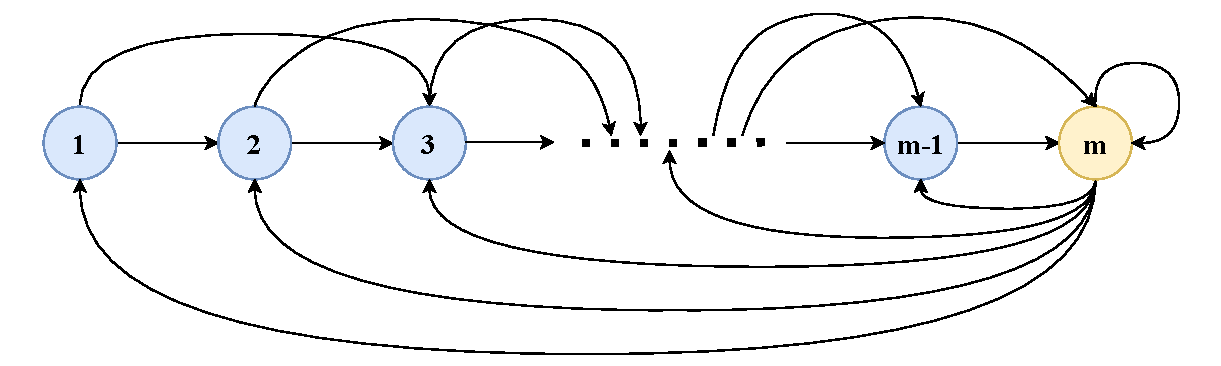
\includegraphics[width=0.7\textwidth]{img/boyan.pdf}
    \caption{Boyan's Chain of $m$ States}
    \label{fig:boyan chain}
\end{figure}
\begin{algorithm}
    \caption{Boyan Chain MRP and Feature Generation (Non-Representable)} \label{alg:boyan generation}
    \begin{algorithmic}[1]
    \STATE \textbf{Input:} state space size $m = \abs{\fS}$, feature dimension $d$ 
    \FOR{$s \in \fS$}
    \STATE $\phi(s) \sim \uniform{(-1, 1)^d}$ \CommentSty{\, // feature}
    \ENDFOR
    \STATE $p_0 \sim \uniform{(0, 1)^m}$ \CommentSty{\, // initial distribution}
    \STATE $p_0 \gets p_0 /\sum_s p_0(s)$ 
    \STATE $r \sim \uniform{(-1, 1)^m}$ \CommentSty{\, // reward function}
    \STATE $p \gets 0_{m \times m}$ \CommentSty{\, // transition function}
    \FOR{$i = 1, \dots, m - 2 $}
        \STATE $\epsilon \sim \uniform{(0, 1)}$
        \STATE $p(i, i+1)$ $\gets$ $\epsilon$
        \STATE $p(i, i+2)$ $\gets$ $1 - \epsilon$
    \ENDFOR
    \STATE $p(m-1, m)$ $\gets$ 1
    \STATE $z$ $\gets$ $\uniform{(0, 1)^m}$
    \STATE $z$ $\gets$ $z/\sum_s z(s)$
    \STATE $p(m, 1:m)$ $\gets$ $z$
    \STATE \textbf{Output:} MRP $(p_0, p, r)$ and feature map $\phi$
    \end{algorithmic}
\end{algorithm}

\tb{Representable Value Function.}
With the above sampling procedure,
there is no guarantee that the true value function $v$ is always representable by the features.
In other words,
there is no guarantee that there exists a $w \in \R^d$ satisfying $v(s) = \indot{w}{\phi(s)}$ for all $s \in \fS$.
Most of our experiments use this setup.
It is,
however,
also beneficial sometimes to work with evaluation tasks where the true value function is guaranteed to be representable.
Algorithm~\ref{alg:boyan generation representable} achieves this by randomly generating a $w_*$ first and compute $v(s) \doteq \indot{w_*}{\phi(s)}$.
The reward is then analytically computed as $r \doteq (I_m - \gamma p) v$.
We recall that in the above, we regard $p$ as a matrix in $\R^{m \times m}$.

% As noted earlier, the rewards and states sampled in Algorithm \ref{alg:boyan generation} may result in a ground truth value function $v(s)$ that is not representable. In Appendix \ref{appendix: nonlinear}, we compare nonlinear transformers with batch TD. Most experiments use Algorithm \ref{alg:boyan generation} to generate trajectories; however, we also conduct an experiment comparing these methods when the value function is representable by a linear model. Here, we detail the Markovian trajectory generation procedure for ensuring the value function is representable.

% To achieve this, instead of randomly sampling a reward function directly, we first randomly sample a ground truth weight $w^*\in \R^d$ from $\qty[-1,1]^d$.  and Then we compute the ground truth value function $v\in \R^m$ where $v(s) = \indot{w^*}{\phi(s)}$ for each $s \in \fS$. Using the same process as described in the previous section, we sample the transition dynamics of the MRP $P$. Then we can compute the reward function $r \in \R^m$ that will result in $v(s)$ for this MRP using $r=\qty(I_m - \gamma P)v$.

\begin{algorithm}[h]
    \caption{Boyan Chain MRP and Feature Generation (Representable)} \label{alg:boyan generation representable}
    \begin{algorithmic}[1]
    \STATE \textbf{Input:} state space size $m = \abs{\fS}$, feature dimension $d$, discount factor $\gamma$
    \STATE $w^* \sim \uniform{(-1, 1)^d}$ \CommentSty{\, // ground-truth weight}
    \FOR{$s \in \fS$}
    \STATE $\phi(s) \sim \uniform{(-1, 1)^d}$ 
    \CommentSty{\, // feature}
    \STATE $v(s) \gets \indot{w^*}{\phi(s)}$ \CommentSty{\, // ground-truth value function}
    \ENDFOR
    \STATE $p_0 \sim \uniform{(0, 1)^m}$ \CommentSty{\, // initial distribution}
    \STATE $p_0 \gets p_0 /\sum_s p_0(s)$
    \STATE $p \gets 0_{m \times m}$ \CommentSty{\, // transition function}
    \FOR{$i = 1, \dots, m - 2 $}
        \STATE $\epsilon \sim \uniform{(0, 1)}$
        \STATE $p(i, i+1)$ $\gets$ $\epsilon$
        \STATE $p(i, i+2)$ $\gets$ $1 - \epsilon$
    \ENDFOR
    \STATE $p(m-1, m)$ $\gets$ 1
    \STATE $z$ $\gets$ $\uniform{(0, 1)^m}$
    \STATE $z$ $\gets$ $z/\sum_s z(s)$
    \STATE $p(m, 1:m)$ $\gets$ $z$
    \STATE $r \gets \qty(I_m - \gamma p)v$ \CommentSty{\, // reward function}
    \STATE \textbf{Output:} MRP $(p_0, p, r)$ and feature map $\phi$
    \end{algorithmic}
\end{algorithm}

\newpage

\section{Additional Experiments with Linear Transformers} \label{appendix: additional linear}
\subsection{Experiment Setup} \label{appendix: experiment setup}
% In this section, we detail our experimental setup for training transformers following Algorithm \ref{deep td}. To generate the Markovian trajectories used in our training samples, we utilize the Boyan Chain MRP  with a state space size of $|\mathcal{S}|=10$ as depicted in Figure~\ref{fig:boyan chain} \citep{boyan1999least}. 
%each state $i$, except for the last two states $m-1, \ m$, transitions to its immediate two successors, $i+1$ and $i+2$.
%    To ensure diversity during training, each time we sample a new Boyan Chain MRP, we randomly sample the feature vectors, reward functions, and the transition matrix, thereby ensuring with high probability that the transformer never sees the same MRP twice. We present our complete Markovian Trajectory Procedure in Algorithm \ref{alg:boyan generation} in Appendix \ref{appendix: Markovian Trajectory}.

We use Algorithm~\ref{alg:boyan generation} as $d_\text{task}$ for the experiments in the main text with Boyan's chain of 10 states.
In particular, 
we consider a context of length $n=30$, feature dimension $d=4$, and utilize a discount factor $\gamma = 0.9$. In Section \ref{sec: transformers do implement TD(0)}, we consider a 3-layer transformer ($L=3$), but additional analyses on the sensitivity to the number of transformer layers ($L$) and results from a larger scale experiment with $d=8, n=60,$ and $|\mathcal{S}|=20$ are presented in \ref{appendix: autoregressive experiments}. We also explore non-autoregressive (i.e., "sequential") layer configurations in \ref{appendix: sequential linear}.

When training our transformer, we utilize an Adam optimizer ~\citep{kingma2014adam} with an initial learning rate of $\alpha = 0.001$ and weight decay rate of $1\times 10^{-6}$. $P_0$ and $Q_0$ are randomly initialized using Xavier initialization with a gain of $0.1$. 
We trained our transformer on $k=4000$ different evaluation tasks.
For each task, we generated a trajectory of length $\tau = 347$, resulting in $\tau - n -2 = 320$ transformer parameter updates.

Since the models in these experiments are small ($\sim 10$ KB), we did not use any GPU during our experiments. We trained our transformers on a standard Intel i9-12900-HK CPU, and training each transformer took $\sim20$ minutes.

For implementation\footnote{The code will be made publicly available upon publication.}, we used NumPy~\citep{harris2020numpy} to process the data and construct Boyan's chain, PyTorch~\citep{ansel2024pytorch} to define and train our models, and Matplotlib~\citep{hunter2007matplotlib} plus SciencePlots~\citep{garrett2021SciencePlots} to generate our figures.

\subsubsection{Trained Transformer Element-wise Convergence Metrics} \label{appendix: element-wise metrics}
To visualize the parameters of the linear transformer trained by Algorithm \ref{deep td}, we report element-wise metrics. For $P_0$, we report the value of its bottom-right entry, which, as noted in \eqref{eq: Z_0 P Q TD define}, should approach one if the transformer is learning to implement TD. The other entries of $P_0$ should remain close to zero. Additionally, we report the average absolute value of the elements of $P_0$, excluding the bottom-right entry, to check if these elements stay near zero during training.

For $Q_0$, we recall from \eqref{eq: Z_0 P Q TD define} that if the transformer learned to implement normal batch TD, the upper-left $d\times d$ block of the matrix should converge to some $-I_d$, while the upper-right $d\times d$ block (excluding the last column) should converge to $I_d$. To visualize this, we report the trace of the upper-left $d\times d$ block and the trace of the upper-right $d\times d$ block (excluding the last column). The rest of the elements of $Q_0$ should remain close to 0, and to verify this, we report the average absolute value of the entries of $Q_0$, excluding the entries that were utilized in computing the traces. 

Since, $P_0$ and $Q_0$ are in the same product in~\eqref{eq linear attention} we sometimes observe during training that $P_0$ converges to $-P_0^{\td}$ and $Q_0$ converges to $-Q_0^{\td}$ simultaneously. When visualizing the matrices,  we negate both $P_0$ and $Q_0$ when this occurs.

It's also worth noting that in Theorem \ref{thm: TD(0)} we prove a $L$-layer transformer parameterized as in \eqref{eq: Z_0 P Q TD define} with $C_0 = I_d$ implements $L$ steps of batch TD exactly with a fixed update rate of one. However, the transformer trained using Algorithm \ref{deep td} could learn to perform $\td$ with an arbitrary learning rate ($\alpha$ in~\eqref{eq: linear td(0)}). Therefore, even if the final trained $P_0$ and $Q_0$ differ from their constructions in \eqref{eq: Z_0 P Q TD define} by some scaling factor, the resulting algorithm implemented by the trained transformer will still be implementing TD.
In light of this,
we rescale $P_0$ and $Q_0$ before visualization.
In particular, we divide $P_0$ and $Q_0$ by the maximum of the absolute values of their entries, respectively, such that they both stay in the range $[-1, 1]$ after rescaling.

\subsubsection{Trained Transformer and Batch TD Comparison Metrics} \label{appendix: comparison metrics}
To compare the transformers with batch TD we report several metrics following \citet{vonoswald2023transformers, akyurek2023learning}. 
Given a context $C \in \R^{(2d+1) \times n}$ and a query $\phi \in \R^d$,
we construct the prompt as
\begin{align}
    Z^{(\phi, C)} \doteq \mqty[C & \mqty[\phi \\ 0_{d \times 1} \\ 0]].
\end{align}
We will suppress the context $C$ in subscript when it does not confuse.
We use $Z^{(s)} \doteq Z^{(\phi(s))}$ as shorthand.
% Given some state $s \in \fS$, we define $q(s): \fS \to \R^{2d+1} \doteq \mqty[\phi(s)^\top & 0_{1\times(d+1)}]^\top$.
% We first define a function $q$,
% which is used to construct the query for states,
% as
% \begin{align}
    % s \in \fS \mapsto q(s) \doteq \mqty[\phi(s) \\ 0_{d \times 1} \\ 0] \in \R^{(2d + 1)}.
% \end{align}
% Assuming we have a fixed context $C$,
% we define the prompt $Z_0^{(s)}$ with context $C$ and query state $s$ as
% $Z_0^{(s)} \doteq \mqty[C & q(s)]$. 
We use $d_p$ to denote the stationary distribution of the MRP with transition function $p$
and assume the context $C$ is constructed based on trajectories sampled from this MRP.
Then, we can define $v_{\theta} \in \R^{\abs{\fS}}$, where $v_{\theta}(s) \doteq \tf_L(Z_0^{(s)}; \theta)$ for each $s \in \mathcal{S}$.
Notably,
$v_\theta$ is then the value function estimation induced by the transformer parameterized by $\theta \doteq \qty{(P_l, Q_l)}$ given the context $C$.
In the rest of the appendix,
we will use $\theta_\tf$ as the learned parameter from Algorithm~\ref{deep td}.
As a result, $v_\tf \doteq v_{\theta_\tf}$ denotes the learned value function.
% We note that $v_{\theta}$ is the estimated value function for the learned transformer $\tf_L$ given context $C$.

We define $\theta_\td \doteq \qty{(P_l^\td, Q_l^\td)}_{l=0,\dots, L-1}$ with $C_l = \alpha I$ (see~\eqref{eq: Z_0 P Q TD define}) and
\begin{align}
    v_\td(s) \doteq \tf_L(Z_0^{(s)}; \theta_\td).
\end{align}
In light of Theorem~\ref{thm: TD(0)},
$v_\td$ is then the value function estimation obtained by running the batch TD algorithm~\eqref{eq: TD(0) w_update} on the context $C$ for $L$ iterations,
using a constant learning rate $\alpha$.

We would like to compare the two functions $v_\tf$ and $v_\td$ to future examine the behavior of the learned transformers.
However,
$v_\td$ is not well-defined yet because it still has a free parameter $\alpha$,
the learning rate.
% We recall that in Theorem~\ref{thm: TD(0)}, $C_l$ is arbitrary.
% In particular, if $C_l = \alpha I$,
% then the transformer with 
% It is informative to compare the two value functions.
% We use $\tf^{\td}_L$ to denote the transformer parameterized as in~\eqref{eq: Z_0 P Q TD define}, 
% and we use  $\theta_{\td} \doteq \qty{P_l, Q_l}_{l=0,1,\dots,L-1}$ to refer its fixed parameters.
% Therefore, we can similarly define the value function for Batch TD $v_{\td} \in \R^{\abs{\fS}}$, where $v_{\td}(s_i) \doteq \tf^{\td}_L(Z_0^{(s_i)}, \theta_{\td})$ for each $s_i \in \mathcal{S}$.
% As mentioned in Appendix \ref{appendix: element-wise metrics} while $\tf^{\td}_L$ has a fixed learning rate $\frac{1}{n}$, the transformer trained using Algorithm \ref{deep td} could learn to perform TD with an arbitrary learning rate ($\alpha$ in~\eqref{eq: linear td(0)}). The discrepancy between the TD update rates poses a challenge for us to functionally compare $\tf_L$ and $\tf_L^{\td}$ because the TD errors and the final value functions learned by $\tf_L$ and $\tf_L^{\td}$ will likely differ for different learning rates, even if they are implementing the same algorithm. 
%This phenomenon is demonstrated in Figure \ref{fig:parameter convergence auto} where we see that the learned $P$ matrix converges 
%Our hypothesis is that the parameters of the transformers trained according to Algorithm \ref{} will converge to $\theta_{\td}$ up to some scaling factor.
%We interpret this scaling factor as the optimized TD update rate discovered by the transformers during training, given their limited numbers of layers.
\cite{vonoswald2023transformers} resolve a similar issue in the in-context regression setting 
via using a line search to find the (empirically) optimal $\alpha$.
% this issue in their regression task via a line search over the learning rates to find the best candidate.
Inspired by \cite{vonoswald2023transformers},
we also aim to find the empirically optimal $\alpha$ for $v_\td$.
% Here, we remedy this problem by making the update rate a trainable parameter for $\tf_L^{\td}$.
We recall that $v_\td$ is essentially the transformer $\tf_L(Z_0^{(s)}; \theta_\td)$ with only 1 single free parameter $\alpha$.
We then train this transformer with Algorithm~\ref{deep td}. 
We observe that $\alpha$ quickly converges and use the converged $\alpha$ to complete the definition of $v_\td$.
We are now ready to present different metrics to compare $v_\tf$ and $v_\td$.
We recall that both are dependent on the context $C$.

% Denoting the update rate by $\alpha$, that means \eqref{eq: Z_l update} becomes
% \begin{align}
%     Z_{l+1} = Z_l + \frac{\alpha}{n} \attn_{P_l, Q_l}(Z_l)
% \end{align}
% for $\tf_L^{\td}$.
% With fixed $\theta_{\td}$, we train the update rate of $\tf_L^{\td}$ via semi-gradient TD concurrently with $\tf_L$.
% We observe the update rate quickly converges and assume it matches that of the fully-trainable $\tf_L$.

\tb{Value Difference (VD).}
First, for a given context $C$, 
we compute the Value Difference (VD) to measure the difference between the value function approximated by the trained transformer and the value function learned by batch TD, 
weighted by the stationary distribution.
To this end, we define,
\begin{align}
    \text{VD}(v_\tf, v_\td) \doteq \norm{v_\tf - v_\td}_{d_p}^2,
\end{align}
We recall that $d_p \in \R^\ns$ is the stationary distribution of the MRP, and the weighted $\ell_2$ norm is defined as $\norm{v}_d \doteq \sqrt{\sum_s v(s)^2 d(s)}$.

\tb{Implicit Weight Similarity (IWS).}
We recall that $v_\td$ is a linear function, i.e., $v_\td(s) = \indot{w_L}{\phi(s)}$ with $w_L$ defined in Theorem~\ref{thm: TD(0)}.
We refer to this $w_L$ as $w_\td$ for clarity.
The learned value function $v_\tf$ is, however, not linear even with a linear transformer.
Following \citet{akyurek2023learning},
we compute the best linear approximation of $v_\tf$.
In particular,
given a context $C$,
we define
\begin{align}
    w_\tf \doteq \arg\min_w \norm{\Phi w - v_\tf}_{d_p}. 
\end{align}
Here $\Phi \in \R^{\ns \times d}$ is the feature matrix,
each of which is $\phi(s)^\top$.
Such a $w_\tf$ is referred to as implicit weight in \citet{akyurek2023learning}.
Following \citet{akyurek2023learning},
we define 
\begin{align}
    \text{IWS}(v_\tf, v_\td) \doteq d_\text{cos}(w_\tf, w_\td)
\end{align}
to measure the similarity between $w_\tf$ and $w_\td$.
Here $d_\text{cos}(\cdot, \cdot)$ computes the cos similarity between two vectors.

%  (see Theorem~\ref{thm: TD(0)}).
% We recall that both $v_\theta$ and $v_\td$ can be regarded as a function that maps the context $C$ to a value function estimate in $\R^\ns$.
% Given a context $C$, if $\tf_L$ indeed implements batch TD with a similar update rate, then we expect $v_{\theta} \approx v_\td$ for any $C$.
% We call the similarity between $v_{\theta}$ and $v_\td$ zero-order similarity to reflect the fact the metric does not take any gradient term into consideration.
% During training, both $v_{\theta}$ and $v_\td$ can be noisy, making a direct comparison less informative.
% In light of this, we resort to a different approach that mitigates this issue.
% Since $v_\td$ is the value function learned by batch TD with linear function approximation, we can find the weight $w_\td \in \R^d$, such that
% \begin{align}
%     v_\td = \Phi w_\td.
% \end{align}
% where $\Phi \in \R^{|\fS| \times d}$ is the feature matrix.
% The value function $v_{\theta}$ may not lie exactly within the column space of $\Phi$.
% Similar to ~, we therefore use the weight of the best linear model as its implicit weight, defined as
% \begin{align}
%     w_\tf \doteq \arg \min_w \norm{v_{\theta} - \Phi w}_D.
% \end{align}
% We then compare $w_\td$ with $w_\tf$ using their cosine similarity, as a proxy to comparing $v_\td$ and $v_{\theta}$.
%\begin{align}
%    \text{cos sim}(w_\td, w_\tf) \doteq \frac{w_\td^\top w_\tf}{\norm{w_\td}\norm{w_\tf}}. 
%\end{align}

\tb{Sensitivity Similarity (SS).} 
Recall that $v_{\tf}(s) = \tf_L(Z_0^{(s)}; \theta_\tf)$ and $v_{\td}(s) = \tf_L(Z_0^{(s)}; \theta_{\td})$. 
In other words, given a context $C$,
both $v_\tf(s)$ and $v_\td(s)$ are functions of $\phi(s)$.
Following \citet{vonoswald2023transformers},
we then measure the sensitivity of $v_\tf(s)$ and $v_\td(s)$ w.r.t. $\phi(s)$.
This similarity is easily captured by gradients.
% Define
% \begin{align}
%     Z_0^{(\phi)} \doteq \mqty[C & \mqty[\phi \\ 0_{d\times 1} \\ 0]].
% \end{align}
% The desired sensitivity is then captured by $\eval{\nabla_{\phi} \tf_L(Z_0^{(\phi)}; \theta_\tf)}_{\phi = \phi(s)}$ and $\eval{\nabla_{\phi} \tf_L(Z_0^{(\phi)}; \theta_\td)}_{\phi = \phi(s)}$.
In particular, 
we define
\begin{align}
    \text{SS}(v_\tf, v_\td) \doteq \sum_s d_p(s) d_\text{cos}\left(\eval{\nabla_{\phi} \tf_L(Z_0^{(\phi)}; \theta_\tf)}_{\phi = \phi(s)}, \eval{\nabla_{\phi} \tf_L(Z_0^{(\phi)}; \theta_\td)}_{\phi = \phi(s)}\right).
\end{align}
Notably,
it trivially holds that
\begin{align}
    w_\td = \eval{\nabla_{\phi} \tf_L(Z_0^{(\phi)}; \theta_\td)}_{\phi = \phi(s)}.
\end{align}

We note that the element-wise convergence of learned transformer parameters (e.g., Figure~\ref{fig: linear attention parameters auto l=3}) is the most definite evidence for the emergence of in-context TD.
The three metrics defined in this section are only auxiliary when linear attention is concerned.
That being said,
\tb{the three metrics are important when nonlinear attention is concerned}.

% We can write $\nabla_{\phi_s} \tf_L(Z_0^{(s)}, \theta)$ to denote the gradient of the transformer with respect to the query state $\phi_s$, which is referred to as the "sensitivity" in the literature . The sensitivity yields the explicit models computed by the algorithm. Since we proved in Theorem \ref{thm: TD(0)} that $\tf^{\td}_L(Z_0^{(s)}, \theta_{\td}) = \indot{w}{\phi}$, we have that $\nabla_\phi \tf^{\td}_L(Z_0^{(s)}, \theta_{\td}) = w_{\td}$. We compare the cosine similarity of the sensitivities weighted by the stationary distribution using,
% \begin{align}
%     \E_{s\sim d_{p}} \left[\text{cos sim}\left(\nabla_{\phi_s} \tf_L(Z_0^{(s)}, \theta), \nabla_\phi \tf^{\td}_L(Z_0^{(s)}, \theta_{\td})\right)\right] \\
%     = \sum_{s \in \mathcal{S}} d_p(s) \text{cos sim}\left(\nabla_{\phi_s} \tf_L(Z_0^{(s)}, \theta), \nabla_\phi \tf^{\td}_L(Z_0^{(s)}, \theta_{\td})\right).
% \end{align}
%  Because we lack direct access to the initial parameters $\theta$ of the trained transformer, we cannot expect the models to agree exactly.

\subsection[Autoregressive Linear Transformers with L = 1, 2, 3, 4 Layers]{Autoregressive Linear Transformers with $L=1,2,3,4$ Layers} \label{appendix: autoregressive experiments}
In this section,
we present the experimental results for autoregressive linear transformers with different numbers of layers. 
In Figure \ref{fig: linear parameter convergence auto l=1,2,4}, we present the element-wise convergence metrics for autoregressive transformers with $L=1,2,4$ layers.
The plot with $L = 3$ is in Figure~\ref{fig: linear parameter convergence auto l=3} in the main text.
% ~\ref{fig: linear attention metrics auto l=3} 
We can see that for the $L=1$ case, $P_0$ and $Q_0$ converge to the construction in Corollary \ref{cor one layer},
which, as proved, implements TD(0) in the single layer case.  
For the $L=2,4$ cases, we see that $P_0$ and $Q_0$ converge to the construction in Theorem \ref{thm: TD(0)}. 
We also observe that as the number of transformer layers $L$ increases,
the learned parameters are more aligned with the construction of $P_0^{\td}$ and $Q_0^{\td}$ with $C_0=I$.
%  from ~\eqref{eq: Z_0 P Q TD define} that implements normal batch TD.
\begin{figure}[htbp]
    \centering
    \begin{subfigure}[b]{0.39\textwidth}
        \centering
        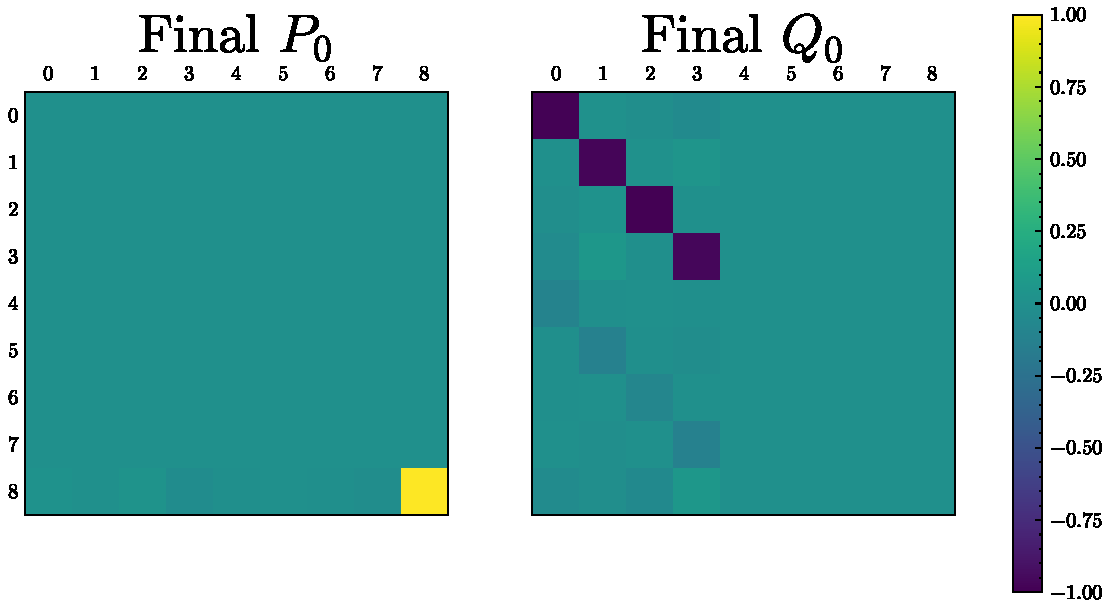
\includegraphics[width=\textwidth]{img/linear/1layer/PQ_mean_1_4000.pdf}
        \caption{Learned $P_0$ and $Q_0$ with $L=1$}
        \label{fig: linear attention parameters auto l=1}
    \end{subfigure}
    \begin{subfigure}[b]{0.6\textwidth}
        \centering
        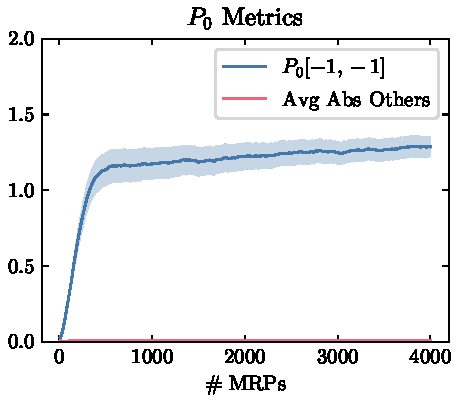
\includegraphics[width=0.4\textwidth]{img/linear/1layer/P_metrics_1.pdf}
        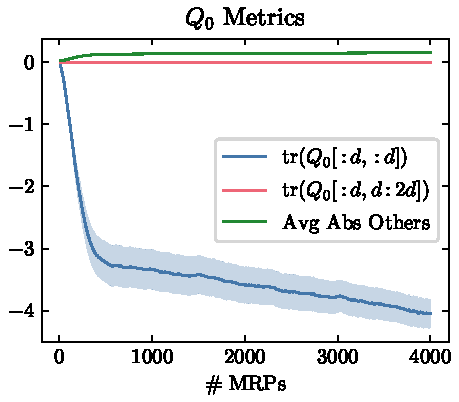
\includegraphics[width=0.4\textwidth]{img/linear/1layer/Q_metrics_1.pdf}
        \caption{Element-wise learning progress of $P_0$ and $Q_0$}
        \label{fig: linear attention metrics auto l=1}
    \end{subfigure}
    \begin{subfigure}[b]{0.39\textwidth}
        \centering
        
\includegraphics[width=\textwidth]{img/linear/2layers/PQ_mean_1_4000.pdf}
        \caption{Learned $P_0$ and $Q_0$ with $L=3$}
        \label{fig: linear attention parameters auto l=2}
    \end{subfigure}
    \begin{subfigure}[b]{0.6\textwidth}
        \centering
        
\includegraphics[width=0.4\textwidth]{img/linear/2layers/P_metrics_1.pdf}
        
\includegraphics[width=0.4\textwidth]{img/linear/2layers/Q_metrics_1.pdf}
        \caption{Element-wise learning progress of $P_0$ and $Q_0$}
        \label{fig: linear attention metrics auto l=2}
    \end{subfigure}
    \begin{subfigure}[b]{0.39\textwidth}
        \centering
        
\includegraphics[width=\textwidth]{img/linear/4layers/PQ_mean_1_4000.pdf}
        \caption{Learned $P_0$ and $Q_0$ with $L=4$}
        \label{fig: linear attention parameters auto l=4}
    \end{subfigure}
    \begin{subfigure}[b]{0.6\textwidth}
        \centering
        
\includegraphics[width=0.4\textwidth]{img/linear/4layers/P_metrics_1.pdf}
        
\includegraphics[width=0.4\textwidth]{img/linear/4layers/Q_metrics_1.pdf}
        \caption{Element-wise learning progress of $P_0$ and $Q_0$}
        \label{fig: linear attention metrics auto l=4}
    \end{subfigure}
    \caption{
    Visualization of the learned \tb{autoregressive} transformers and the learning progress.
    Averaged across 30 seeds and the shaded region denotes the standard errors.
    See Appendix \ref{appendix: element-wise metrics} for details about normalization of $P_0$ and $Q_0$ before visualization.
    }
        % Visualization of the learned linear autoregressive transformers and their learning progress. Left: $P_0$ and $Q_0$ scaled to $[-1, 1]$ with (a) $L=1$, (c) $L=2$, and (e) $L=4$ layers. 
    % Right: Metrics monitoring $P_0$ and $Q_0$ element-wise throughout training with (b) $L=1$, (d) $L=2$, and (f) $L=4$ Layers. All figures report the average across 30 seeds and the shaded regions in (b), (d) and (f) denote the standard errors. Note that the $L=3$ layer case is presented in section \ref{sec: transformers do implement TD(0)}.}
    \label{fig: linear parameter convergence auto l=1,2,4}
\end{figure}

We also present the comparison of the learned transformer with batch TD according to the metrics described in Appendix \ref{appendix: comparison metrics}. 
In Figure \ref{fig:linear batch td comparison}, 
we present the value difference,
implicit weight similarity,
and sensitivity similarity.
In Figures \ref{fig: error metrics linear auto l=1} -- \ref{fig: error metrics linear auto l=4}, we present the results for different transformer layer numbers $L=1,2,3,4$. In Figure \ref{fig: error metrics linear auto l=3 larger}, 
we present the metrics for a 3-layer transformer, but we increase the feature dimension to $d=8$ and also the context length to $n=60$. 

In all instances, we see a strong similarity between the trained linear transformers and batch TD. 
We see that the cosine similarities of the sensitivities are near one, 
as are the implicit weight similarities. 
Additionally, the value difference 
% between the value function learned by the trained transformer and the value function learned by batch TD 
approaches zero during training. 
This further demonstrates that the autoregressive linear transformers trained according to Algorithm \ref{deep td} learn to implement TD(0).

\begin{figure}[htbp]
  \centering
  \begin{subfigure}{0.32\textwidth}
    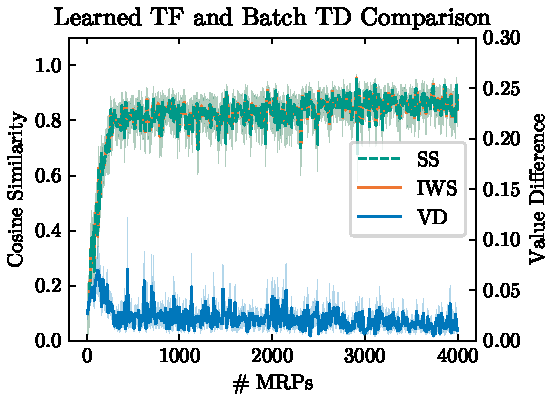
\includegraphics[width=\textwidth]{img/linear/1layer/cos_similarity.pdf}
    \caption{$L=1$}
    \label{fig: error metrics linear auto l=1}
  \end{subfigure}
  \begin{subfigure}{0.32\textwidth}
    
\includegraphics[width=\textwidth]{img/linear/2layers/cos_similarity.pdf}
    \caption{$L=2$}
    \label{fig: error metrics linear auto l=2}
  \end{subfigure}
\begin{subfigure}{0.32\textwidth}
    
\includegraphics[width=\textwidth]{img/linear/standard/cos_similarity.pdf}
    \caption{$L=3$}
    \label{fig: error metrics linear auto l=3}
  \end{subfigure}
  \begin{subfigure}{0.32\textwidth}
    
\includegraphics[width=\textwidth]{img/linear/4layers/cos_similarity.pdf}
    \caption{$L=4$}
    \label{fig: error metrics linear auto l=4}
  \end{subfigure}
  \begin{subfigure}{0.32\textwidth}
      
\includegraphics[width=\textwidth]{img/linear/large/cos_similarity.pdf}
      \caption{$L=3$ ($d=8, \ n=60$)}
    \label{fig: error metrics linear auto l=3 larger}
  \end{subfigure}
  \caption{Value difference (VD), implicit weight similarity (IWS), and sensitivity similarity (SS) between the learned \tb{autoregressive} transformers and batch TD with different layers.
  All curves are averaged over 30 seeds and the shaded regions are the standard errors.}
  \label{fig:linear batch td comparison}
\end{figure}


\subsection[Sequential Transformers with L = 2, 3, 4 Layers]{Sequential Transformers with $L=2,3,4$ Layers} 
\label{appendix: sequential linear}
So far, we have been using linear transformers with one parametric attention layer applied repeatedly for $L$ steps to implement an $L$-layer transformer.
Another natural architecture in contrast with the autoregressive transformer is a sequential transformer with $L$ distinct attention layers, where the embedding passes over each layer exactly once during one pass of forward propagation.

In this section, we repeat the same experiments we conduct on the autoregressive transformer with sequential transformers with $L = 2, 3, 4$ as their architectures coincide when $L=1$.
We compare the sequential transformers with batch TD(0) and report the three metrics 
in Figure~\ref{fig: error metrics linear seq}.
We observe that the implicit weight similarity and the sensitivity similarity grow drastically to near 1, 
and the value difference drops considerably after a few hundred MRPs for all three layer numbers.
It suggests that sequential transformers trained via Algorithm~\ref{deep td} are functionally close to batch TD.
% With fewer layers, the curves change faster but tend to be noisier.
% We reason that deeper transformers have more parameters and thus require more samples to converge.

Figure~\ref{fig: linear parameter convergence seq L=3} shows the visualization of the converged $\qty{P_l, Q_l}_{l=0,1,2}$ of a 3-layer sequential linear transformer and their element-wise convergence.
Sequential transformers exhibit very special patterns in their learned weights.
We see that the input layer converges to a pattern very close to our configuration in Theorem~\eqref{thm: TD(0)}.
However, the deeper the layer, we observe the more the diagonal of $Q_l[1:d, d+1:2d]$ fades.
The $P$ matrices, on the other hand, follow our configuration closely, especially for the final layer.
We speculate this pattern emerges because sequential transformers have more parametric attention layers and thus can assign a slightly different role to each layer but together implement batch TD(0) as suggested by the black-box functional comparison in Figure~\ref{fig: error metrics linear seq}.
\begin{figure}[htbp]
  \centering
  \begin{subfigure}{0.32\textwidth}
    
\includegraphics[width=\textwidth]{img/linear/sequential_2layers/cos_similarity.pdf}
    \caption{$L=2$}
    \label{fig: error metrics linear seq l=2}
  \end{subfigure}
  \begin{subfigure}{0.32\textwidth}
    
\includegraphics[width=\textwidth]{img/linear/sequential/cos_similarity.pdf}
    \caption{$L=3$}
    \label{fig: error metrics linear seq l=3}
  \end{subfigure}
  \begin{subfigure}{0.32\textwidth}
    
\includegraphics[width=\textwidth]{img/linear/sequential_4layers/cos_similarity.pdf}
    \caption{$L=4$}
    \label{fig: error metrics linear seq l=4}
  \end{subfigure}
  \caption{
Value difference (VD), implicit weight similarity (IWS), and sensitivity similarity (SS) between the learned \tb{sequential} transformers and batch TD with different layers.
  All curves are averaged over 30 seeds, and the shaded regions are the standard errors.
    % Sensitivity cosine similarity, 0-th order cosine similarity, and MSVE with respect to batch TD(0) for (a) $L=2$, (b) $L=3$, and (c) $L=4$ layer sequential transformers. All figures are averaged across 30 seeds and the shaded regions denote the standard errors.
    }
  \label{fig: error metrics linear seq}
\end{figure}

\begin{figure}[htbp]
    \centering
    \begin{subfigure}{0.39\textwidth}
        \centering
        
\includegraphics[width=\textwidth]{img/linear/sequential/PQ_mean_1_4000.pdf}
        \caption{Learned $P_0$ and $Q_0$}
        \label{fig: linear attention parameters seq l=0}
    \end{subfigure}
    \begin{subfigure}{0.6\textwidth}
        \centering
        
\includegraphics[width=0.4\textwidth]{img/linear/sequential/P_metrics_1.pdf}
        
\includegraphics[width=0.4\textwidth]{img/linear/sequential/Q_metrics_1.pdf}
        \caption{Element-wise learning progress of $P_0$ and $Q_0$}
        \label{fig: linear attention metrics seq l=0}
    \end{subfigure}
    \begin{subfigure}{0.39\textwidth}
        \centering
        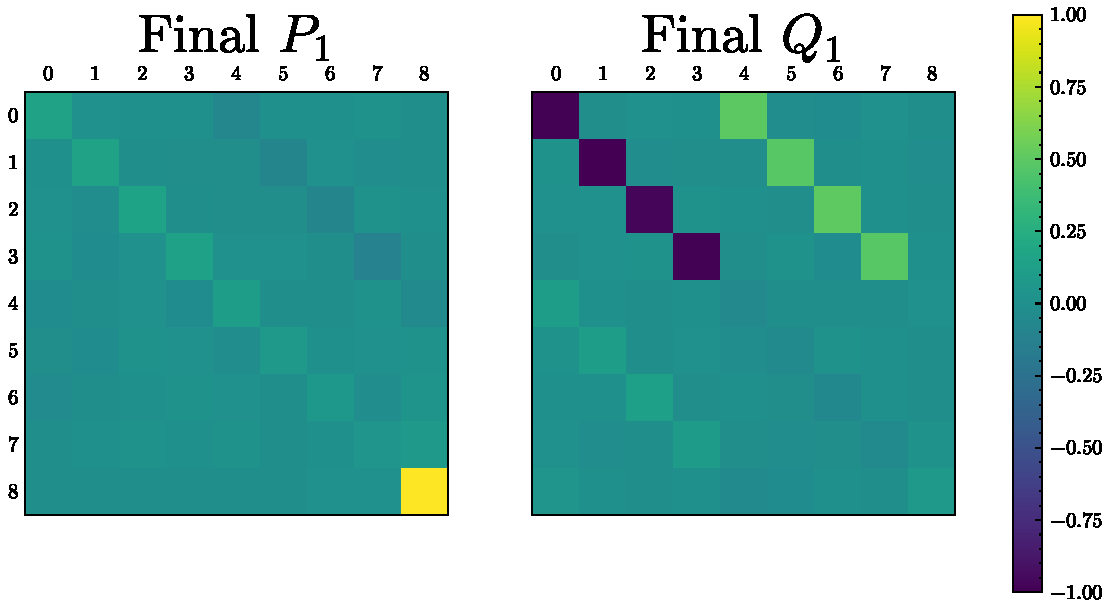
\includegraphics[width=\textwidth]{img/linear/sequential/PQ_mean_2_4000.pdf}
        \caption{Learned $P_1$ and $Q_1$}
        \label{fig: linear attention parameters seq l=1}
    \end{subfigure}
    \begin{subfigure}{0.6\textwidth}
        \centering
        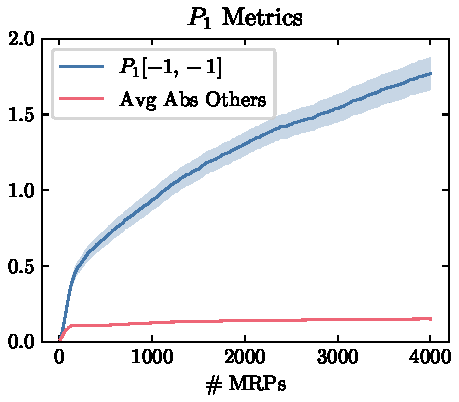
\includegraphics[width=0.4\textwidth]{img/linear/sequential/P_metrics_2.pdf}
        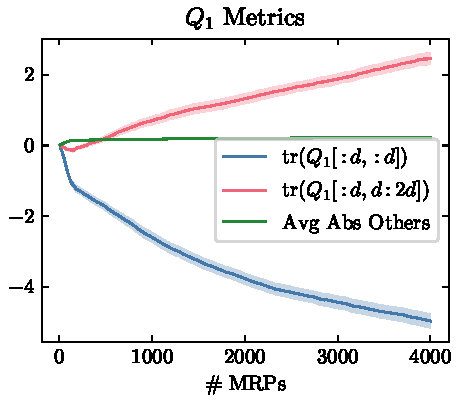
\includegraphics[width=0.4\textwidth]{img/linear/sequential/Q_metrics_2.pdf}
        \caption{Element-wise learning progress of $P_1$ and $Q_1$}
        \label{fig: linear attention metrics seq l=1}
    \end{subfigure}
    \begin{subfigure}{0.39\textwidth}
        \centering
        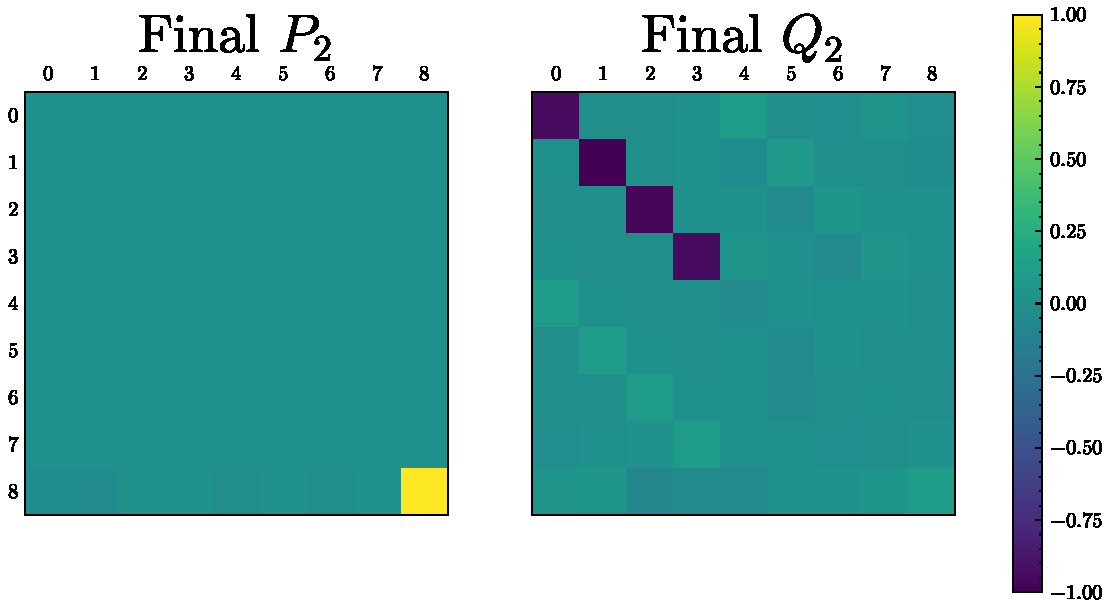
\includegraphics[width=\textwidth]{img/linear/sequential/PQ_mean_3_4000.pdf}
        \caption{Learned $P_2$ and $Q_2$}
        \label{fig: linear attention parameters seq l=2}
    \end{subfigure}
    \begin{subfigure}{0.6\textwidth}
        \centering
        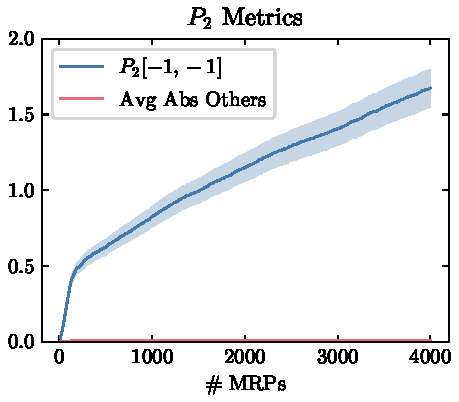
\includegraphics[width=0.4\textwidth]{img/linear/sequential/P_metrics_3.pdf}
        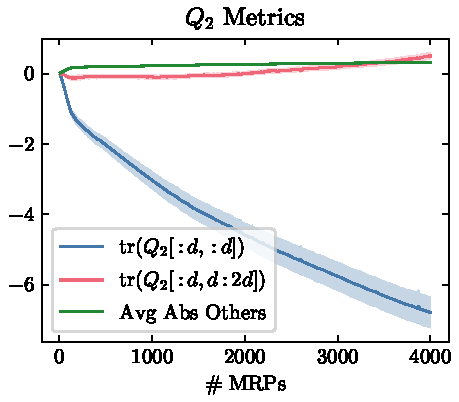
\includegraphics[width=0.4\textwidth]{img/linear/sequential/Q_metrics_3.pdf}
        \caption{Element-wise learning progress of $P_2$ and $Q_2$}
        \label{fig: linear attention metrics seq l=2}
    \end{subfigure}
    \caption{   Visualization of the learned $L=3$ \tb{sequential} transformers and the learning progress.
    Averaged across 30 seeds and the shaded region denotes the standard errors.
    See Appendix \ref{appendix: element-wise metrics} for details about normalization of $P_0$ and $Q_0$ before visualization.
    }
    \label{fig: linear parameter convergence seq L=3}
\end{figure}

\section{Nonlinear Attention}\label{appendix: nonlinear}
Until now, we have focused on only linear attention.
In this section,
we empirically investigate original transformers with the softmax function.
% The first part of our work studies linear transformer's ability to implement TD.
% In real world applications, transformers are mostly made nonlinear with multiple heads and layers.
% Thus, we investigate nonlinear transformers' ability to implement TD in-context in this section.
% We first consider the classic softmax activation used in \cite{vaswani2017}.
Given a matrix $Z$, 
we recall that self-attention computes its embedding as
\begin{align}
    \nattn(Z; P, Q) = PZM\softmax{Z^\top Q Z}.
\end{align}
Let $Z_l \in \R^{(2d+1)\times(n+1)}$ denote the input to the $l$-th layer, the output of an $L$-layer transformer with parameters $\qty{(P_l, Q_l)}_{l=0,\dots,L-1}$ is then computed as
\begin{align}
    \textstyle Z_{l+1} = Z_l + \frac{1}{n}\nattn(Z_l; P_l, Q_l)
    = Z_l + \frac{1}{n} PZM\softmax{Z^\top Q Z}.
\end{align}
Analogous to the linear transformer, we define
\begin{align}
\ntf_L \qty(Z_0; \qty{P_l, Q_l}_{l=0,1\dots,L-1}) \doteq -Z_L[2d + 1, n + 1].
\end{align}
As a shorthand, we use $\ntf_L(Z_0)$ to denote the output of the softmax transformers given prompt $Z_0$. 
We use the same training procedure (Algorithm \ref{deep td}) to train the softmax transformers. 
In particular,
we consider a 3-layer autoregressive softmax transformer.

% \subsection{Comparison of Trained Softmax Transformer with Batch TD}
Notably, the three metrics in Appendix~\ref{appendix: comparison metrics} apply to softmax transformers as well.
We still compare the learned softmax transformer with the linear batch TD in~\eqref{eq: TD(0) w_update}.
In other words, the $v_\td$ related quantities are the same, and we only recompute $v_\tf$ related quantities in Appendix~\ref{appendix: comparison metrics}.
As shown in Figure~\ref{fig:nonlinear nonrepresentable},
the value difference remains small, and the implicit weight similarity increases.
This suggests that the learned softmax transformer behaves similarly to linear batch TD.
% the implicit weight similarity between the learned softmax transformer and the linear batch TD are close,
% suggesting the best linear approximation of the learned softmax transformer is similar to linear batch TD.
The sensitivity similarity, however, drops.
This is expected.
The learned softmax transformer $\ntf_L$ is unlikely to be a linear function w.r.t. to the query while $v_\td$ is linear w.r.t. the query.
So their gradients w.r.t. the query are unlikely to match.
To further investigate this hypothesis,
we additionally consider evaluation tasks where the true value function is guaranteed to be representable (Algorithm~\ref{alg:boyan generation representable}) and is thus a linear function w.r.t. the state feature.
This provides more incentives for the learned softmax transformer to behave like a linear function.
As shown in Figure~\ref{fig:nonlinear representable},
the sensitivity similarity now increases.

\begin{figure}[t!]
  \centering
  \begin{subfigure}[b]{0.33\textwidth}
    
\includegraphics[width=\textwidth]{img/nonlinear/standard/cos_similarity.pdf}
    \caption{General Value Function}
    \label{fig:nonlinear nonrepresentable}
  \end{subfigure}
  \hspace{5 mm}
% \begin{subfigure}[b]{0.32\textwidth}
    % 
\includegraphics[width=\textwidth]{img/nonlinear/sequential/cos_similarity.pdf}
    % \caption{Sequential}
    % \label{fig:nonlinear sequential}
% \end{subfigure}
  \begin{subfigure}[b]{0.327\textwidth}
    
\includegraphics[width=\textwidth]{img/nonlinear/representable/cos_similarity.pdf}
    \caption{Representable Value Function}
    \label{fig:nonlinear representable}
  \end{subfigure}
    \caption{
Value difference (VD), implicit weight similarity (IWS), and sensitivity similarity (SS) between the learned softmax transformers and linear batch TD.
  All curves are averaged over 30 seeds, and the shaded regions are the standard errors.
        % Sensitivity cosine similarity, 0-th order cosine similarity, and MSVE with respect to batch TD(0) for 3-layer nonlinear transformers. (a) Autoregressive transformers (b) Sequential transformers (c) Autoregressive transformers where the ground-truth value function is representable. All figures report the average across 30 seeds and the shaded regions denote the standard errors.
    }
    \label{fig: cosine sim nonlinear}
\end{figure}

\section{Experiments with CartPole Environment} \label{appendix: cartpole}
In this section, we present additional experimental results demonstrating that in-context TD emerges after large-scale pretraining using Algorithm \ref{deep td} where $d_{\text{task}}$ is derived from the CartPole environment \citep{brockman2016openai}.
\subsection{CartPole Evaluation Task Generation}
 Recall that in the main text, as well as Appendix \ref{appendix: additional linear} and \ref{appendix: nonlinear}, the transformers are pre-trained with tasks drawn from $d_{\text{task}}$ based on Boyan's Chain (See Appendix \ref{appendix: Markovian Trajectory}). Here, we extend the analysis by introducing $d_{\text{task}}$ based on the CartPole environment. Figure \ref{fig: cartpole intro} provides an introduction to the CartPole environment.

Recall that an evaluation task is defined by the tuple $(p_0, p, r, \phi)$. 
In the canonical CartPole environment, the states are a vector $s \in \R^4$ where the entries are the current position of the cart, the velocity of the cart, the angle of the pole, and the angular velocity of the pole. 
In our experiments, the initial state distribution $p_0$ and environment transition dynamics $p(s'|s,a)$ are given by the standard CartPole equations (e.g. see \href{https://github.com/openai/gym/blob/master/gym/envs/classic\_control/cartpole.py}{OpenAI CartPole Github}). 
These transition dynamics, which we denote as $p_{\text{CartPole}}(s'|s,a)$, implicitly depend on the physical parameters $\Psi \doteq (m_{\text{cart}}, m_{\text{pole}}, g, l_{\text{pole}}, \tau, f)$ representing the mass of the cart and pole, gravitational constant, length of the pole, frame rate, and the force magnitude. We abuse the notation of $p_{\text{CartPole}}(s'|s,a;\Psi)$ to highlight the transition dependency on $\Psi$. The joint distribution over these parameters, denoted by $\Delta_\Psi$, defines the the possible CartPole environments. In our experiments, we sampled $m_{\text{cart}}, m_{\text{pole}}, l_{\text{pole}}  \sim \uniform{0.5,1.5}$, $g\sim \uniform{7,12}, \tau \sim \uniform{0.01,0.05}, f \sim \uniform{5,15}$.
  
Then, the state transition function $p(s'|s)$ which characterizes an MRP is defined using $p_{\text{CartPole}}(s'|s,a)$, and a fixed random policy $\pi_{\epsilon}(a|s)$ parameterized by $\epsilon \sim \uniform{(0,1)}$. 
Under $\pi_{\epsilon}(a|s)$, the probability of moving the cart to the right is $\epsilon$ and the probability of moving the cart to the left is $1-\epsilon$.
This means that $p(s'|s) = \sum_{a\in \qty{0,1}} p(s'|s,a)\pi_\epsilon(a|s)$ where 0 means going left and 1 means going right. The environment is extended to an infinite horizon. When the pole falls, or the cart moves out of bounds, the state is reset by sampling a new initial state from $p_0$.   

Rather than using the standard CartPole observations and reward structure of +1 per time step until failure, we provide a diverse set of reward functions and features by sampling $ r $ and $ \phi $ randomly. In CartPole, the state $ s $ is continuous, resulting in an infinite state space $\fS$. To address this, we use tile coding \citep{sutton2018reinforcement} with a random projection to generate a feature function $\phi: \fS \rightarrow \mathbb{R}^d$ for $s \in \mathcal{S}$. Tile coding with random projection maps $s$ to a feature vector sampled from $\uniform{(-1, 1)^d}$. Similarly, for the reward function $r: \fS \rightarrow \R$, $s$ is mapped to a reward value, also sampled from $\uniform{-1, 1}$. The joint distribution over random features and reward functions is denoted $\Delta_{\phi, r}(d)$. For each CartPole MRP, we sample from $\Delta_{\phi, r}$ to obtain the feature and reward functions $\phi$ and $r$. This approach, detailed in Algorithm \ref{alg:cartpole generation}, enables the transformer to encounter a variety of tasks during pre-training.

% discretize each dimension of $ s $ into $ b $ bins uniformly, creating a finite state space with $ m = b^4 $ states.
% We can abstract the discretization operation as a function $\beta: \R^4 \to \qty{1, 2, \dots, m}$ that maps each state to an index.
% Then, analogous to the Boyan's chain case, we generate a feature function $\phi_b: \qty{1,2\dots,m} \to \R^d$ that assigns a $d$-dimensional feature to each discretized state.
% Likewise, we also generate a reward function $r_b: \qty{1, 2, \dots, m} \to \R$ that assigns a scalar reward to each binned state.
% % For each of these $ m $ states, we assign a random feature and reward.
% Recall that we can represent $\phi_b$ as a matrix and $r_b$ as a vector thanks to the finite state space after discretization.
% Specifically, the feature matrix $ \phi_b \in \R^{m \times d} $ and the reward vector $ r_b \in \R^m $ are sampled independently from  $\uniform{(-1, 1)}$. 


\begin{figure}[t!]
    \centering
    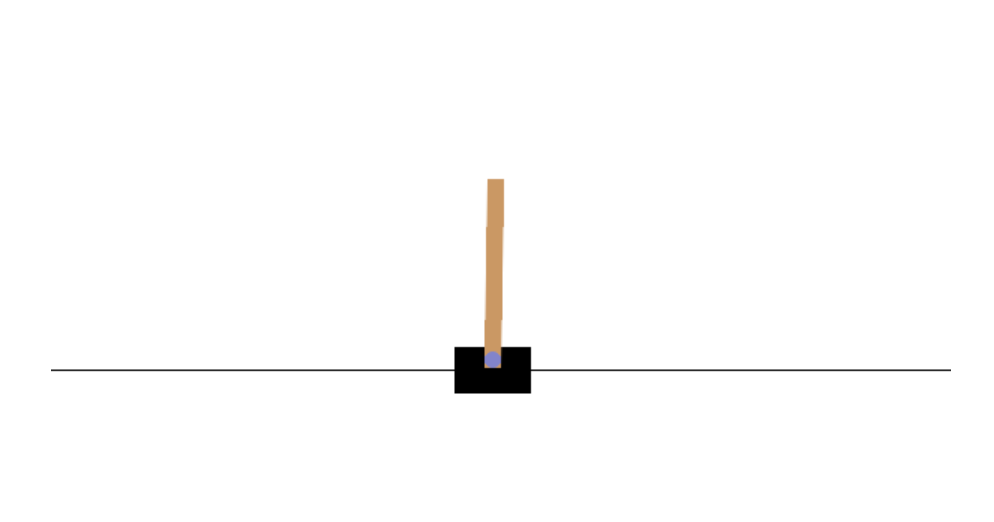
\includegraphics[width=0.5\linewidth]{img/cartpole.png}
    \caption{The OpenAI Gym CartPole environment \citep{brockman2016openai} is a classic RL control task where the goal is to balance a pole on a cart by applying forces to move the cart left or right. The state consists of the cart's position and velocity and the pole's angle and angular velocity. The episode ends if the cart moves out of bounds or the pole falls beyond a threshold angle.}
    \label{fig: cartpole intro}
\end{figure}

\begin{algorithm}[htbp]
    \caption{CartPole MRP and Feature Generation} \label{alg:cartpole generation}
    \begin{algorithmic}[1]
    \STATE \textbf{Input:} feature dimension $d$, action space $\fA = \qty{0,1}$, joint distribution over CartPole parameters $\Delta_\Psi$, joint distribution over features and rewards $\Delta_{\phi,r}$
    \STATE $\Psi \sim \Delta_\Psi$ \CommentSty{\, // sample CartPole parameter}
    \STATE $p_0 \gets \uniform{(-0.05, 0.05)^4}$ \CommentSty{\, // CartPole initial distribution}
    \STATE $\phi, \, r \gets \Delta_{\phi,r}(d)$ \CommentSty{\, // sample features and rewards}
    \STATE $\epsilon \sim \uniform{(0,1)}$ \CommentSty{\, // sample random policy parameter}
        % \FOR {$s \in \fS$}
        % \STATE $b \gets \beta(s,m)$  \CommentSty{\, // bin the state}
        % \STATE $\pi_\epsilon(\cdot|s) \gets \text{Bernoulli}(\epsilon)$ \CommentSty{\, // random policy}
            % \FOR{$s' \in \fS$}
                 \STATE $p(s'|s) \gets \sum_{a \in \fA}\pi_{\epsilon}(a|s) p_{\text{CartPole}}(s'|s,a ; \Psi)$ \CommentSty{\, // CartPole state transition}
            % \ENDFOR
    % \ENDFOR
    \STATE \textbf{Output:} MRP $(p_0, p, r)$ and feature map $\phi$
    \end{algorithmic}
\end{algorithm}

\subsection{Experimental Results of Pre-training with CartPole}
In our experiments in Figure \ref{fig: cartpole l=3}, we pre-train a 3-layer autoregressive transformer using Algorithm \ref{deep td}, where the task distribution $d_{\text{task}}$ is generated using CartPole MRPs (see Algorithm \ref{alg:cartpole generation}) with a feature vector of dimension $d = 4$. We used a significantly larger context window length $n=250$. Despite the increased complexity of the transition dynamics in the CartPole environment compared to Boyan's chain environment used in Figure \ref{fig: linear parameter convergence auto l=3}, our results demonstrate that $P_0$ and $Q_0$ still converge to the construction in Theorem \ref{thm: TD(0)} (up to some noise), which we proved exactly implements TD(0). 

It is worth noting that our theoretical results (Theorem \ref{thm: fixed point analysis}), which prove that the weights implementing TD are in the invariant set of the updates in Algorithm \ref{deep td}, do not depend on any specific properties of the environment $p$. Thus, it is unsurprising that TD(0) emerges naturally even after pre-training on environments with complicated dynamics.


\begin{figure}[th!]
\centering
  \begin{subfigure}[b]{0.39\textwidth}
    \centering
    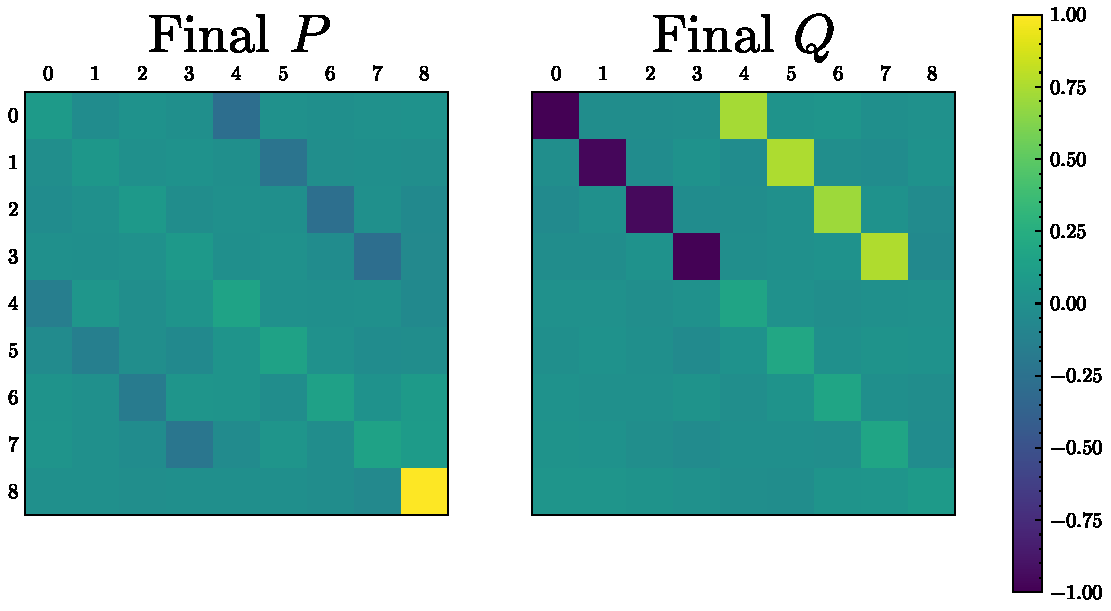
\includegraphics[width=\textwidth]{img/cartpole/PQ_mean_0_10000.pdf}
    \caption{Learned $P_0$ and $Q_0$ after 10000 MRPs}
    \label{fig: cartpole parameters}
  \end{subfigure}
  \begin{subfigure}[b]{0.6\textwidth}
    \centering
    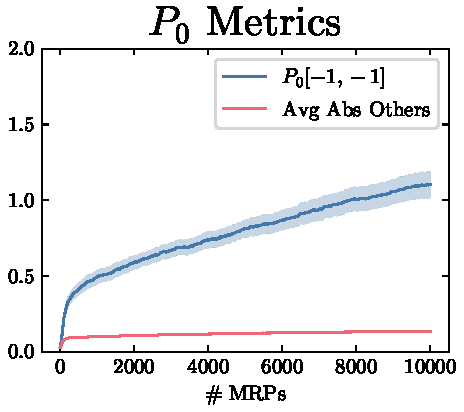
\includegraphics[width=0.4\textwidth]{img/cartpole/P_metrics_0.pdf}
    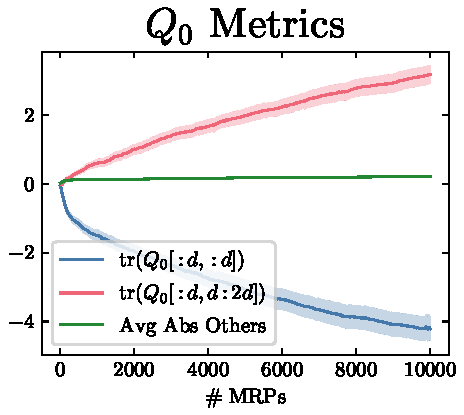
\includegraphics[width=0.4\textwidth]{img/cartpole/Q_metrics_0.pdf}
    \caption{Element-wise learning progress of $P_0$ and $Q_0$}
    \label{fig: cartpole metrics}
  \end{subfigure}
 \caption{Visualization of the learned transformers and the learning progress after pretraining with the CartPole environment for 10,000 MRPs.
 Both (a) and (b) are averaged across 30 seeds and the shaded regions in (b) denote the standard errors.}
  \label{fig: cartpole l=3} 
\end{figure}


\section{Investigation of In-Context TD with RNN}
We have focused primarily on the transformer's capability to implement TD in context.
Before transformers, the canonical architecture to tackle sequence modelling problems is the recurrent neural network (RNN)~\citep{ elman1990finding, bengio2017deep}.
Thus, it's worth investigating the algorithmic capacity of RNN in implementing TD in its forward pass.
In particular, we try to answer the following two questions in this section:
\begin{enumerate}
    \item Can RNN implement TD in context? \label{question: rnn can}
    \item Does in-context TD emerge in RNN via multi-task pre-training? \label{question: rnn do}
\end{enumerate}

A canonical deep RNN with $L$ layers is parameterized by $\qty{W_{ax}^{(l)}, W_{aa}^{(l)}, b^{(l)}_{a}}_{l=0,\dots,L-1}$.
Let $m$ denote the dimension of the raw input tokens and $h$ denote that of the hidden states, respectively.
Then, we have $W_{ax}^{(0)} \in \R^{h\times m}$, $W_{ax}^{(l)} \in \R^{h\times h}$ for $l= 1, \dots, L-1$, and $ W_{aa}^{(l)} \in \R^{h\times h}$, $ b^{(l)}_a \in \R^h$ for $l=0,\dots,L-1$.
Let $x_t^{(l)}$ denote the input token and $a_t^{(l)}$ denote the hidden state for layer $l$ at time step $t$.
Unlike transformers that process the whole sequence at once, an RNN processes one token after another sequentially by updating the hidden states.
The hidden state evolves according to
\begin{align}
    a_{t+1}^{(l)} = f\qty(W_{ax}^{(l)}x_t^{(l)} + W_{aa}^{(l)}a_t^{(l)} + b_a^{(l)})
\end{align}
where $f$ is an activation function.
In addition, we have $x_t^{(l)} = a_t^{(l-1)}$ for all $t$ and $l = 1,\dots, L-1$.
In other words, the input to the next depth is the hidden state from the previous depth except for the first layer.
The initial hidden states $a_0^{(l)}, l = 0, \dots, L-1$ are selected arbitrarily.
Popular options include zero initialization and random normal initialization.

When we apply RNN to policy evaluation, we are interested in predicting a scalar value at the end, also known as many-to-one prediction.
Suppose the input sequence has $n$ tokens one typically passes $a_n^{L-1}$, the final hidden state at the last recurrent layer, through a fully connected output layer $W_o \in \R^{1 \times h}$, such that
\begin{align}
    \hat{v} = W_o a_n^{L-1}.
\end{align}

\subsection{Theoretical Analysis of Linear RNN}
We first investigate Question~\ref{question: rnn can} via a theoretical analysis of RNN in the context of TD.
Due to the intractable difficulty of nonlinear activations present in deep neural network analysis, we resort to analyzing a single-layer linear RNN, i.e., $L=1$ and $f$ is the identity mapping.
Hence, we will drop the superscript indicating the layer index and $f$ in our notation to simplify the presentation.
We shall also remove the bias term $b_{a}$ because it is a constant independent of the context.
Under this formulation, the hidden state evolves according to
\begin{align}
    a_{t+1} = W_{ax} x_t + W_{aa} a_t.
\end{align}
If we initialize $a_0 = 0$, we then have
\begin{align}
    a_0 &= 0\\
    a_1 &= W_{aa} a_0 + W_{ax} x_0 = W_{ax} x_0\\
    a_2 &= W_{aa} a_1 + W_{ax} x_1 = W_{ax} x_1 + W_{aa}W_{ax} x_0\\
    a_3 &= W_{aa} a_2 + W_{ax} x_2 = W_{ax} x_2 + W_{aa}W_{ax} x_1 + W_{aa}^2W_{ax} x_0\\
    &\vdots
\end{align}
Assuming a sequence of $n$ tokens, the final hidden state $a_n$ is 
\begin{align}
    a_n = \sum_{t=0}^{n-1} W_{aa}^{n-t-1} W_{ax} x_t.
\end{align}
Applying a linear output layer $W_o \in \R^{1 \times h}$ to the hidden state for value prediction, we then get
\begin{align}
\label{eq: linear rnn prediction}
    \hat{v} = W_o a_n = \sum_{t=0}^{n-1} W_o W_{aa}^{n-t-1} W_{ax} x_t 
    = \sum_{t=0}^{n-1} w_t^\top x_t,
\end{align}
where $w_t \doteq \qty(W_o W_{aa}^{n-t-1} W_{ax})^\top \in \R^h$ is a vector.
\eqref{eq: linear rnn prediction} demonstrates that the predicted value is the sum of the inner product between each token and some vector for linear RNN.
Recall that each context token $x_t$ for in-context TD is defined as
\begin{align}
    x_t \doteq \mqty[\phi_t\\\gamma\phi'_t\\R_t],
\end{align}
corresponding to column $t$ of the prompt $Z$.
Hence, we can write
\begin{align}
    \hat{v} = \sum_{t=0}^{n-1} w_t^\top \mqty[\phi_t\\\gamma\phi'_t\\R_t].
\end{align}
Under this representation, it is impossible to construct the TD error, not to mention applying the semi-gradient term.
Therefore, it is safe for us to claim that linear RNN is incapable of implementing TD in its forward pass.
This result is easily extendable to the multi-layer case since it is only performing linear combinations of the tokens, thus reducible to the format of \eqref{eq: linear rnn prediction}.
One important insight gained by comparing the forward pass of an RNN and a transformer under linear activation is that one at least needs $x_t^\top Q x_t$ where $Q$ is a square matrix to have any hope to compute the TD error, which is necessary for TD.
Therefore, we speculate that a deep RNN equipped with a common nonlinear activation such as $\tanh$ and $\text{ReLU}$ is also unable to implement TD in context.
We will leave the investigation to Question~\ref{question: rnn do}.
For now, we can confidently give a negative answer to Question~\ref{question: rnn can} concerning linear RNNs.

\subsection{Multi-task TD with Deep RNN}
We answer Question~\ref{question: rnn do} via an empirical study with a deep RNN.
We employ a 3-layer RNN with a hidden state dimension of $h=4$ and $\tanh$ as the activation function and train it via multi-task TD (Algorithm~\ref{deep td}) on 4,000 randomly generated Boyan's chain MRPs with a feature dimension of $d=4$.
Since we cannot apply a mask $M$ like in the transformer to distinguish the query from the context, we instead append a binary flag to each token for the same purpose.
Suppose there are $n$ context columns, the prompt $Z$ has the form
\begin{align}
    Z = \mqty[\phi_1 & \phi_2 & \dots & \phi_n & \phi_{n+1}\\
              \gamma\phi'_1 & \gamma\phi'_2 & \dots &\gamma\phi'_n & 0\\
              R_1 & R_2 & \dots & R_n & 0\\
              0 & 0 & \dots & 0 & 1
              ] \in \R^{(2d + 2) \times (n+1)}.
\end{align}
The forward pass of the deep RNN processes the tokens sequentially in the prompt to update the hidden states.
The final hidden state of the last layer of the RNN is fed into a fully connected layer to output a scalar value prediction.
Figure~\ref{fig: rnn msve vs mrp} shows the learning curve of the RNN throughout the multi-task TD training.
The MSVE decreases for the first 1,000 MRPs and stays low for the remainder of the training.
Thus, some learning occurs during the training of RNN.
However, it is unclear whether it is implementing in-context TD.
To clarify, we use the last checkpoint of the model and repeat the same experiment used to generate Figure~\ref{fig: icrl demo}.
We gradually increase the context length and verify if the MSVE drops as observed in the transformers.
We run the experiment on the Loop environment used to generate Figure~\ref{fig: icrl demo} and the Boyan's chain environment used for training for 500 instances each to produce Figure~\ref{fig: msve vs context length rnn}.
The MSVE increases with context length in both environments for the trained RNN, exhibiting a trend opposite to the transformer.
Furthermore, the standard errors are much higher than in Figure~\ref{fig: icrl demo} despite having more runs.
Therefore, the prediction does not improve with more context data for the RNN, indicating the absence of any in-context policy evaluation algorithms.
Consequently, the answer to Question~\ref{question: rnn do} is again negative.
\begin{figure}[htbp]
    \centering
    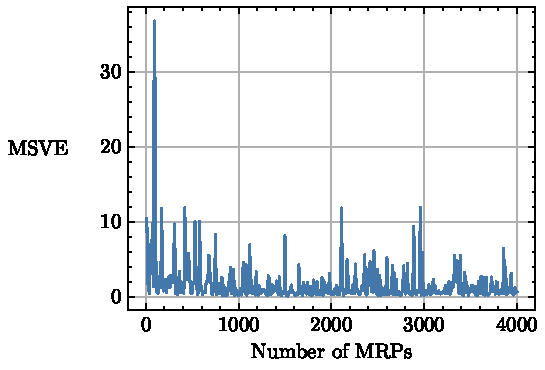
\includegraphics[width=0.6\textwidth]{img/rnn/msve_vs_mrp.pdf}
    \caption{RNN MSVE against the number of MRPs in multi-task TD training.}
    \label{fig: rnn msve vs mrp}
\end{figure}

\begin{figure}[htbp]
\centering
    \begin{subfigure}[b]{0.45\textwidth}
        \centering
        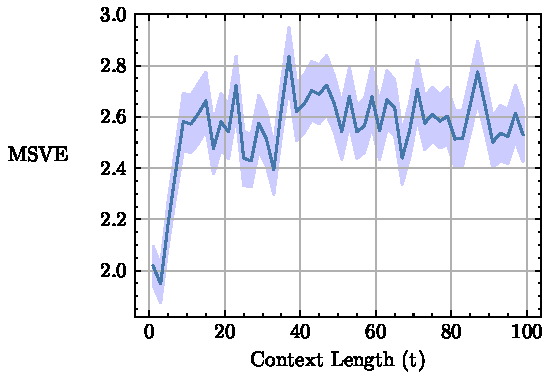
\includegraphics[width=\textwidth]{img/rnn/msve_vs_context_length_loop.pdf}
        \caption{Loop}
    \end{subfigure}
    \begin{subfigure}[b]{0.45\textwidth}
        \centering
        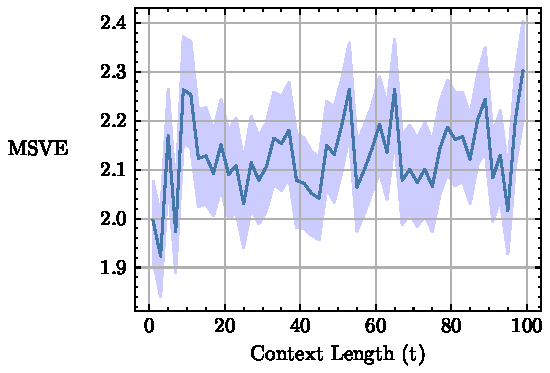
\includegraphics[width=\textwidth]{img/rnn/msve_vs_context_length_boyan.pdf}
        \caption{Boyan's chain}
    \end{subfigure}
    \caption{MSVE vs. context length with the trained RNN. The shaded regions are the standard errors.}
  \label{fig: msve vs context length rnn} 
\end{figure}


\section{Numerical Verification of Proofs} \label{appendix: numerical verification}
We provide numerical verification for our proofs by construction (Theorem~\ref{thm: TD(0)}, Corollary~\ref{corollary: true RG}, Corollary~\ref{thm: TD(0) lambda}, and Theorem~\ref{thm two head average reward TD}) as a sanity check.
In particular,
we plot $\log \abs{-\indot{\phi_n}{w_l} - y_l^{n+1}}$ against the number of layers $l$.
For example, for Theorem~\ref{thm: TD(0)},
we first randomly generate $Z_0$ and $\qty{C_l}$.
Then $y_l^{(n+1)}$ is computed by unrolling the transformer layer by layer following~\eqref{eq: Z_l update} while $w_l$ is computed iteration by iteration following~\eqref{eq: TD(0) w_update}.
We use double-precision floats and run for 30 seeds, each with a new prompt.
As shown in Figure~\ref{fig: theory verification},
even after 40 layers/iterations, 
the difference is still in the order of $10^{-10}$.
It is not strictly 0 because of numerical errors.
It sometimes increases because of the accumulation of numerical errors.

% We numerically verify our theory by comparing the linear transformers we've proven to implement batch TD(0), residual gradient, TD($\lambda$) and average reward TD against the explicit implementations.
% For all the experiments, we use a feature dimension of 3, a context length of 100 and 40 layers.
% We arbitrarily choose $\lambda = 0.5$ for TD($\lambda$).
% Recall that one layer corresponds to one step of weight update using the context.
% At each layer $l$, we record the absolute difference in their value predictions
% \begin{align}
    % \abs{v_l^\tf - v_l^*},
% \end{align}
% where we denote $v_l^\tf$ as the prediction made by the linear transformer and $v_l^*$ as the value learned by the corresponding explicit algorithm given the same prompt.
% We use a double-precision floating point and run for 30 seeds, each with a new prompt, and get Figure~\ref{fig: theory verification}.
% We see that TD(0) remains numerically stable throughout the unrolling of the model and algorithm.
% The other three models accumulate numerical errors steadily as we unroll them.
% The linear transformers of TD($\lambda$) and average reward TD accumulate errors at approximately the same rate, while the model of residual gradient gains numerical errors at approximately half of their rate in the log scale.
% As the prediction errors are negligible even after 40 steps of unrolling and the standard errors are virtually invisible, we are confident in the correctness of our theorems.
\begin{figure}[ht!]
    \centering
    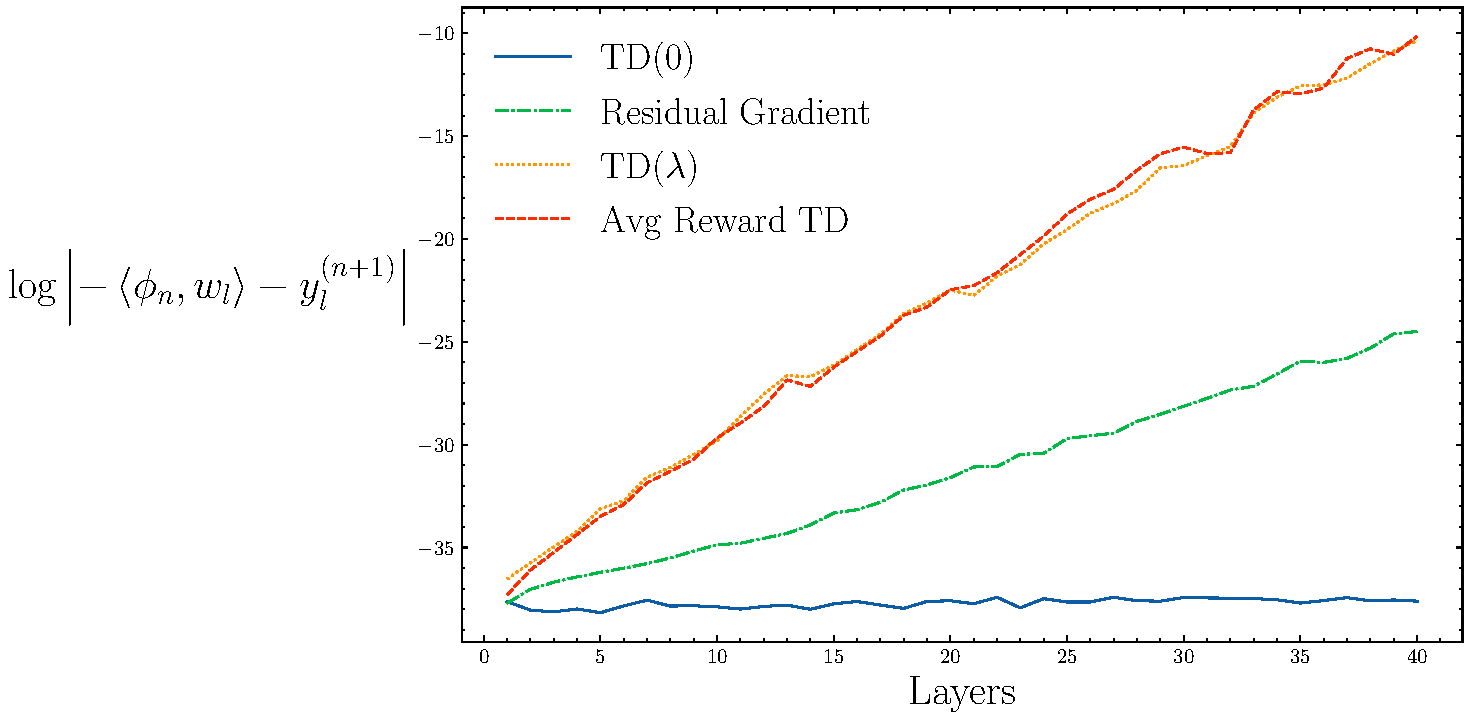
\includegraphics[width=0.6\textwidth]{img/theory_verification.pdf}
    \caption{Differences between transformer output and batch TD output.
    Curves are averaged over 30 random seeds with the (invisible) shaded region showing the standard errors. 
    }
    \label{fig: theory verification}
\end{figure}
\clearpage

%%%%%%%%%%%%%%%%%%%%%%%%%%%%%%
%END DOCUMENT
%%%%%%%%%%%%%%%%%%%%%%%%%%%%%%
\end{document}